%%%%%%%%%%%%%%%%%%%%%%%%%%%%%%%%%%%%%%%%%
% Masters/Doctoral Thesis 
% LaTeX Template
% Version 2.5 (27/8/17)
%
% This template was downloaded from:
% http://www.LaTeXTemplates.com
%
% Version 2.x major modifications by:
% Vel (vel@latextemplates.com)
%
% This template is based on a template by:
% Steve Gunn (http://users.ecs.soton.ac.uk/srg/softwaretools/document/templates/)
% Sunil Patel (http://www.sunilpatel.co.uk/thesis-template/)
%
% Template license:
% CC BY-NC-SA 3.0 (http://creativecommons.org/licenses/by-nc-sa/3.0/)
%
%%%%%%%%%%%%%%%%%%%%%%%%%%%%%%%%%%%%%%%%%

%----------------------------------------------------------------------------------------
%	PACKAGES AND OTHER DOCUMENT CONFIGURATIONS
%----------------------------------------------------------------------------------------

%%----------------------------------------------------------------------------------------
%	PACKAGES AND OTHER DOCUMENT CONFIGURATIONS
%----------------------------------------------------------------------------------------

\documentclass[
11pt, % The default document font size, options: 10pt, 11pt, 12pt
%oneside, % Two side (alternating margins) for binding by default, uncomment to switch to one side
english, % ngerman for German
singlespacing, % Single line spacing, alternatives: onehalfspacing or doublespacing
%draft, % Uncomment to enable draft mode (no pictures, no links, overfull hboxes indicated)
%nolistspacing, % If the document is onehalfspacing or doublespacing, uncomment this to set spacing in lists to single
%liststotoc, % Uncomment to add the list of figures/tables/etc to the table of contents
%toctotoc, % Uncomment to add the main table of contents to the table of contents
%parskip, % Uncomment to add space between paragraphs
%nohyperref, % Uncomment to not load the hyperref package
headsepline, % Uncomment to get a line under the header
%chapterinoneline, % Uncomment to place the chapter title next to the number on one line
%consistentlayout, % Uncomment to change the layout of the declaration, abstract and acknowledgements pages to match the default layout
]{MastersDoctoralThesis} % The class file specifying the document structure

\usepackage[utf8]{inputenc} % Required for inputting international characters
\usepackage[T1]{fontenc} % Output font encoding for international characters

\usepackage{mathpazo} % Use the Palatino font by default


\usepackage[
backend=biber,
style=alphabetic,
sorting=ynt
]{biblatex}

\addbibresource{sample.bib} % The filename of the bibliography

\usepackage[autostyle=true]{csquotes} % Required to generate language-dependent quotes in the bibliography
%----------------------------------------------------------------------------------------
%	PACKAGES AND OTHER DOCUMENT CONFIGURATIONS
%----------------------------------------------------------------------------------------

\documentclass[
draft, % To disable image rendering
11pt, % The default document font size, options: 10pt, 11pt, 12pt
oneside, % Two side (alternating margins) for binding by default, uncomment to switch to one side
english, % Language
singlespacing, % Single line spacing, alternatives: onehalfspacing or doublespacing
%draft, % Uncomment to enable draft mode (no pictures, no links, overfull hboxes indicated)
%nolistspacing, % If the document is onehalfspacing or doublespacing, uncomment this to set spacing in lists to single
%liststotoc, % Uncomment to add the list of figures/tables/etc to the table of contents
%toctotoc, % Uncomment to add the main table of contents to the table of contents
parskip, % Uncomment to add space between paragraphs
%nohyperref, % Uncomment to not load the hyperref package
headsepline, % Uncomment to get a line under the header
%chapterinoneline, % Uncomment to place the chapter title next to the number on one line
%consistentlayout, % Uncomment to change the layout of the declaration, abstract and acknowledgements pages to match the default layout
]{MastersDoctoralThesis} % The class file specifying the document structure

\usepackage{svg}
\usepackage{listings}
\usepackage{xcolor}
\usepackage{float}
\usepackage{caption}
\usepackage{subcaption}
\usepackage{datetime}
\usepackage[final]{hyperref}
%\usepackage{comment}

\newdateformat{monthyeardate}{\monthname[\THEMONTH] \THEYEAR}

\definecolor{codegreen}{rgb}{0,0.6,0}
\definecolor{codegray}{rgb}{0.5,0.5,0.5}
\definecolor{codepurple}{rgb}{0.58,0,0.82}
\definecolor{backcolour}{rgb}{0.95,0.95,0.92}

\lstdefinestyle{mystyle}{
    backgroundcolor=\color{backcolour},   
    commentstyle=\color{codegreen},
    keywordstyle=\color{magenta},
    numberstyle=\tiny\color{codegray},
    stringstyle=\color{codepurple},
    basicstyle=\ttfamily\footnotesize,
    breakatwhitespace=faòse,         
    breaklines=true,                 
    captionpos=b,                    
    keepspaces=true,                 
    numbers=left,                    
    numbersep=5pt,                  
    showspaces=false,                
    showstringspaces=false,
    showtabs=false,                  
    tabsize=2
}

\lstset{style=mystyle}

\usepackage[utf8]{inputenc} % Required for inputting international characters
\usepackage[T1]{fontenc} % Output font encoding for international characters

\usepackage{mathpazo} % Use the Palatino font by default
\usepackage{amsmath}
\usepackage{bbm}

\usepackage[
backend=biber,
style=numeric,
sorting=nty
]{biblatex}

\addbibresource{sample.bib} % The filename of the bibliography

\usepackage[autostyle=true]{csquotes} % Required to generate language-dependent quotes in the bibliography

%----------------------------------------------------------------------------------------
%	MARGIN SETTINGS
%----------------------------------------------------------------------------------------

\geometry{
	paper=a4paper, % Change to letterpaper for US letter
	inner=2.5cm, % Inner margin
	outer=3.8cm, % Outer margin
	bindingoffset=.5cm, % Binding offset
	top=1.5cm, % Top margin
	bottom=1.5cm, % Bottom margin
	%showframe, % Uncomment to show how the type block is set on the page
}

%----------------------------------------------------------------------------------------
%	THESIS INFORMATION
%----------------------------------------------------------------------------------------

%----------------------------------------------------------------------------------------
%	THESIS INFORMATION
%----------------------------------------------------------------------------------------

\author{Morgan \textsc{Casale}} % Your name, this is used in the title page and abstract, print it elsewhere with \authorname

\subject{Mechatronic Engineering} % Your subject area, this is not currently used anywhere in the template, print it elsewhere with \subjectname
\keywords{} % Keywords for your thesis, this is not currently used anywhere in the template, print it elsewhere with \keywordnames

\university{\href{https://www.polito.it/}{Politecnico di Torino}} % Your university's name and URL, this is used in the title page and abstract, print it elsewhere with \univname
\otheruniversity{\href{https://www.unisi.it/}{Università di Siena}}

\department{\href{https://www.dauin.polito.it} {Department or Control and Computer Engineering}} % Your department's name and URL, this is used in the title page and abstract, print it elsewhere with \deptname
\supervisordepartment{\href{https://www.det.polito.it/} {DET}}
\otherdepartment{\href{https://www.diism.unisi.it} {DIISM}}

\group{\href{https://sirslab.dii.unisi.it/}{SIRSLab}} % Your research group's name and URL, this is used in the title page, print it elsewhere with \groupname

\faculty{Mechatronic Engineering} % Your faculty's name and URL, this is used in the title page and abstract, print it elsewhere with \facname


\thesistitle {Study of flexible PCB coils in haptic applications} % Your thesis title, this is used in the title and abstract, print it elsewhere with \ttitle
\supervisor {Alessandro \textsc{Rizzo} \\(\textit{\univname \:- \supdeptname})} % Your supervisor's name, this is used in the title page, print it elsewhere with \supname
\cosupervisor{Domenico \textsc{Prattichizzo} \\(\textit{\otherunivname \:- \otherdeptname \:- \groupname})} % Your co-supervisor's name, this is used in the title page, print it elsewhere with \cosupname
\cocosupervisor{Leonardo \textsc{Franco} \\(\textit{\otherunivname \:- \otherdeptname \:- \groupname})} % Your co-supervisor's name, this is used in the title page, print it elsewhere with \cosupname
\examiner{} % Your examiner's name, this is not currently used anywhere in the template, print it elsewhere with \examname
\degree{} % Your degree name, this is used in the title page and abstract, print it elsewhere with \degreename
\addresses{} % Your address, this is not currently used anywhere in the template, print it elsewhere with \addressname


\AtBeginDocument{
    \hypersetup{pdftitle=\ttitle} % Set the PDF's title to your title
    \hypersetup{pdfauthor=\authorname} % Set the PDF's author to your name
    \hypersetup{pdfkeywords=\keywordnames} % Set the PDF's keywords to your keywords
}

%----------------------------------------------------------------------------------------
%	BEGIN DOCUMENT
%----------------------------------------------------------------------------------------

\begin{document}

\frontmatter % Use roman page numbering style (i, ii, iii, iv...) for the pre-content pages

\pagestyle{plain} % Default to the plain heading style until the thesis style is called for the body content

%----------------------------------------------------------------------------------------
%	TITLE PAGE
%----------------------------------------------------------------------------------------

%----------------------------------------------------------------------------------------
%	TITLE PAGE
%----------------------------------------------------------------------------------------

\begin{titlepage}
\begin{center}

%\vspace*{.06\textheight}
{\scshape\LARGE \univname\par}\vspace{1.5cm} % University name
\textsc{\Large Master Degree Thesis}\\[0.5cm] % Thesis type
\Large\deptname\\[0.5cm] %department name
\Large\facname\\[0.5cm] %faculty name
\textit{\normalsize a.y. 2023/2024} %academic year

\vfill
\includesvg[width = 1\textwidth]{Figures/Title/Logo_Polito.svg} % University/department logo - uncomment to place it
\vfill

%\HRule \\[0.4cm] % Horizontal line
{\huge \bfseries \ttitle\par}\vspace{0.4cm} % Thesis title
%\HRule \\[1.5cm] % Horizontal line
 

%\large \textit{A thesis submitted in fulfillment of the requirements\\ for the degree of \degreename}\\[0.3cm] % University requirement text
%\textit{in the}\\[0.4cm]
%\groupname\\

\vfill

\begin{minipage}[t]{0.4\textwidth}
\begin{flushleft} \large
\emph{Supervisors:} \\[0.2cm]
\supname\\[0.3cm] % Supervisor name
\cosupname\\[0.3cm] %Co-supervisor name
\cocosupname
\end{flushleft}
\end{minipage}
\begin{minipage}[t]{0.4\textwidth}
\begin{flushright} \large
\emph{Candidate:}\\[0.2cm]
\authorname % Author name
\end{flushright}
\end{minipage}\\[1cm]

{\large \monthyeardate\today}\\[4cm] % Date
 
\end{center}
\end{titlepage}

%----------------------------------------------------------------------------------------
%	DECLARATION PAGE
%----------------------------------------------------------------------------------------

%%----------------------------------------------------------------------------------------
%	DECLARATION PAGE
%----------------------------------------------------------------------------------------

\begin{declaration}
\addchaptertocentry{\authorshipname} % Add the declaration to the table of contents
\noindent I, \authorname, declare that this thesis titled, \enquote{\ttitle} and the work presented in it are my own. I confirm that:

\begin{itemize} 
\item This work was done wholly or mainly while in candidature for a research degree at this University.
\item Where any part of this thesis has previously been submitted for a degree or any other qualification at this University or any other institution, this has been clearly stated.
\item Where I have consulted the published work of others, this is always clearly attributed.
\item Where I have quoted from the work of others, the source is always given. With the exception of such quotations, this thesis is entirely my own work.
\item I have acknowledged all main sources of help.
\item Where the thesis is based on work done by myself jointly with others, I have made clear exactly what was done by others and what I have contributed myself.\\
\end{itemize}
 
\noindent Signed:\\
\rule[0.5em]{25em}{0.5pt} % This prints a line for the signature
 
\noindent Date:\\
\rule[0.5em]{25em}{0.5pt} % This prints a line to write the date
\end{declaration}

\cleardoublepage

%----------------------------------------------------------------------------------------
%	QUOTATION PAGE
%----------------------------------------------------------------------------------------

%%----------------------------------------------------------------------------------------
%	QUOTATION PAGE
%----------------------------------------------------------------------------------------

\vspace*{0.2\textheight}

\noindent\enquote{\itshape Thanks to my solid academic training, today I can write hundreds of words on virtually any topic without possessing a shred of information, which is how I got a good job in journalism.}\bigbreak

\hfill Dave Barry

%----------------------------------------------------------------------------------------
%	ABSTRACT PAGE
%----------------------------------------------------------------------------------------

%----------------------------------------------------------------------------------------
%	ABSTRACT PAGE
%----------------------------------------------------------------------------------------

\begin{abstract}
\addchaptertocentry{\abstractname} % Add the abstract to the table of contents
The world of haptic is an emerging field of research with rapidly evolving technologies.
Researchers are still looking for the optimal solution to create a haptic device that can provide a
realistic touch sensation. Vibrations, forces, and temperatures are the stimuli involved in the
majority of the touch experience.
For what concerns the rendering of texture, i.e., generating vibratory cues, the most widespread technology is high-performance piezo actuators, but even if this technology has multiple limitations.
The most critical ones are their limited capability of generating low-frequency responses
and their lack of flexible models.
These characteristics are crucial for the creation of a realistic haptic interface that could also be
easily integrated into wearable devices.

This thesis aims at investigating the use of flexible PCB coils in haptic applications.
Flexible PCB coils are a new technology which can be used to create voice actuator-style haptic
interfaces that can withstand bending stresses and produce low-frequency vibrations.
Voice-coil actuators are systems based on the electromagnetic force interaction between a coil
and a magnet.
This force can be harnessed with the use of a membrane to transfer vibrations to human skin.

The first part of the thesis focuses on the physics of such a device with the creation of a
mathematical model of the entire force transmission chain, considering also how finger-pulp skin
reacts to the device stimuli at different frequencies and amplitudes.

Next, the electronics required to drive the proposed device is
presented.

Finally, the last part reports the design and testing of a series of prototypes
that will help us understand the limitations and potential of this technology.

\end{abstract}

%----------------------------------------------------------------------------------------
%	LIST OF CONTENTS/FIGURES/TABLES PAGES
%----------------------------------------------------------------------------------------

%----------------------------------------------------------------------------------------
%	LIST OF CONTENTS/FIGURES/TABLES PAGES
%----------------------------------------------------------------------------------------

\tableofcontents % Prints the main table of contents

\listoffigures % Prints the list of figures

{\let\cleardoublepage\relax \listoftables } % Prints the list of tables

%----------------------------------------------------------------------------------------
%	ABBREVIATIONS
%----------------------------------------------------------------------------------------
\begin{abbreviations}{ll} % Include a list of abbreviations (a table of two columns)
    \textbf{RMS} & \textbf{R}oot \textbf{M}ean \textbf{S}quare\\
    \textbf{PCB} & \textbf{P}rinted \textbf{C}ircuit \textbf{B}oard\\
    \textbf{AC} & \textbf{A}lternated \textbf{C}urrent\\
    \textbf{DC} & \textbf{D}irect \textbf{C}urrent\\
    \textbf{re} & \textbf{re}ferring to\\
    \textbf{PLA} & \textbf{P}oly\textbf{L}actic \textbf{A}cid\\
    \textbf{ABS} & \textbf{A}crylonitrile \textbf{B}utadiene \textbf{S}tyrene\\
    \textbf{TPU} & \textbf{T}hermo\textbf{P}lastic \textbf{U}rethane\\
    \textbf{BVOH} & \textbf{B}utylene \textbf{V}inyl \textbf{O}l\textbf{H}exanoate\\
    \textbf{FEM} & \textbf{F}inite \textbf{E}lement \textbf{M}ethod\\
\end{abbreviations}


%----------------------------------------------------------------------------------------
%	SYMBOLS
%----------------------------------------------------------------------------------------
{\let\cleardoublepage\relax
    \begin{symbols}{lll} % Include a list of Symbols (a three column table)
        % Symbol & Name & Unit \\
        % \midrule
        % $E_{CNN}$ & Landmark Regression error & px \\
        % $E_{NN}$ & Landmark Mapping error & cm\\
        % $E_{T}$ & Translation error & cm \\
        % $E_{R}$ & Rotation error & ° \\
        % $S_{T}$ & Translation score & - \\
        % $S_{R}$ & Rotation error & rad \\
        \textbf{m} & \textbf{m}eter & Distance\\
        \textbf{s} & \textbf{s}econd & Time\\
        \textbf{Hz} & \textbf{H}ertz & Frequency\\
        
        \textbf{dB} & \textbf{D}ecibel & Intensity\\

        \textbf{g} & \textbf{g}ram & Mass\\
        \textbf{N} & \textbf{N}ewton & Force\\
        \textbf{Pa} & \textbf{P}ascal & Pressure\\

        \textbf{V} & \textbf{V}olt & Electrical Voltage\\
        \textbf{A} & \textbf{A}mpere & Electrical Current\\
        \textbf{W} & \textbf{W}att & Electrical Power\\
        \textbf{$\Omega$} & Ohm & Electrical Resistance\\  
        \textbf{F} & \textbf{F}arad & Electrical Capacitance\\
        \textbf{H} & \textbf{H}enry & Electrical Inductance\\

        \textbf{T} & \textbf{T}esla & Magnetic Flux Density\\
        \textbf{Wb} & \textbf{W}e\textbf{b}er & Magnetic Flux\\ 
    \end{symbols}
}

%----------------------------------------------------------------------------------------
%	DEDICATION
%----------------------------------------------------------------------------------------

%\dedicatory{For/Dedicated to/To my\ldots} 

%----------------------------------------------------------------------------------------
%	THESIS CONTENT - CHAPTERS
%----------------------------------------------------------------------------------------

\mainmatter % Begin numeric (1,2,3...) page numbering

\pagestyle{thesis} % Return the page headers back to the "thesis" style

% Include the chapters of the thesis as separate files from the Chapters folder
% Uncomment the lines as you write the chapters

% Chapter Template
\chapter{Introduction} % Main chapter title

\label{Chapter1} % Change X to a consecutive number; for referencing this chapter elsewhere, use \ref{ChapterX}

%----------------------------------------------------------------------------------------
%	SECTION 1
%----------------------------------------------------------------------------------------
\section{Thesis objective}

The world of haptics is an exciting field in the world of robotics, it was born from the will to bridge even further the digital world with the real one.
After digitalizing the sense of sight and hearing, the sense of touch is the next logical frontier to conquer.
The sense of touch is a very important sense for humans, it is the first sense that develops in the womb and it is the first sense that is used by a newborn to explore the world.
It is also the sense that is the most difficult to replicate in a virtual environment.

In past years there has been a lot of research in the field of haptics, but the field is still in its infancy.
Even if the current best haptic devices are able to provide vibration, force and temperature cues to the user, they are still far from being able to replicate the sense of touch realistically.

The most important components of haptics are vibrations and forces, they are the most common cues that are used to convey information to the user.
The generation of these types of cues is usually handled by piezoelectric actuators as they can generate vibrations with a high bandwidth (especially in the high range) and precision exerting notable force.

The only drawbacks of piezoelectric actuators are that they are rigid components, they cannot be bent or stretched, and they are not able to generate forces in the low range.

The objective of this thesis is to study a different type of actuator, voice coils based on flexible coils, and to compare them with piezoelectric actuators.
The main advantage of voice coils is that they can generate vibration with enough force also at low frequencies. 
In this research, we want to understand if we can create a haptic device that can be stretchable and possibly wearable by using flexible coils.

We will study the strengths and weaknesses of such type of actuator and propose multiple designs for a haptic device created with this technology.

%----------------------------------------------------------------------------------------
%	SECTION 2
%----------------------------------------------------------------------------------------
\section{Necessary background (?)}
\label{Chapter1/Dataset}
The algorithm is designed around \textit{TASI EROSS IOD Simulated Dataset N°2}, which consists of grayscale images of the satellite; see figure \textbf{\ref{fig:Samples}}.\\
The training dataset is composed of sixteen trajectories each of 900 images. Each trajectory covers the distance range from 200 to 20 cm to the target and the difference between each subsequent frame captured by each camera is 0.2 cm. Each image is of size 512x512 pixels and it's paired with ground truth 6DOF poses (position and orientation).
\begin{figure}[th]
    \centering
    \includegraphics[scale=0.48]{Figures/Chapter1/DatasetExample.png}
    \caption[Sample images from \textit{TASI EROSS IOD Simulated Dataset N°2}]{Sample images from the \textit{TASI EROSS IOD Simulated Dataset N°2}}
    \label{fig:Samples}
\end{figure}
\newpage
The data acquisition has been performed as follow:
\begin{itemize}
    \item \textbf{Non Prepared scenario:} LAR view.
    \item \textbf{Natural Illumination:} Full illumination (sun @45°, 130k lux).
    \item \textbf{Illumination system:} ON (150lm x6 LEDs).
    \item \textbf{Simulated Camera Settings:}
        \begin{itemize}
            \item Shutter speed: 20
            \item ISO: 5
            \item Aperture: 4
            \item FOV: 67.8°
        \end{itemize}
    \item \textbf{Reference System:}
        \begin{itemize}
            \item Left-handed XYZ reference.
            \item Origin [0,0,0]:
            \begin{itemize}
                \item XY: zeroes on the vertical symmetry axis of the Target.
                \item Z: Positive towards contact, zeroed on the lowest contact point of the LAR.
            \end{itemize}
            \item All units are in centimeters (cm).
        \end{itemize}
    \item \textbf{Trajectories:}
        \begin{itemize}
            \item all trajectories follow the same XYZ coordinates.
            \item the rotation is considered with Euler angles as Pitch (around axis x), Yaw (around axis y) and Roll (around axis z), all positive counterclockwise. Trajectories' specifics are reported in table \textbf{\ref{tab:trajectories}}.
            \item Camera pointing XY in [-46, +20].
        \end{itemize}
\end{itemize}

\begin{figure}[th]
    \centering
    \includegraphics[scale=0.8]{Figures/Chapter1/UPS.png}
    \caption[Model's UPS]{Model's UPS}
    \label{fig:UPS}
\end{figure}

\begin{table}[H]
\caption{Specifics of the simulated training trajectories.}
\label{tab:trajectories}
\centering
\begin{tabular}{l | l l l}
\toprule
Trajectory & Roll(°) & Pitch(°) & Yaw(°)\\
\midrule
TRAY\_1 & 0 & 0 & 0\\
TRAY\_2 & 0 & 0 & -1\\
TRAY\_3 & 0 & 0 & -2\\
TRAY\_4 & 0 & 0 & -3\\
TRAY\_5 & 0 & 0 & -4\\
TRAY\_6 & 0 & 0 & -5\\
TRAY\_7 & 0 & 1 & 0\\
TRAY\_8 & 0 & 2 & 0\\
TRAY\_9 & 0 & 3 & 0\\
TRAY\_10 & 0 & 4 & 0\\
TRAY\_11 & 0 & 5 & 0\\
TRAY\_12 & -1 & 0 & 0\\
TRAY\_13 & -2 & 0 & 0\\
TRAY\_14 & -3 & 0 & 0\\
TRAY\_15 & -4 & 0 & 0\\
TRAY\_16 & -5 & 0 & 0\\
\bottomrule
\end{tabular}
\end{table}

The \textit{TASI EROSS IOD Simulated Dataset N°3} along with the \textit{Less\_Difficult\_Trajectory} and \textit{Difficult\_Trajectory} are used as the test dataset. The \textit{TASI EROSS N°3} is composed of two trajectories, each of which was captured with two different camera positions. Each trajectory has 900 images.\\
The \textit{TRAY\_A} starts with +15° on Yaw and linearly converge toward 0 on contact, while \textit{TRAY\_B}, \textit{Less\_Difficult\ Trajectory} and \textit{Difficult\_Trajectory} present multiple errors on RPY converging toward 0 on contact as well.


%----------------------------------------------------------------------------------------
%	SECTION 3
%----------------------------------------------------------------------------------------
\section{Thesis structure}
The thesis is structured in further five chapters:
\begin{description}
    \item[Chapter 2] - \textit{Background}:\\ This chapter provides a comprehensive overview of key concepts necessary for the correct understanding of this work, with a focus on monocular camera models, perspective projection, pose estimation, and a general introduction to deep learning models.
    \item[Chapter 3] - \textit{State-of-art}:\\ This chapter delves into monocular pose estimation methods, covering classic approaches like RANSAC and SfM, and exploring modern techniques such as end-to-end learning with networks like PoseNet and Mask R-CNN. The chapter also introduces feature learning, emphasizing CNN-based methods like HRNet for predicting 2D landmark locations. Moreover, some studies about spacecraft pose estimation and their use of deep learning architectures are presented. The chapter also delves into point set alignments, highlighting the widely used and advanced algorithms like Coherent Point Drift (CPD) technique employed in the method for final pose estimation.
    \item[Chapter 4] - \textit{Algorithms and Methods}: \\
    This chapter delves into the methodology's core algorithms and techniques. It outlines the offline architecture, detailing the 2D-3D correspondence process, landmark regression, and the neural network-based landmark mapping. The chapter then presents the online architecture, covering real-time processing and the Coherent Point Drift technique for pose estimation. Implementation challenges and dataset considerations are also discussed, providing a comprehensive overview of the applied methods.
    \item[Chapter 5] - \textit{Implementation and Experiments}:\\
    This chapter presents the tools and technologies employed for the project implementation and the evaluation metrics for pose estimation, Landmark Regression, Landmark Mapping are described. The chapter culminates in the assessment of both training and test datasets, showcasing the method's robustness and generalization across diverse scenarios. Overall, it provides comprehensive exploration of the research's implementation and experimentation phases.
    \item[Chapter 6] - \textit{Discussions and Conclusions}:\\
    The Chapter delves into challenges faced by on-board AI systems in space missions, focusing on verifiability and computational load. It emphasizes the significance of minimizing translation errors for accurate maneuvering in the proposed multi-model configuration. The section explores potential improvements, including enhanced landmark selection and strategies to fortify system robustness.
\end{description}

% Chapter Template

\chapter{Background} % Main chapter title

\label{Chapter2} % Change X to a consecutive number; for referencing this chapter elsewhere, use \ref{ChapterX}

%----------------------------------------------------------------------------------------
%	SECTION 1
%----------------------------------------------------------------------------------------
\section{Magnetic Coils}

% Subsection 1
\subsection{Brief History}

The connection between electricity and magnetism was first demonstrated by Hans Christian Oersted in 1820 when he observed that an electric current flowing through a wire could deflect a nearby magnetic needle.

Meanwhile, the creation of the first practical electromagnet is credited to William Sturgeon and André-Marie Ampère who after Oersted's discovery experimented with creating coil windings wrapped around an iron core which allowed them to achieve much stronger magnetic fields.

During the 1830's Michael Faraday's discovery of electromagnetic induction further advanced the understanding of magnetic fields and coils. Faraday demonstrated that a changing magnetic field could induce an electric current in a nearby conductor, laying the groundwork for transformers and modern electrical generators.

The latter half of the 19th century saw rapid advancements in electrical engineering. Innovations like early electric generators (dynamos), transformers, and electric motors heavily relied on magnetic coils for their operation. Researchers such as Nikola Tesla and Thomas Edison further developed these technologies.

Magnetic coils continue to play a vital role in various fields, including power generation, telecommunications, electronics, and medical imaging (such as MRI machines). With advancements in materials science and manufacturing techniques, magnetic coils have become more efficient, compact, and versatile.

In recent years, as the use of PCBs has become widespread, researchers started experimenting with creating coil windings utilizing this technology.

% Subsection 2
\subsection{Physics of an inductor?}

\subsubsection{Inductance}
All conductors have some inductance, which may have either desirable or detrimental effects in practical electrical devices. The inductance of a circuit depends on the geometry of the current path and the magnetic permeability of nearby materials.

Any alteration to a circuit that increases the flux (total magnetic field) through the circuit produced by a given current increases the inductance, because inductance is equal to the ratio of magnetic flux to current

\begin{equation}
    L = \frac{\Phi(i)}{i} \label{eq: Inductance_&_flux}
\end{equation}

Where:
\begin{itemize}
    \item $L$ is the inductance [H].
    \item $i$ is the current [A].
    \item $\Phi(i)$ is the magnetic flux through the circuit [Wb].
\end{itemize}    

\subsubsection{Reactance}
When a current signal is applied to an inductor, a flux is generated and, considering Faraday's law of induction, any change in flux through a circuit induces an electromotive force ${\mathcal {E}}$, proportional to the rate of change of flux

\begin{equation}
    {\mathcal {E}} = -L \frac{d\Phi(t)}{dt}
\end{equation}

Then using Lenz's law, the voltage across the inductor is given by

\begin{equation}
    V = -L \frac{di}{dt}
\end{equation}

Inductors resist changes in current due to the magnetic field they generate when current passes through them. When we apply a sinusoidal signal to our inductor, the current will be continuously changing direction. The inductor's opposition to these changes is represented as reactance.

Inductive reactance (\(X_L\)) is measured in ohms and is calculated using the formula:

\begin{equation}
    X_L = 2\pi fL
\end{equation}

Where:
\begin{itemize}
    \item \( X_L \) = Inductive reactance [\(\Omega\)]
    \item \( f \) = Frequency of the AC current [Hz]
    \item \( L \) = Inductance of the inductor [H]
\end{itemize}

We can then calculate the total impedance of the inductor as

\begin{equation}
    Z = \sqrt{R^2 + X_L^2}
\end{equation}

Where:
\begin{itemize}
    \item \( Z \) = Total impedance [\(\Omega\)]
    \item \( R \) = Resistance of the inductor [\(\Omega\)]
    \item \( X_L \) = Inductive reactance [\(\Omega\)]
\end{itemize}

\subsubsection{Joule heating}
Inductors are passive components, meaning they do not generate energy. However, they do store energy in the form of a magnetic field. When the current through an inductor changes, the magnetic field changes, and energy is stored in the field. When the current decreases, the magnetic field collapses, and the energy is returned to the circuit. This energy is dissipated as heat in the inductor's windings.

The power dissipated in an inductor is given by the relation

\begin{equation}
    P = |I_{RMS}|^2R = \frac{|V_{RMS}|^2}{|Z|^2}R\label{eq: Joule_heating}
\end{equation}

Where:
\begin{itemize}
    \item \( P \) = Power dissipated in the inductor [W]
    \item \( I \) = Current flowing through the inductor [A]
    \item \( R \) = Resistance of the inductor [\(\Omega\)]
    \item \( V \) = Voltage across the inductor [V]
    \item \( Z \) = Total impedance of the inductor [\(\Omega\)]
\end{itemize}

\subsubsection{Definition of Root Mean Square (RMS) values}
As we have seen in the previous paragraphs, the power dissipated by the coil depends on the root mean square values of the current and voltage.
We use the RMS values because they allow us to compare the power dissipated by the coil when powered in AC and DC conditions.
For DC signals these values are equal to the DC one, while for sinusoidal signals $V_{RMS}$ can be calculated as
\begin{equation}
    V_{RMS} = \sqrt{\frac{1}{T} {\int_{T}^{0} {[f(t)]}^2\, {\rm d}t}}
\end{equation}

Where:
\begin{itemize}
    \item \(T\) is the period of the input signal
    \item \(f(t)\) is the function of the signal 
\end{itemize}

Then in case we're dealing with AC signals having a DC offset we can use the formula
\begin{equation}
    V_{RMS_{AC+DC}} = \sqrt{V_{DC}^2 + V_{RMS_{AC}}^2}
\end{equation} 

Some formulas for important waveforms:
\begin{figure}
    \centering
    \resizebox{.9\linewidth}{!}{\input{Chapters/Chapter2/Magnetic_coils/Figures/RMS_table.tex}}
    \caption{RMS values for different waveforms.}
    \label{fig: RMS_table}
\end{figure}


% Subsection 3
\subsection{Magnetic field generation}
The strength of the magnetic field on the z-axis of the coil is derived from the Biot-Savart Law and is given by the formula
\vfill
\includesvg[draft = false, width = 1\textwidth]{Chapters/Chapter2/Magnetic_coils/Figures/Solenoid&fluxOfB.svg}
\vfill

\begin{equation}
  B_z=\frac{N\mu Ir^2}{2(r^2+z^2)^\frac{3}{2}} \label{eq: Coil_magn_field}
\end{equation}


Where:
\begin{itemize}
  \item \( B_z \) is the magnetic field on the z-axis [T].
  \item \( \mu \) is the magnetic permeability of the medium [H/m].
  \item \( I \) is the current flowing through the wire [A].
  \item \( r \) is the radius of the coil [m].
  \item \( N \) is the number of turns of wire in the coil.
  \item \( z \) is the z-distance from the center of the coil [m].
\end{itemize}

If the coil lacks a core the permeability of free space is used instead of the core's permeability; instead if wound on a ferromagnetic core the permeability of the core is calculated as
\[\mu = \mu_0 \cdot \mu_r\]
where \( \mu_r \) is the relative permeability of the core material.

With the right material for the core, the magnetic field intensity can be highly increased compared to the field generated by the coil alone.

IL FOTTUTO GRAFICO A BARRE DELLA PERMEABILITA'

\subsubsection{Magnetic Flux and Field relation}
We can also relate the magnetic field to the magnetic flux generated by the coil. The magnetic flux is given by the formula

\begin{equation}
  \Phi_B=B \cdot A \label{eq: Magnetic_flux_&_field}
\end{equation}

Where:
\begin{itemize}
  \item \( \Phi_B \) is the magnetic flux [Wb].
  \item \( B \) is the magnetic field [T].
  \item \( A \) is the area of the coil [m\(^2\)].
\end{itemize}

%----------------------------------------------------------------------------------------
%	SECTION 1
%----------------------------------------------------------------------------------------
\section{PCB Coils}
\label{Chapter2/PerspProj}
Perspective projection is a fundamental concept in computer graphics and computer vision. It's a mathematical technique used to simulate how 3D scene or object appears when projected onto a 2D surface, such as a computer scene or image plane. The goal of perspective projection is to create a realistic representation of how objects in the 3D world would look from a particular viewpoint, taking into account the effects of distance and perspective. Some fundamental principles of perspective projections are:
\begin{itemize}
    \item\textbf{Vanishing Point:} objects that are far away from the camera appear smaller and converge to a single point in the distance, called vanishing point. This effect creates a sense of depth and realism in the projected image.
    \item\textbf{Depth Perception:} Perspective projection accurately portrays the relative depth of objects, making objects closer to the camera larger and objects father smaller. This mimics the way human eye and camera lens perceive depth in the real world.
    \item\textbf{Foreshortening:} Perspective Projection results in foreshortening, where objects viewed from an angle are distorted in their shape and dimensions. This distortion is crucial for creating realistic images.
    \item\textbf{Depth Cues:} Perspective Projection includes depth cues, such as the overlap of objects, changes in size, and relative position of objects in the field of view., which help the viewer understand the spacial relationships between objects.
\end{itemize}

\begin{figure}[th]
    \centering
    \includegraphics[scale=0.8]{Figures/Chapter2/perspective.jpg}
    \caption[Perspective projection]{Perspective projection.}
    \label{fig:Projection}
\end{figure}

In computer graphics, the perspective matrix (or projection matrix) is used to transform 3D points in 2D coordinates on the screen. This projection is a crucial step in rendering 3D scenes in 2D images.\parencite{HughesDamEtAl13}\\
\noindent
The perspective matrix has several configurations depending on the specific conventions, camera parameters or coordinate systems used. The mono camera used in this project is considered ideal, with negligible distortion coefficient and squared field of view. \\
The field of view (FOV) is a fundamental concept in optics, computer graphics and computer vision. It refers to the extent of the observable world that can be seen through a particular device, such as camera, human eye or computer screen. The FOV determines the angle within which object or scenes are visible and it's usually specified as an angular quantity. In this setup, a squared field of view (FOV) implies that the vertical viewing angle is the same as the horizontal viewing angle. \\
The image below present a visual representation of the FOV:

\begin{figure}[th]
    \centering
    \includegraphics[scale=0.3]{Figures/Chapter2/FOV.png}
    \caption[FOV]{Visual FOV representation.}
    \label{fig:FOV}
\end{figure}

\noindent
As discussed above, a simple implementation of the perspective matrix is enough for our purposes. The matrix is defined as follows:

\begin{equation}
    \textbf{P} = 
    \begin{bmatrix}
    \frac{f}{a_{r}} & 0 & 0 & 0\\
    0 & f & 0 & 0\\
    0 & 0 & \frac{(z_{far} + z_{near})}{(z_{near} - z_{far})} & \frac{2*z_{far}*z_{near}}{(z_{near} - z_{far})}\\
    0 & 0 & -1 & 0
\end{bmatrix}
\end{equation}

The \textit{f} is the focal length of the camera and it's computed as $f = 1/tan(\frac{FOV}{2})$ with \textit{FOV} expressed in radians. The $a_{r}$ is the aspect ratio coefficient needed if the horizontal field of view is different from the vertical one, in this configuration it's 1. The $z_{near}$ and $z_{far}$ represent the distances to the near and far clipping planes, respectively. They define the range of distances of objects in the scene when projected from 3D space to 2D space.

\begin{figure}[th]
    \centering
    \includegraphics[scale=0.58]{Figures/Chapter2/projection.png}
    \caption[Perspective projection of an object]{Object's perspective projection}
    \label{fig:Opp}
\end{figure}

% -- Subsection 1.1
\subsection{Overview of magnetic field production with coils}

% -- Subsection 1.2
\subsection{Planar coils}

% -- Subsection 1.3
\subsection{Multi-layer PCB coils}

% -- Subsection 1.4
\subsection{Challenges of miniaturization}


%----------------------------------------------------------------------------------------
%	SECTION 2
%----------------------------------------------------------------------------------------
\section{Flexible PCB coils}
Flexible PCB coils are a type of PCB coil that is made using a flexible substrate. This allows for the creation of coils that can be bent and twisted without breaking.


% -- Subsection 2.1
\subsection{Pros of flexible coils}
Flexible PCBs (Printed Circuit Boards) offer several advantages over traditional rigid PCBs. Here are some of the key pros of flexible PCBs:

\begin{enumerate}
    \item \textbf{Flexibility and Space Savings}: Flexible PCBs can bend and twist, allowing for \textbf{compact} and \textbf{efficient use of space} in electronic devices.
    
    \item \textbf{Lightweight}: The materials used in flexible PCBs are \textbf{lightweight}, making them ideal for applications where weight is a concern, such as in aerospace or portable electronics.
    
    \item \textbf{Improved Design Freedom}: Flex PCBs allow for more creative and versatile designs because they can be \textbf{formed into complex shapes} and \textbf{fit} into \textbf{tight} or \textbf{irregular spaces}.
    
    \item \textbf{Reduced Connectors and Interconnects}: Because flexible PCBs can bend, they can often \textbf{eliminate} the \textbf{need} for \textbf{additional connectors and interconnects}, reducing overall system complexity.
    
    \item \textbf{Vibration and Shock Resistance}: Flexible PCBs can \textbf{absorb shock} and \textbf{vibrations better than rigid PCBs}, making them suitable for use in environments where these are concerns.

    \item \textbf{Simplified Assembly}: With fewer connectors and interconnects, assembly becomes easier and faster, reducing labor and potential points of failure.
\end{enumerate}

% -- Subsection 2.2
\subsection{Application challenges}
\label{subsec: Application challenges}
As said before flexible PCBs offer great design flexibility and the possibility of implementing innovative designs and devices but they also come with their own set of \textbf{challenges}; especially in the case of flexible coils.

\subsubsection{Rise of high resistance}
Taking as an example the flexible coil we'll be using in our project, the resistance of the coil is about 30\(\Omega\). This is a relatively \textbf{high resistance} for such a small coil, especially when compared to traditional copper wire ones. 
This is due to the intrinsic structure of PCBs, especially flexible ones.
PCBs are created by etching very \textbf{thin copper traces} on a substrate, in the case of flexible PCBs, as the substrate must be flexible, their \textbf{thickness is even lower} and consequently also the traces are.

\begin{samepage}
    The coil can be considered as a very long strand of a very thin copper so its resistance can be calculated using the Ohm Law
    \begin{equation*}
        R=\rho \cdot \frac{L}{A}
    \end{equation*}
    \nopagebreak

    Where:
    \begin{itemize}
        \item \( R \) is the resistance [\(\Omega\)].
        \item \( \rho \) is the resistivity of the material [\(\Omega \cdot m\)].
        \item \( L \) is the length of the conductor [m].
        \item \( A \) is the cross-sectional area of the conductor [m\(^2\)].
    \end{itemize}
\end{samepage}

\begin{samepage}
    Then to find the length of the copper traces we can use the approximated formula \cite{Length_of_a_Spiral}
    \begin{equation*}
        L = N \pi \frac{D+d}{2}
    \end{equation*}
    \nopagebreak 

    Where:
    \begin{itemize}
        \item \( N \) is the number of turns.
        \item \( D \) is the outer diameter of the coil [m].
        \item \( d \) is the inner diameter of the coil [m].
    \end{itemize}
\end{samepage}

\begin{samepage}
    The tracks' cross-section is a \textbf{rectangle} so the area can be calculated as
    \begin{equation*}
        A = w \cdot t
    \end{equation*}
    \nopagebreak
        
    Where:
    \begin{itemize}
        \item \( w \) is the width of the track [m].
        \item \( t \) is the thickness of the copper [m].
    \end{itemize}
\end{samepage}

Finally considering the physical characteristics of our coil
\begin{table}[H]
    \centering
    \resizebox{.8\linewidth}{!}{
        \input{Chapters/Chapter2/Flexible_PCB_Coils/Figures/coil_physical_chars.tex}
    }
    \caption{Physical characteristics of a Flexar coil}
    \label{tab: Physical characteristics of a Flexar coil}
\end{table}

The Length of the tracks (considering both spires) will be $L = 3.4548 m $ and the cross-section area will be $A = 1.7678e-09 m^2$.
As we can observe we have a wire that is both very long and very thin so a high resistance is expected (from the calculation $R = 33.61 \Omega $).

Also, the resistance of the coil is \textbf{dependent on the Temperature} of the coil, as the \textbf{temperature increases} the \textbf{resistance} of the copper \textbf{increases} as well. This is because the resistivity of copper increases with temperature. This is a problem as the coil releases a \textbf{lot of heat} when powered with \textbf{high currents}.

\begin{samepage}
    The temperature coefficient of resistivity of copper is $\alpha = 0.003862 \frac{1}{^{\circ}C}$ so the resistivity of copper at a certain temperature can be calculated as
    \nopagebreak

    \begin{equation*}
        \rho(T) = \rho_{T_{ref}} \cdot (1 + \alpha \cdot (T - T_{ref}))
    \end{equation*}
    \nopagebreak
        
    Where: 
    \begin{itemize}
        \item \( \rho_{T_{ref}} \) is the resistivity at the reference temperature [\(\Omega \cdot m\)].
        \item \( \alpha \) is the temperature coefficient of resistivity [\(\frac{1}{^{\circ}C}\)].
        \item \( T \) is the temperature [\(^{\circ}C\)].
        \item \( T_{ref} \) is the reference temperature [20 \(^{\circ}C\)].
    \end{itemize}
\end{samepage}

\pagebreak
    
\begin{samepage}
    \subsubsection{Joule effect}
    \nopagebreak

    \label{subsubsec: Joule_effect}
    As said before, a coil of this type releases a lot of heat when powered with high currents. This is also due to its high resistance. 
    \nopagebreak

    The heat dissipated by a coil can be calculated using the formula
    \begin{equation*}
        P = I_{RMS}^2 R = \frac{V_{RMS}^2}{R}
    \end{equation*}
    \nopagebreak

    Where:
    \begin{itemize}
        \item \( P \) is the power dissipated by the coil [W].
        \item \( I_{RMS} \) is the root mean square current [A].
        \item \( V_{RMS} \) is the root mean square voltage [V].
        \item \( R \) is the resistance of the coil [\(\Omega\)].
    \end{itemize}
\end{samepage}

The coil can dissipate a maximum of 0.8W of power, this is a very low value and it is very easy to surpass it. This is a problem as the coil can be \textbf{damaged} if it dissipates more power than it can handle.

\begin{figure}[H]
    \centering
    \resizebox{0.5\textwidth}{!}{\input{Chapters/Chapter2/Flexible_PCB_Coils/Figures/Flexar_power_profile.tex}}
    \caption{Power profile of a Flexar coil}
    \label{fig: Flexar_power_profile}
\end{figure}

When exceeding the limit, even if the coil doesn't get damaged, the heat it releases can affect the \textbf{performance} of the coil. 
As the coil's resistance increases with temperature, the coil will dissipate even more power, this can lead to a \textbf{thermal runaway} situation where the coil will keep increasing its temperature until it gets damaged.
\nopagebreak

The only solution could be to introduce a \textbf{heat sink} to dissipate the heat but for the amount needed to be managed, heat sinks must be quite \textbf{bulky} and flexible solutions are not up to the task. %TODO: Aggiustare sta cazzo di scritta che se ne va a fanculo nella pagina dopo

\begin{samepage}
    \subsubsection{Magnetic field strength}
    As the coil can't be run at high currents, the \textbf{magnetic field} it generates will be \textbf{very weak}.
    \nopagebreak

    Considering the Flexar coil as an example we can plot the magnetic field strength, at the surface, as a function of the voltage applied to the coil using equation \ref{eq: Spiral_magn_field_eq} (considering the coil as a series of two spirals)
    \nopagebreak

    \begin{figure}[H]
        \centering
        \resizebox{0.5\textwidth}{!}{
            \input{Chapters/Chapter2/Flexible_PCB_Coils/Figures/Flexar_magnetic_field_vs_V.tex}
        }
        \caption{Flexar magnetic field profile}
        \label{fig: Flexar_magnetic_field}
    \end{figure}
    \nopagebreak

    As we can observe even at the power limit of 0.8W ( $\simeq 5V$ ) the magnetic field generated by the coil is \textbf{very low} ( $\simeq 4mT$ ).
\end{samepage}

\subsubsection{Resistance parasitic effects due to AC current}
This paragraph will be a brief introduction to the \textbf{parasitic effects} that can occur in a coil due to the \textbf{AC current} that flows through it. All these effects are \textbf{negligible at low frequencies} (up to about 1kHz) which is the range we are aiming for in this project, but we will explore them for the sake of future research.

The main parasitic effects that can occur in a coil are:
\begin{itemize}
    \begin{samepage}
        \item \textbf{Reactance:} This is the opposition that a coil offers to the flow of AC current. This is due to the self-inductance of the coil which opposes the change in current flowing through it. This effect can lead to a change in the effective resistance of the coil.
        \nopagebreak

        The reactance of a coil can be calculated using the formula
        \begin{equation*}
            X_L = 2 \pi f L
        \end{equation*}
        \nopagebreak
            
        Where:
        \begin{itemize}
            \item \( X_L \) is the reactance of the coil [\(\Omega\)].
            \item \( f \) is the frequency of the AC current [Hz].
            \item \( L \) is the inductance of the coil [H].
        \end{itemize}
        \nopagebreak

        Then the impedance of the coil can be calculated as
        \begin{equation*}
            Z = \sqrt{R_{DC}^2 + X_L^2}
        \end{equation*}
    \end{samepage}

    \item \textbf{Skin effect:} This effect is due to the current flowing through a conductor tending to flow on the surface of the conductor. This gives rise to a thin layer inside the conductor where all the current flows. As a result, the effective resistance of the conductor increases. This effect is more pronounced at higher frequencies.
    
    \begin{figure}[th]
        \centering
        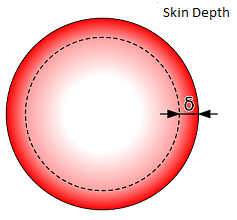
\includegraphics[scale=0.4]{Chapters/Chapter2/Flexible_PCB_coils/Figures/skin_depth.png} % TODO: Change image with svg
        \caption[Skin depth]{Representation of the thin surface generated by the skin effect}
        \label{fig: Skin_depth}
    \end{figure}

    The thickness of this area is called the \textbf{skin depth} and can be calculated using the formula
    \begin{equation*}
        \delta = \sqrt{\frac{\rho}{\mu \pi f}}
    \end{equation*}
            
    Where:
    \begin{itemize}
        \item \( \delta \) is the skin depth [m].
        \item \( \rho \) is the resistivity of the conductor [\(\Omega \cdot m\)].
        \item \( \mu \) is the magnetic permeability of the medium [H/m].
    \end{itemize}
    
    \begin{samepage}
        The effective resistance of the conductor can be derived from the skin depth using Dowell's equation \cite{AC_res_coils}
        \nopagebreak

        \begin{equation*}
            R_{skin} = F_{skin} \cdot R_{DC}
        \end{equation*}
        and
        \begin{equation*}
            F_{skin} = \frac{1}{2} (\frac{h}{\delta}) \frac{\sinh(\frac{h}{\delta}) + \sin(\frac{h}{\delta})}{\cosh(\frac{h}{\delta}) - \cos(\frac{h}{\delta})}
        \end{equation*}

        Where:
        \begin{itemize}
            \item \( R_{skin} \) is the effective resistance of the conductor due to the skin effect [\(\Omega\)].
            \item \( F_{skin} \) is the skin effect factor.
            \item \( h \) is the thickness of the conductor [m].
        \end{itemize}
    \end{samepage}

    \begin{samepage}
        In the case of the coil we're studying, the skin effect is \textbf{negligible} up to $1e8 Hz$ as the \textbf{thickness} of the flexible PCB's \textbf{traces} is \textbf{very low}.
        \nopagebreak

        \begin{figure}[H]
            \centering
            \includesvg[draft = false, width = 0.5\textwidth]{Chapters/Chapter2/Flexible_PCB_coils/Figures/Fskin_vs_freq.svg}
            \caption[Fskin of Flexar]{Logarithmic plot of the skin effect factor for a flexible PCB coil}
            \label{fig:Fskin of Flexar}
        \end{figure}
        \nopagebreak
    
        But we can observe from the study done on thicker traces' (0.5mm) coils that the skin effect starts to be already noticeable at $1e5 Hz$.
        \nopagebreak
        
        \begin{figure}[H]
            \centering
            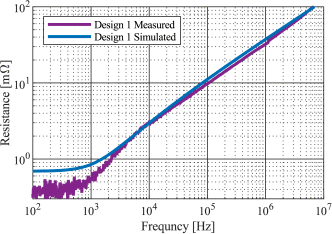
\includegraphics[width=0.5\columnwidth]{Chapters/Chapter2/Flexible_PCB_Coils/Figures/skin_effect_thicker.png}
            \caption[Skin effect on thicker traces]{Skin effect on thicker traces \cite{Sim_meas_AC_resistance_coils}}
            \label{fig: Skin_effect__thicker_trace}
        \end{figure}
    \end{samepage}

    \item \textbf{Proximity effect:} This effect is similar to the skin effect but it occurs when two conductors are close to each other. The current flowing through one conductor induces an \textbf{eddy current} in the other conductor which can lead to a change in the effective resistance of the conductors.
    
    \begin{figure}[H]
        \centering
        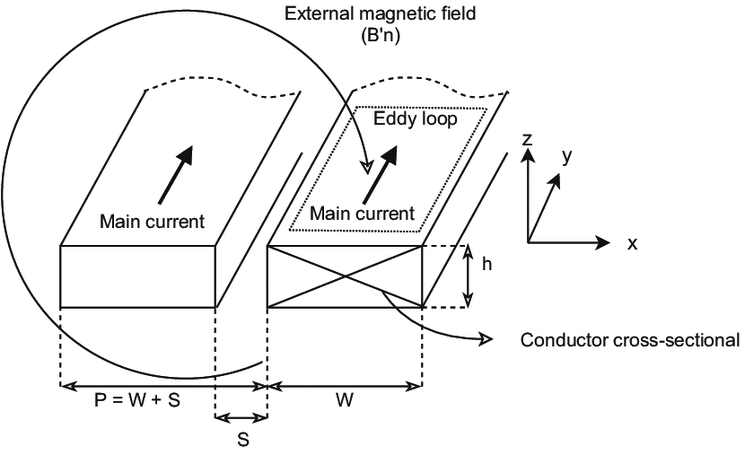
\includegraphics[width=0.4\columnwidth]{Chapters/Chapter2/Flexible_PCB_coils/Figures/proximity_effect.png}
        \caption[Proximity effect]{Representation of the proximity effect}
        \label{fig: Proximity_effect}
    \end{figure}

    \begin{samepage}
        The contribution of the proximity effect to the effective resistance of the coil can be calculated using the formula (considering current flowing in the coil $I_{ex} = 1A$) \cite{AC_res_Optimization}
        \nopagebreak

        \begin{equation*}
            R_{proximity} = \frac{1}{12} h \sigma \pi^2 f^2 B_n^2 w^3
        \end{equation*}
        \nopagebreak
        
        Where:
        \begin{itemize}
            \item \( \sigma \) is the conductivity of the conductor [\(\Omega^{-1} \cdot m^{-1}\)].
            \item \( h \) is the thickness of the conductor [m].
            \item \( f \) is the frequency of the AC current [Hz].
            \item \( B_n \) is the average external magnetic field [T].
            \item \( w \) is the width of the conductor [m].
        \end{itemize}
    \end{samepage}

    We can also approximate $F_{proximity}$ ($F_{proximity} = R_{proximity}/R_{DC}$) as
    \begin{equation*}
        F_{proximity} = \frac{F_{skin}}{3}
    \end{equation*}

    So when the contribution of the skin effect is negligible, the proximity effect will be \textbf{negligible} as well.

\end{itemize}







%----------------------------------------------------------------------------------------
%	SECTION 3
%----------------------------------------------------------------------------------------
\newpage
\section{Running PCB coils}\footnote{The \textit{"T81-558: Applications of Deep Neural Networks"} course of the Washington University \cite{T81-558} and the \textit{"CS231n: Deep Learning for Computer Vision"}\cite{CS231n} one are used as reference for the presentation of the topic.}
In the vast realm of artificial intelligence, a crucial discipline emerges: machine learning (ML), a transformative approach to programming that defies conventional code-based paradigms. At its essence, machine learning empowers systems to evolve and improve through experiences, learning patterns from data rather than relying on explicit instructions. This paradigm shift opens the door to a new era of problem-solving, where algorithms become adept at making decisions, predictions, and inferences based on the information they ingest.

\begin{figure}[th]
    \centering
    \includegraphics[scale=0.4]{Figures/Chapter2/Timeline-of-AI-to-Deep-Learning.png}
    \caption[Timeline of AI to Deep Learning.]{Timeline of AI toward Deep Learning.}
    \label{fig:TimelineAI}
\end{figure}

At the core of machine learning lies the intricate paradigm between algorithms and data. The learning process begins with a robust dataset, a collection of input features paired with corresponding outcomes. This data serves as the fodder for ML algorithms, mathematical constructs that decode patterns and relationships within the information. As the algorithm processes the data, it continually adjusts its internal parameters to better align its predictions with the ground truth.

Machine learning encompasses various learning paradigms, each tailored to specific challenges. In supervised learning, algorithms learn from labeled data, associating inputs with desired outputs. Unsupervised learning tackles unlabeled data, seeking inherent structures and relationships. Reinforcement learning introduces the element of interaction, where algorithms learn through trial and error, navigating an environment and adapting based on feedback.

As the capabilities of machine learning burgeoned, a more specialized branch emerged: deep learning. This paradigm shift brought about the rise of deep neural networks, inspired by the complexity of the human brain. Deep learning algorithms, structured as multi-layered neural networks, exhibit an unparalleled ability to automatically learn hierarchical representations from data.

Within the deep learning framework, neural networks delve into the intricacies of feature learning. These models, often identified as deep neural networks, boast multiple layers that autonomously extract increasingly complex features. The depth of these networks empowers them to uncover intricate patterns, making them particularly effective in tasks such as image and speech recognition.

The training process in machine learning and deep learning involves an iterative refinement of models. Algorithms, armed with backpropagation mechanisms, fine-tune their internal parameters to minimize the discrepancy between predicted and actual outcomes. This continual optimization results in models that not only perform well on training data but also generalize effectively to new, unseen data.

The applications of machine learning and deep learning span a multitude of domains, reshaping the landscape of technology and problem-solving. From image and speech recognition to natural language processing and autonomous systems, these methodologies have demonstrated unprecedented success. As we delve into the intricacies of machine learning and explore the depths of deep learning, we uncover the transformative power of algorithms that learn, adapt, and redefine the boundaries of artificial intelligence.
% -- Subsection 4.1
\subsection{High current needs}
The neural network is one of the first deep learning model. It emulates how neurons function in the human brain using connected circuits to simulate the intelligent behaviour.\\
Neural networks accept as input a feature vector with fixed length and produces as output a vector of predicted values with fixed length as well. Usually changing the input or output vector length means redesigning the entire structure.\\
The term \textit{"vector"} is usually referred to 1D arrays but with modern neural network it is increasingly common to find multiple dimensions arrays (as I will discuss later with the CNN).\\
The term \textit{"dimension"} can be misleading in neural networks, since, used in sense of the dimension of a vector, it refers to the number of elements present in that vector (for instance, a neural network with ten input neurons has ten dimensions). However, in the case of CNN the input has multiple dimensions, so 2D input to a neural network with 128x128 pixels leads to a configuration of 16,368 input neurons. In the first example the neural network will be defined as 2D NN, in the second one 16,368D.

\begin{figure}[th]
    \centering
    \includegraphics{Figures/Chapter2/NeuralNetwork.jpg}
    \caption[Neural Network]{Neural Network's layer representation.}
    \label{fig:NeuralNetwork}
\end{figure}

% -- Subsection 4.2
\subsection{Costant voltage vs current power supply}
The neural network can functions in regression or classification. In the first case the output is a number predicted on the base of the input data, in the second one the identification of a specific class o category. It is important to note that the output of a regression or two-class classification model is a number (binary for the classification 1 for true value 0 or -1 for false value), but in case of multi-class classification the neural network has an output neuron for each category. 

% -- Subsection 4.3
\subsection{Difference between DC and AC signals}
The artificial neuron receives as input one or more sources from input data or previous layer neurons. It multiplies each of those inputs by a respective weight and sums these multiplications together (sometimes also a bias factor is added). The result is passed to an activation function that determines the output of the neuron.\\
\begin{equation}
    f(x,w) = \phi(\sum_i(w_i\*x_i))
\end{equation}

In the above equation the variables \textit{x} and \textit{w} represent the input and the weights of the neuron respectively, the \(\phi(\cdot)\) the activation function and \textit{f(x,w)} the output of the neuron.

\begin{figure}[th]
    \centering
    \includegraphics[scale=0.6]{Figures/Chapter2/Neuron.jpg}
    \caption[Neuron]{Artificial Neuron representation.}
    \label{fig:Neuron}
\end{figure}

The neurons can be classified in four categories, depending on their position in the architecture:
\begin{itemize}
    \item\textbf{Input Neurons:} each input neuron is mapped to an element in the feature vector.
    \item\textbf{Hidden Neurons:} intermediate neurons responsible of the abstraction of the neural networks to process the input into the output.
    \item\textbf{Output Neurons:} each output neuron calculates one part of the output.
    \item\textbf{Bias Neurons:} introduces an additional learnable parameter that improves the prediction's accuracy by shifting the activation threshold on the activation function.
\end{itemize}

\subsection{AC polarized signals}

\subsubsection{Need for low RMS signals}
Activation functions, or transfer functions, have the role of computing the output of each layer of a neural network. Historically the more common are hyperbolic tangent, sigmoid, or linear activation functions. However, with modern deep learning models, specialized activation functions have been introduced to suit specific applications and tasks:
\begin{itemize}
    \item\textbf{Rectified Linear Unit (ReLU):} use for the output hidden layers.
    \item\textbf{Softmax:} used for the output of classification neural networks.
    \item\textbf{Linear:} used for the output of regression neural networks.
\end{itemize}
In particular ReLU has gained rapid popularity in deep learning due to its ability to yield superior training results. Before the era of deep learning, the sigmoid function was the most prevalent activation function. However, as modern frameworks like PyTorch frequently train neural network using gradient descent optimization, computing partial derivatives of the sigmoid became a computationally challenging operation. The introduction of the Rectified Linear Unit significantly simplified this computation leading to improved performance and faster training.

\begin{figure}[th]
    \centering
    \includegraphics[scale=0.4]{Figures/Chapter2/ActivationFunctions.png}
    \caption[Sigmoid vs. ReLU]{Sigmoid and ReLU activation functions graphic representation.}
    \label{fig:ActivationFunctions}
\end{figure}

%-----------------------------------
%	SUBSECTION 2
%-----------------------------------

%\subsection{Convolutional Neural Network (CNN)}
The Convolutional Neural Network (CNN) is a neural network technology that has deeply impacted the area of computer vision. The original concept of a CNN was introduced by Fukushima in 1980\parencite{fukushima} and subsequent significant advancements were made by LeCun \emph{et al.}\parencite{Lecun}.

\begin{figure}[th]
    \centering
    \includegraphics[scale=0.4]{Figures/Chapter2/CNN.png}
    \caption[Convolution Neural Network]{Convolutional Neural Network visual representation.}

    \label{fig:CNN}
\end{figure}
The CNN, in contrast with most neural networks, has a specific order of the input elements and it is crucial to the training. The inputs are arranged into a grid which represents the input image, the highest-level unit. On the other hand each pixel is the smallest unit within the image and represents a scalar value denoting the intensity or color at a specific location. The images can be colored (expressed on three channels RGB) or grayscale with a single channel.
Due to the amount of data, additional layers are needed to lighten the computation load. The layers works together to extract features from the input data and predict the output. The additional layers are:
\begin{itemize}
    \item\textbf{Convolutional Layers:} apply filters or kernels to perform convolution operations, extracting local features like edges and shapes.
    \item\textbf{Pooling Layers:} reduce the spacial dimensions of feature maps, making the network more robust to scale and orientation variation.
    \item\textbf{Dense Layers:} these layers connect all neurons to every neuron in the previous and subsequent layers, performing high-level feature extraction and decision-making.
    \item\textbf{Flattening Layer:} reshape the output from convolutional layers to 1D vector, allowing it to connect to fully connected (dense) layers.
\end{itemize}

%\subsubsection{Training and Testing Processes}
The training process begins with the initialization of the network's weight and biases; usually these parameters are set to small random values.\\
The input is then fed through the network, the data propagates through each layer and predictions are produced. A loss function is used to quantify the error between the predicted and the ground truth values. The choice of the loss function depends on the specific task, the most common are MSE for regression and cross-entropy for classification. The backpropagation algorithm is employed to compute the gradients of the loss with respect to the network's parameters (weights and biases).\\
This process is essentially the chain rule from calculus, which calculates how small changes in each parameter affect the loss. Using the gradients computed during backpropagation, the network's weights and biases are updated through an optimization algorithm.

The goal is to adjust the parameters in a way that minimizes the loss function. The process is then iterated over the entire training dataset with a process called epoch. Multiple epochs are typically performed to improve the model's performance.

Periodically, the model's performance is evaluated on a separated validation dataset that the network has not seen during training. This method helps monitor the model's generalization capabilities.

After training and validation, the model is tested on a completely unseen test dataset to evaluate its performance on new, independent data.

%----------------------------------------------------------------------------------------
%	SECTION 4
%----------------------------------------------------------------------------------------
\section{Coil-Magnet-Membrane system}\footnote{The \textit{"T81-558: Applications of Deep Neural Networks"} course of the Washington University \cite{T81-558} and the \textit{"CS231n: Deep Learning for Computer Vision"}\cite{CS231n} one are used as reference for the presentation of the topic.}

% -- Subsection 5.1
\subsection{Neodynium magnets (magnetic strenght wrt class and dimensions)}

% -- Subsection 5.2
\subsection{Magnetic "coupling" between magnet and coil}

\subsubsection{Relation between coil and magnet diameter}

\subsubsection{Distance between coil and magnet}

% -- Subsection 5.3
\subsection{Membrane-Magnetsystem}

%----------------------------------------------------------------------------------------
%	SECTION 5
%----------------------------------------------------------------------------------------
\section{Membrane-Finger haptic system}
 
% Chapter Template

\chapter{Overview of Haptic Feedback} % Main chapter title

\label{Chapter3}

Haptic Feedback or Haptics, in short, is the research field that deals with the need to be able to \textbf{digitalize the human sense of touch and reproduce it}. Despite the research done in this field since the mid-20\textsuperscript{th} century, the technology is still in its infancy. The main reason for this is the \textbf{complexity of the human sense of touch} which we still don't understand fully.
This, in turn, doesn't allow us to even approximately match the capabilities of the human sense of touch; but we can still use this infant technology to reproduce \textbf{simple sensations}.
Simple sensation reproduction can still be used in many fields, from the \textbf{entertainment} industry to the \textbf{medical field}, from the \textbf{military} to the \textbf{automotive industry} to \textbf{convey information that we do not normally acquire via touch}, such as notifications and warnings related to particular events, guidance instructions, and even crude reproduction of textures.
In this chapter, we will give an overview of the human sense of touch and the state of art technologies used to reproduce it.

%----------------------------------------------------------------------------------------
%	SECTION 1
%----------------------------------------------------------------------------------------
\section{Physics of Haptic Feedback}
\label{Introduction_Haptics}


% -- Subsection 1
\subsection{Biology of Haptic Sensing}
The human tactile sensing system can measure specific properties of materials, such as
temperature, texture, shape, force, fine-form features, mass distribution, friction, hardness
and viscoelasticity, through physical contact between the human skin and the object.
Even the changing state of the interaction, such as gravitational and inertial effects, can
be perceived through the sense of touch. 
As the sensing system works through the skin, it doesn't rely on a localized sensory organ but behaves as a distributed system, also different parts of the body have different thresholds of sensitivity.
For these reasons, it's difficult to treat a tactile signal as a well-defined quantity like visual and
audio signals and its complex nature makes it difficult to replicate its functioning in
science or engineering tasks.

The sense of touch is based on the somatosensory system, which is a complex system of nerve endings and touch receptors in the skin. The somatosensory system is composed of four main types of receptors:
\begin{itemize}
    \item \textbf{Mechanoreceptors} - These are the most common type of tactile receptors in the skin. They are responsible for sensing pressure, vibration, stretching, and brushing.
    \item \textbf{Thermoreceptors} - These receptors are responsible for sensing temperature changes in the skin. There are two main types of thermoreceptors: warm receptors and cold receptors.
    \item \textbf{Nociceptors} - These receptors are responsible for sensing pain and tissue damage. They are activated by noxious stimuli, such as extreme temperatures, pressure, or chemicals.
    \item \textbf{Proprioceptors} - These receptors are responsible for sensing the position and movement of the body. They are located in the muscles, tendons, and joints, and provide feedback to the brain about the relative position between different parts of the body.
\end{itemize}

The most important receptors for haptic feedback are the mechanoreceptors, they react to mechanical stimuli by producing signals in the form of streams of voltage pulses at high frequencies, the stronger the stimuli higher the frequency of the pulses. When the cell adapts to the stimulus, the pulse frequency subsides to its normal rate.
Considering the goal of this research we can focus on the mechanoreceptors that are responsible for sensing pressure and vibration, these are the Pacinian corpuscles and the Meissner corpuscles.
The first ones are more sensible to high-frequency vibrations (200-550Hz), while the second ones are more for low-frequency vibrations (20-40Hz). \cite{Alg_Wearable_Tech_Nicole}

% -- Subsection 2
\subsection{Haptic sensitivity}
\label{Haptic sensitivity}

As the mechanoreceptors are \textbf{enveloped in various skin layers}, their sensitivity to vibrations will not be infinite. The \textbf{strength of the sensation} will depend on the \textbf{frequency} and \textbf{amplitude of the vibration}. 

The \textbf{amplitude} of the vibration can be considered in \textbf{terms of the acceleration of the membrane-magnet system}.

Previous works \cite{Vibrotactile_Sensitivity} found that, for a pulp contact area ranging from 53 to 176.7 mm\textsuperscript{2}, the threshold of detection of vibrations was between 0.1778 and 0.5623 m/s\textsuperscript{2} (in the work specified as 105-115 dB (re 1e-6m/s\textsuperscript{2})) for sinusoidal stimuli ranging from 100 to 250 Hz. 
For frequencies close to \textbf{125Hz} the threshold should also \textbf{lower} as the finger pulp reaches its \textbf{resonance frequency} \cite{Skin_freqs_penetration}.

The study also highlights that the sensitivity depends on the \textbf{constant pressure force applied on the skin} in conjunction with the vibration.
They found that under active pressing force, the sensitivity threshold decreases to 0.027-0.143 m/s\textsuperscript{2} (in the work specified as 68.5-83.1 dB (re 1e-6m/s\textsuperscript{2})) for a constant applied force of 1.6N.

\begin{samepage}
    For higher pressure forces the sensitivity threshold decreases even further, as we can observe in Fig. \ref{fig: Vibrotactile_Sensitivity}.
    \begin{figure}[H]
        \centering
        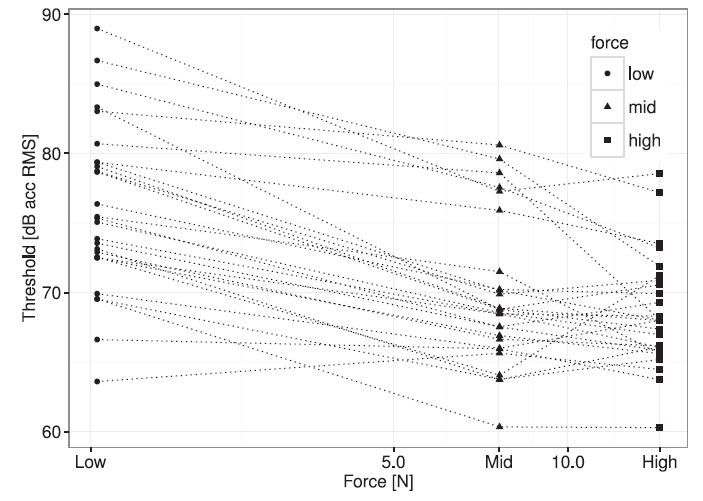
\includegraphics[width=0.5\linewidth]{Chapters/Chapter3/Haptics_Physics/Figures/vibr_thr_vs_pressure_force.png}
        \caption{Sensitivity as a function of the applied pressure \cite{Skin_freqs_penetration}.}
        \label{fig: Vibrotactile_Sensitivity}
    \end{figure}
\end{samepage}



%----------------------------------------------------------------------------------------
%	SECTION 2
%----------------------------------------------------------------------------------------
\section{State of the Art in vibrotactile haptic feedback}
For now, state of the art in haptic feedback is still in its infancy.
The main reason for this is the complexity of the human sense of touch which we still don't understand fully.
The \textbf{best technology} we have for now to reproduce haptic feedback through \textbf{vibrotactile} means is the \textbf{piezoelectric actuator}.

% --- SUBSECTION 1
\subsection{Piezoelectric actuators}
Piezoelectric actuators are a very interesting technology based on the \textbf{piezoelectric effect}.
Materials exhibiting this effect, such as certain ceramics and crystals, possess the ability to \textbf{convert electrical energy into mechanical motion}, and vice versa.

The operating principle of piezoelectric actuators relies on the application of an electric field across the piezoelectric material. This electric field induces a \textbf{deformation within the material}, causing it to expand or contract depending on the polarity of the applied voltage. This minute deformation translates into \textbf{highly precise mechanical displacement}, enabling piezoelectric actuators to achieve nanometer-scale resolutions with \textbf{remarkable speed and accuracy}.

One of the defining characteristics of piezoelectric actuators is their \textbf{rapid response time}. Unlike traditional electromagnetic actuators, which may suffer from inertia and mechanical backlash, piezoelectric actuators can swiftly change their state in response to electrical signals.

\subsubsection{Frequency response}
Piezoelectric actuators are perfect for haptic applications as they can provide a \textbf{wide range of frequencies}.
Piezo specifically engineered for haptic feedback can provide a frequency range from 1 Hz to 1 kHz. \\

All piezoelectric actuators have a natural frequency at which they resonate. This \textbf{frequency} is determined by the \textbf{mechanical properties} of the actuator, such as its mass and stiffness, as well as the electrical properties of the piezoelectric material.

\begin{samepage}
    The important thing to note is that this \textbf{frequency also depends on the load} that the actuator is driving:
    \nopagebreak

    \begin{equation}
        f_{res} = \frac{1}{2\pi} \sqrt{\frac{k}{m_{eff}+m_{load}}}
    \end{equation}
    \nopagebreak

    Where:
    \nopagebreak

    \begin{itemize}
        \item \( f_{res} \) = Resonant frequency [Hz]
        \item \( k \) = Stiffness of the piezo actuator [N/m]
        \item \( m_{eff} \) = Effective mass of the actuator [kg]
        \item \( m_{load} \) = Mass of the load [kg]
    \end{itemize}
\end{samepage}


As the frequency of the actuator approaches its resonant frequency, the \textbf{amplitude} of the actuator's motion \textbf{increases significantly}. This phenomenon must be taken into account when designing a control system for the piezo actuator, as at maximum voltage the actuator could be \textbf{damaged} if in resonance.

\subsubsection{Force performances}
Taking as an example a piezo actuator built specifically for haptic feedback, the PowerHap series from TDK \cite{Piezo_Haptic_Actuator}, we can see that the actuator can provide a force up to \textbf{20N} in a frequency range from 1 Hz to 500Hz.

\subsubsection{Power consumption}
Considering still as an example the PowerHap series from TDK, we can read from the datasheet that the actuator can be run with a peak voltage of 120V and an average current of 0.432A (calculated using \cite{Power_piezo_calculator} in the case of a square wave signal of 500Hz). This means that the actuator can \textbf{consume} up to \textbf{25.9W} of power at its peak frequency.
In the same condition, it will also \textbf{dissipate} about \textbf{2.59W} of power as heat.

% % --- SUBSECTION 2
\subsection{Texture rendering} % TODO: Decide if this section is needed
\begin{itemize}
    \item frequency requirements
    \item force requirements
    \item response time
\end{itemize}



%----------------------------------------------------------------------------------------
%	SECTION 4
%----------------------------------------------------------------------------------------
%\section{Performance comparison between Piezo and Coil's actuators}

% % -- Subsection 2.1
% \subsection{Force and displacement}

% % -- Subsubsection 2.2
% \subsection{Frequency response} %TODO: decide if to include this section
% Chapter Template

\chapter{Powering circuit design} % Main chapter title
\label{Chapter4}
In this chapter, we will present some of the engineering challenges faced during the design of a power circuit for our flexible voice coil actuator.
We will mostly describe an ideal circuit as we will later demonstrate that running this actuator would require very advanced analog circuitry, comprised of high-cost components.
Most of the tests we will present have been done using a bench signal generator and amplifier.

%----------------------------------------------------------------------------------------
%	SECTION 1
%----------------------------------------------------------------------------------------
\section{Power Circuit Block diagram}
The power circuit can be summarized as a block diagram, as shown in figure \ref{fig:Power_Circuit_Block_Diagram}.
\begin{figure}[H]
    \centering
    \resizebox{.9\linewidth}{!}{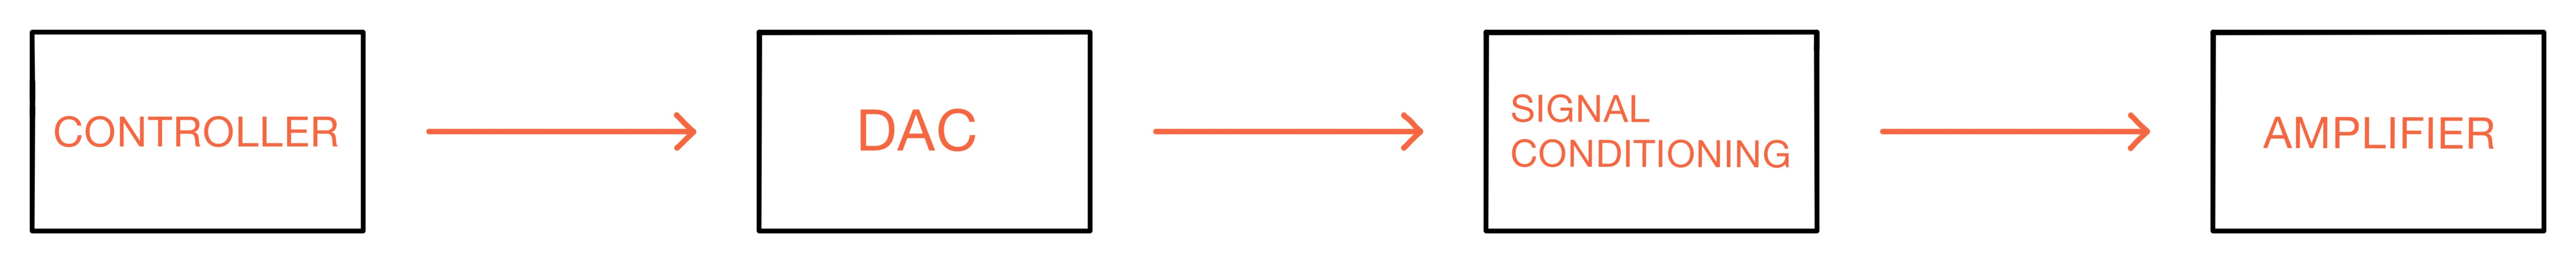
\includegraphics{Chapters/Chapter4/Figures/power_circuit_block_diagram.jpg}} % TODO: sostituire con svg
    \caption{Block diagram of the power circuit.}
    \label{fig:Power_Circuit_Block_Diagram}    
\end{figure}

%----------------------------------------------------------------------------------------
%	SECTION 2
%----------------------------------------------------------------------------------------
\section{Controller}
The controller in this application has to be a \textbf{signal generator} that can produce a waveform that can be amplified and sent to the coil.
The controller we used for testing is an ESP32 microcontroller.
We chose this controller as the first test hardware for its \textbf{simplicity of programming} and its \textbf{integrated DAC}.

% -- Subsection 4.1
\subsection{ESP32 DAC Characteristics}
The DAC included in the ESP32 is a pretty basic one but as a first test, it is enough.
The DAC has a resolution of \textbf{8 bits}, and it can output a voltage between \textbf{0} and \textbf{3.3V} with a maximum current output of \textbf{12mA}.

\subsection{ESP32 waveform generator}
Using a simple program the ESP32 can be used as a pretty capable waveform generator.
The software we used is the \textbf{ESP32 Signal Generator} from \textbf{\href{https://corz.org}{corz.org}} \cite{corz_signal_gen}.
This software allows the user to generate the following waveforms:
\begin{itemize}
    \item Sine wave from 16Hz to 500kHz
    \item Square wave from 1Hz to 40MHz
    \item Triangle wave from 153Hz to 150kHz 
    \item Sawtooth wave from 153Hz to 150kHz
\end{itemize}

\begin{samepage}
    Between these ranges of frequencies, the generated waveforms are pretty accurate.
    \nopagebreak

    \begin{figure}[H]
        \centering
        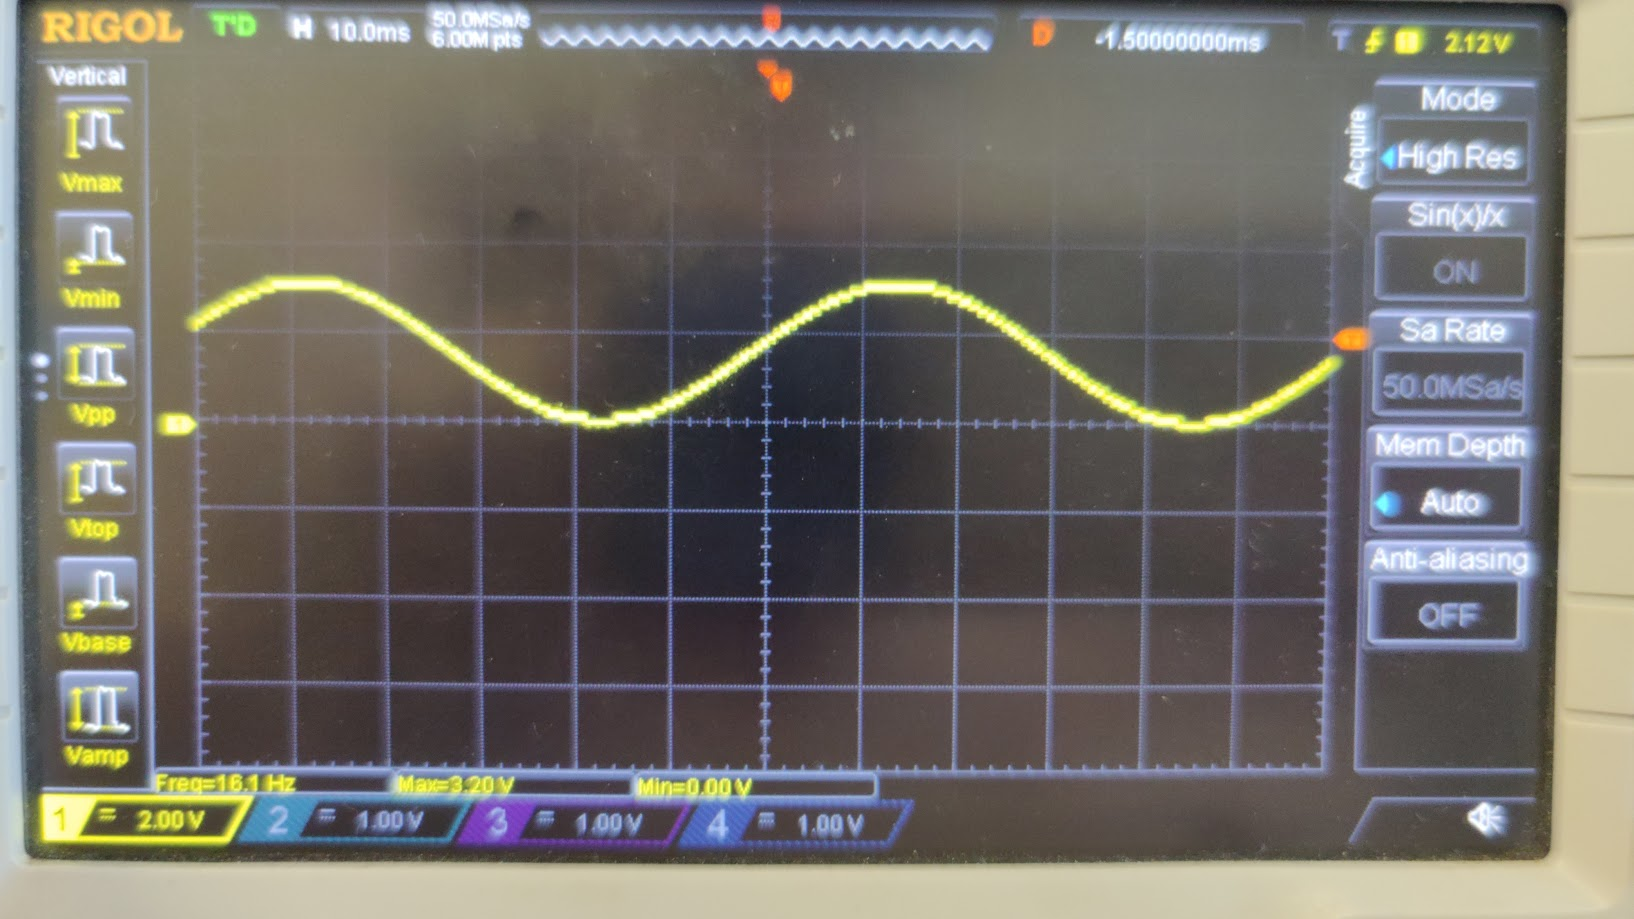
\includegraphics[width=0.9\linewidth]{Chapters/Chapter4/Figures/16Hz_signal_gen.jpg}
        \caption[ESP32 DAC in action]{ESP32 16Hz Sine wave generated by the ESP32 Signal Generator software.}
        \label{fig:16Hz_signal_gen}
    \end{figure}
\end{samepage}

\pagebreak

% \subsubsection{Esp32 DAC limitations}

% \subsubsection{Esp32 DAC Noise}

The controller we used for testing is an ESP32 microcontroller.
We chose this controller for the simplicity of programming and the integrated DAC.
%----------------------------------------------------------------------------------------
%	SECTION 3
%----------------------------------------------------------------------------------------
\section{Signal Conditioning Circuit}
\label{Signal_Conditioning_Circuit}
We know that the controller DAC \textbf{outputs a voltage} between \textbf{0} and \textbf{3.3V}, the power stage has a \textbf{gain of 10}, and that to drive Flexar's coils, at their rated \textbf{maximum power of 0.8W}, we need to provide a voltage of about \textbf{6V} at a current of \textbf{0.2A}. \\
A very simple solution is to implement a \textbf{variable voltage divider} to adjust the amplitude of the signal coming from the DAC.

\begin{samepage}
    We chose a \textbf{maximum dividing factor of 10} to match the power stage gain.
    \nopagebreak

    \begin{figure}[H]
        \centering
        \resizebox{.5\linewidth}{!}{\begin{circuitikz}[american]
    \draw (0,0) node[ground]{} to[sV, l=$V_{DAC}$] (0,3) to[vR, l=$R_1$] (3,3) to[R, l=$R_2$] (3,0) node[ground]{};
    \draw (3,3) to[short, -o] (4,3) node[right]{$V_{out}$};
\end{circuitikz}}
        \caption{Signal conditioning circuit.}
        \label{fig:cond_circuit}
    \end{figure}
    \nopagebreak

    Where:
    \nopagebreak

    \begin{itemize}
        \item $V_{DAC}$ is the voltage coming from the controller DAC [0,3.3]V.
        \item $R_1$ is a 100$k\Omega$ potentiometer to adjust the amplitude of the signal.
        \item $R_2$ is a 10$k\Omega$ resistor to set the maximum amplitude of the signal.
        \item $V_{out}$ is the output voltage of the conditioning circuit [0, 0.33]V.
    \end{itemize}
\end{samepage}

The output voltage of the conditioning circuit is given by the following formula:
\begin{equation}
    V_{out} = V_{DAC} \cdot \frac{R_1}{R_1 + R_2}
\end{equation}

The values of $R_1$ and $R_2$ have been chosen to be 100$k\Omega$ and 10$k\Omega$ respectively, as they are standard values, provide a good range of adjustment for the amplitude of the signal, and their order is \textbf{big enough} to work with the provided DAC current of 12mA.

%----------------------------------------------------------------------------------------
%	SECTION 4
%----------------------------------------------------------------------------------------
\section{Amplifier circuit}
The online architecture operates in real-time. It processes the input data from the camera and produces as output the satellite pose estimation.

After being pre-processed, the image captured from the camera is passed to the \textit{Landmark regression} module. The latter predicts the 2D location \{\(\textbf{z}_i\)\} of the 9 landmarks along with the visibility coefficient \{\(v_i\)\} for each of them. The \textit{Landmark Mapping} module then uses these data to compute the 3D position of each landmark with respect to the camera frame. The final 6DOF pose of the satellite is then computed from the CPD module. Figure \textbf{\ref{fig:Online Pipeline}} shows the online pipeline of the implemented methodology.
\begin{figure}[H]
    \centering
    \includegraphics[scale=0.6]{Figures/Chapter4/Online Pipeline.png}
    \caption[Online pipeline of the implemented pose estimator.]{Online pipeline of the implemented pose estimator.}
    \label{fig:Online Pipeline}
\end{figure}

% -- Subsection 2.1
\subsection{High Power Operational Amplifiers}
\label{Chapter4/Pre-Processing}
The image captured from the camera is pre-processed in the \textit{Pre-Processing} module. It consists in a bilateral filter, which is a non-linear, edge-preserving smoothing filter that reduces noise while preserving the edges in an image.\\
The mathematical steps behind the bilateral filter involve computing weighted averages of pixel values within a local neighborhood. 
\begin{figure}[th]
    \centering
    \includegraphics[scale=0.32]{Figures/Chapter4/bilateral_filtering.png}
    \caption[Bilateral Filter.]{Bilateral Filter mathematical steps.}
    \label{fig:Bilateral Filter}
\end{figure}

The formula for the bilateral filter operation can be described as follows:

Given an input image \(I(x, y)\) and the filter parameters:
\begin{itemize}
    \item \(d\) (diameter of each pixel's neighborhood)
    \item \(\sigma_c\) (standard deviation of the color space)
    \item \(\sigma_s\) (standard deviation of the spatial space)
\end{itemize}
The filtered output image \(B(x, y)\) can be computed using the following equation for each pixel \((x, y)\):
\begin{equation}
   B(x, y) = \frac{1}{W(x, y)} \sum_{(i, j) \in S} I(i, j) \cdot G_c(I(x, y), I(i, j), \sigma_c) \cdot G_s(x, y, i, j, \sigma_s) 
\end{equation}


Where:
\begin{itemize}
    \item \(S\) is the neighborhood of pixel \((x, y)\), defined by a window of diameter \(d\).
    \item \(G_c\) is the color similarity term, which measures the similarity in color between pixels \((x, y)\) and \((i, j)\) in the color space.
    \item \(G_s\) is the spatial similarity term, which measures the spatial proximity between pixels \((x, y)\) and \((i, j)\).
    \item \(W(x, y)\) is a normalization factor.
\end{itemize}
The \(G_c\) term is defined as a Gaussian function in the color space:
\begin{equation}
    G_c(I(x, y), I(i, j), \sigma_c) = \exp\left(-\frac{\|I(x, y) - I(i, j)\|^2}{2\sigma_c^2}\right)
\end{equation}

The \(G_s\) term is a Gaussian function in the spatial space:
\begin{equation}
    G_s(x, y, i, j, \sigma_s) = \exp\left(-\frac{\|(x, y) - (i, j)\|^2}{2\sigma_s^2}\right)
\end{equation}

\begin{figure}[th]
    \centering
    \includegraphics[scale=0.5]{Figures/Chapter4/Pre-processing.png}
    \caption[Input and pre-processed image.]{On the left the original sample image from the training dataset, on the right the resultant image after the application of the bilaterial filter ($d = 40,\sigma_c = 40,\sigma_s = 200$).}
    \label{fig:Pre-processing}
\end{figure}

The bilateral filter operates by applying these Gaussian weighting functions to compute the weighted average of pixel values within the defined neighborhood, both in color and spatial spaces, resulting in a smoothed image that preserves edges and details. The filter helps reduce noise while keeping the important structures in the image intact.

\subsubsection{Old type of op-amp}
\subsubsection{Power dissipation problems}

% -- Subsection 2.2
\subsection{High Power Voltage Amplifier}
\label{Chapter4/CPD}
As the \textit{Landmark Mapping} module predicts the position of each landmark independently one from the other and so each landmark has its own error over the three axis, the resultant cloud of points is misaligned with respect to the rigid reference position given by the CAD model.\\
In order to estimate the 6DOF pose of the satellite and in the meantime overcome this misalignment problem a mathematical technique is used: Coherent Point Drift.

Two sets of 3D points are present: one is the "target", which represents the 3D position of the landmarks in the camera frame supposing no translation and no rotation, and the other is "source", which is the 3D position of the predicted landmarks.
The "source" point set is only composed by landmarks identified in the image frame (\(v_i = 1\)). It is important to know that the algorithm's performances strongly depend on the number of points in the set so, with the camera approaching the target, some landmarks are cut from the image frame and consequently the pose estimation accuracy reduces.

\begin{figure}[H]
    \centering
    \includegraphics[scale=0.23]{Figures/Chapter4/CPD.png}
    \caption[Iterations of the CPD optimization process.]{Iterations of the CPD optimization process.}
    \label{fig:CPD}
\end{figure}

%----------------------------------------------------------------------------------------
%	SECTION 5
%----------------------------------------------------------------------------------------
\section{Power Supply}

%----------------------------------------------------------------------------------------
%	SECTION 6
%----------------------------------------------------------------------------------------
\section{Implementation problems and possible alternatives}

% -- Subsection 5.1
\subsection{Non idealities}
\label{Chapter4/LandmarksSel}
The main problem in the implementation of the \textit{Landmark regression} module (\textbf{\ref{Chapter4/LandReg}}) is the selection of the landmarks.
Selecting meaningful landmarks is a critical first step, requiring a accurate understanding of the satellite's structure. These landmarks must possess distinct characteristics that remain invariant under varying conditions, such as changes in lighting, orientation, or potential occlusions.

The first performed attempt in the selection of the landmarks was composed of 11 landmarks with relevant features in the satellite's structure. Most of those visual features were similar to each others and the resultant heatmap predicted by the CNN for a single landmark was ambiguous among multiple ones. This led to a complicated recognition of the landmark location in the image with complex and heavier algorithms for the 2D position identification.

In both cases the set of landmarks has been selected near the approach target to limit the number of out of frame landmark in closer positions.

\subsubsection{Stability}

\subsubsection{Phase Shift}

\subsubsection{Noise}

% -- Subsection 5.2
\subsection{Polarized signals}

% -- Subsection 5.3
\subsection{Alternative Amplifiers}
\label{Chapter4/DatasetAv}
Another notable challenge stems from the limited size of available datasets. A smaller dataset poses a risk of overfitting, potentially hindering the model's ability to generalize across diverse scenarios. Addressing this issue requires careful consideration of data augmentation techniques, introducing various transformations to enhance the model's adaptability.

The dataset used for training present five different orientations on each axis of the satellite during the whole approaching range. The main limitation given by the used dataset is the lack of combined rotations over multiple axis and a wider range of rotation on single axis.

Even though the \textit{Landmark regression} module training is strictly related to the availability of the images, the \textit{Landmarks Mapping} one is totally independent. The 2D-3D correspondence of landmarks used to train the model requires the only relative position of the landmarks from the CAD Model and the perspective matrix to be performed. This means that a possible further step to expand the dataset is to perform several simulations with rotations over multiple axis to create new wider datasets and improve the model performances.

\subsubsection{Current Amplifiers}

 
% Chapter Template

\chapter{Implementation and Prototypes} % Main chapter title

\label{Chapter5}

%----------------------------------------------------------------------------------------
%	SECTION 1
%----------------------------------------------------------------------------------------
\section{Rigid Prototypes}
The goal of this research is to develop a flexible device, but before delving into flexible prototypes we started by designing some rigid ones. The rigid prototypes were designed to test the concept of this device and to understand the \textbf{limitations} of the technology.

% -- Subsection 2.1
\subsection{1st version - Dresda Coils testbed}
The first prototype was designed to test the capabilities of the Dresden coils.
In the previous research done by the HZDR team \cite{HZDR} they tested the coil using a simple piece of \textbf{flexible magnetic tape as a membrane}.

\subsubsection{Flexible magnetic membrane}
\begin{samepage}
    This membrane is shaped like a "fish" so the tail can be fixed on a plane and the head can be \textbf{free to bend} up and down (as seen in Fig.\ref{fig: Dresden_test}).
    \nopagebreak

    \begin{figure}[H]
        \centering
        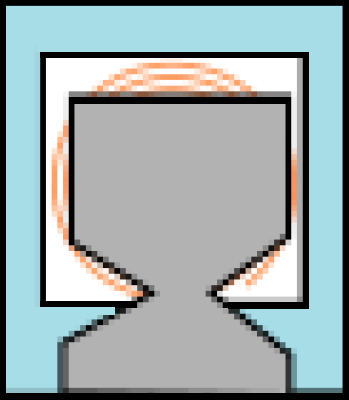
\includegraphics[width = 0.2\linewidth]{Chapters/Chapter5/Rigid_Prototypes/Figures/Dresden_test.png}
        \caption{Dresden coil HZDR test setup}
        \label{fig: Dresden_test}
    \end{figure}
\end{samepage}

When the coil is powered, the magnetic field produced by the coil repels the membrane and bends it up.
The coil would be powered with an \textbf{AC signal} at various frequencies, then one would need to keep his pulp \textbf{suspended} at a certain distance over the membrane and feel the vibration produced by the membrane.
The pulp needed to be suspended at a certain distance to \textbf{avoid pressing} on the membrane, this would have caused the membrane to \textbf{stop vibrating}.

\subsubsection{Adjustable height platform for coil and membrane}
The most important thing to solve was to find a way to keep the pulp at a certain distance from the membrane.

\begin{samepage}
    Firstly we designed a platform that could keep the finger steady.
    \nopagebreak

    \begin{figure}[H]
        \centering
        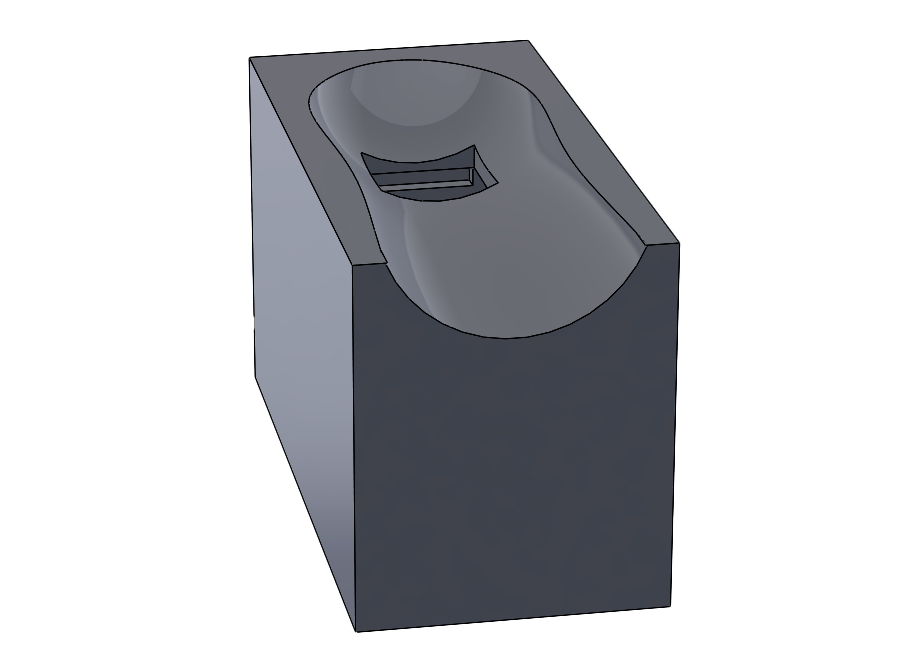
\includegraphics[width=0.5\linewidth]{Chapters/Chapter5/Rigid_Prototypes/Figures/finger_holder.png}
        \caption{Finger platform}
        \label{fig: finger_platform}
    \end{figure}
\end{samepage}

This platform was modeled to have an \textbf{ergonomic} cavity for the finger to rest in and a hole for the pulp to be suspended over the membrane.
The square hole is large enough to allow the "fish" membrane to move \textbf{freely}.
Under the hole, there is a large cavity where a mechanism is placed.
This mechanism is a platform where the coil and membrane can be placed in a configuration similar to the one used in the HZDR experiment.
The platform can then be \textbf{raised or lowered} to find the right distance between the membrane and the finger pulp.
\begin{figure}[H]
    \centering
    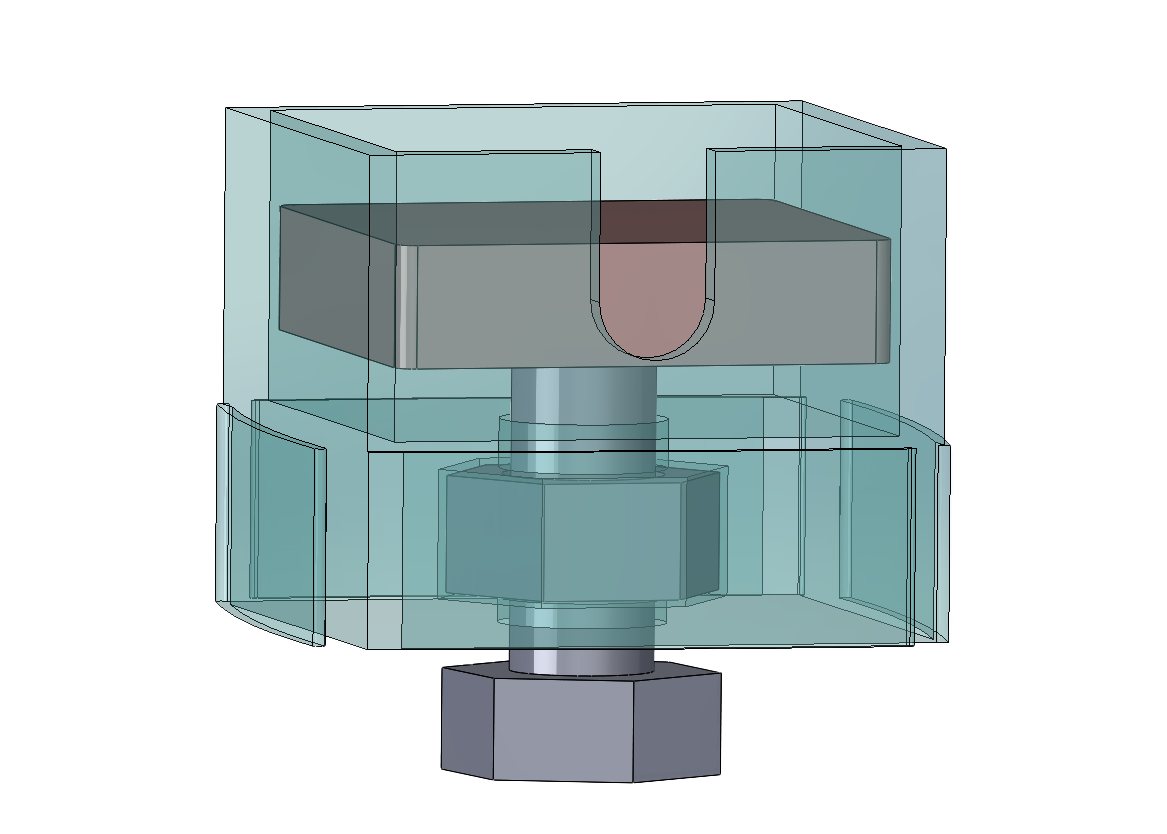
\includegraphics[width = 0.5\linewidth]{Chapters/Chapter5/Rigid_Prototypes/Figures/adj_platform.png}
    \caption{Adjustable platform}
    \label{fig: adj_platform}
\end{figure}
The mechanism is a simple screw that can be turned to raise or lower the platform, which is laying on top of it.

\subsubsection{Prototype usability}
This prototype proved to be pretty \textbf{difficult} to use.
The main problem was that distance couldn't be easily adjusted as the platform wouldn't remain \textbf{stable enough} on the screw.
This meant that finding an optimal distance between the pulp and the membrane was difficult, especially because different people have \textbf{different pulp thicknesses}.
Even if a distance that was good for one person was found, the vibration produced by the membrane was \textbf{very weak} and could barely be felt.

% -- Subsection 2.2
\subsection{Wearable Rigid Prototypes}
With this prototype, we wanted to try \textbf{fixing most of the problems} encountered with the previous prototype.

Firstly we decided to substitute the Dresden coil with the Flexar one as it was more powerful.
Then we wanted to \textbf{decouple the membrane} from the coil to prevent the membrane from being pressed by the pulp and remove the need for an adjustable platform to keep the coil at the right distance.
Finally, we wanted to make the device \textbf{wearable}.

\subsubsection{Finger-Membrane interface}
After some testing, we found that a good way to decouple the membrane from the coil and better the transmission of vibrations to the finger was to use a small \textbf{high-performance magnet} attached directly to the finger pulp.

For our testing, we used an \textbf{N42-grade} neodymium cylindrical magnet with a diameter of \textbf{10mm} and a height of \textbf{3mm}.
This magnet was \textbf{fixed} to the index pulp of the tester using some non-toxic glue and then he would be able to feel substantial vibrations by moving his pulp closer to the powered-on coil (with an AC signal).

Considering this knowledge, we designed a \textbf{silicon sleeve} that could be \textbf{worn} on the finger, this sleeve has a cavity for the magnet to be inserted into and be kept \textbf{near the skin}.

\begin{figure}[H]
    \centering
    \resizebox{1\textwidth}{!}{
        \begin{subfigure}[b]{0.6\textwidth}
            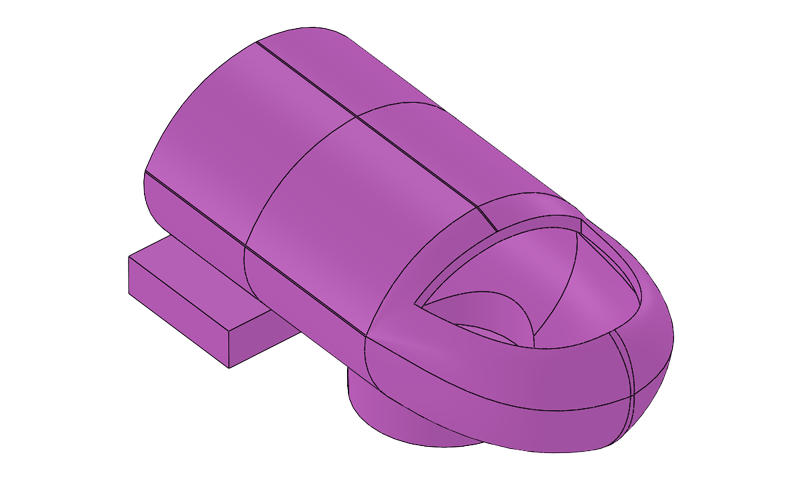
\includegraphics[width=\textwidth]{Chapters/Chapter5/Rigid_Prototypes/Figures/silicon_sleeve_front.png}
        \end{subfigure}
        \begin{subfigure}[b]{0.6\textwidth}
            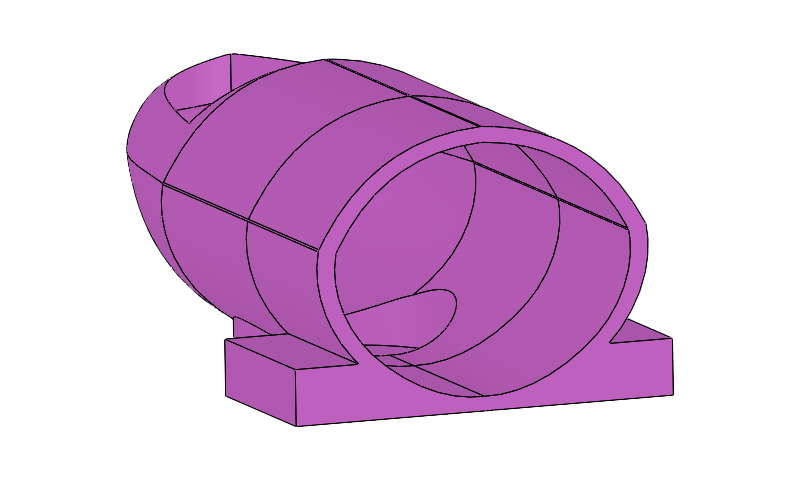
\includegraphics[width=\textwidth]{Chapters/Chapter5/Rigid_Prototypes/Figures/silicon_sleeve_back.png}        
        \end{subfigure}
    }
    \caption{Finger silicon sleeve front and back view}
    \label{fig: finger_sleeve}
\end{figure}

This silicon sleeve was designed to be \textbf{scalable} for different finger sizes and to be easily worn and removed.

\begin{samepage}
    The design is composed of three parts:
    \nopagebreak

    \begin{itemize}
        \item \textbf{Silicon sleeve: } This part was modeled by us on the profile of a real \textbf{3d scanned index finger}, it can be automatically scaled by specifying the index's width as all the measurements are based on that value.
        \item \textbf{Magnet hole: } The hole is designed based on the diameter of the magnet and its height. We also had to find the right \textbf{height tolerance} between the magnet and the pulp to avoid that it could press on the finger too much, impeding vibrations.
        \item \textbf{Mounting wings: } On the sides of the sleeve we have two parallelepipedal wings that are used to \textbf{mount the sleeve} to the structure where the coil will be attached (described in the following section). 
    \end{itemize}
\end{samepage}

Another design problem to solve was the \textbf{positioning} of the magnet, as the design had the goal of being adaptable to different fingertip sizes, we had to consider multiple finger widths. 
For the magnet position we chose the center to be placed on the \textbf{symmetry axis} of the pulp, then we based the design on index fingers with widths between \textbf{13mm} and \textbf{20mm} \cite{index_fingers_width}.
That meant that for 13mm fingers, the magnet size (10mm) was barely smaller than the finger's width, so knowing that the finger tends to get even narrower toward the tip, we had to place the magnet center closer to the \textbf{first interphalangeal fold} rather than to the pulp's center.

\begin{figure}[H]
    \centering
    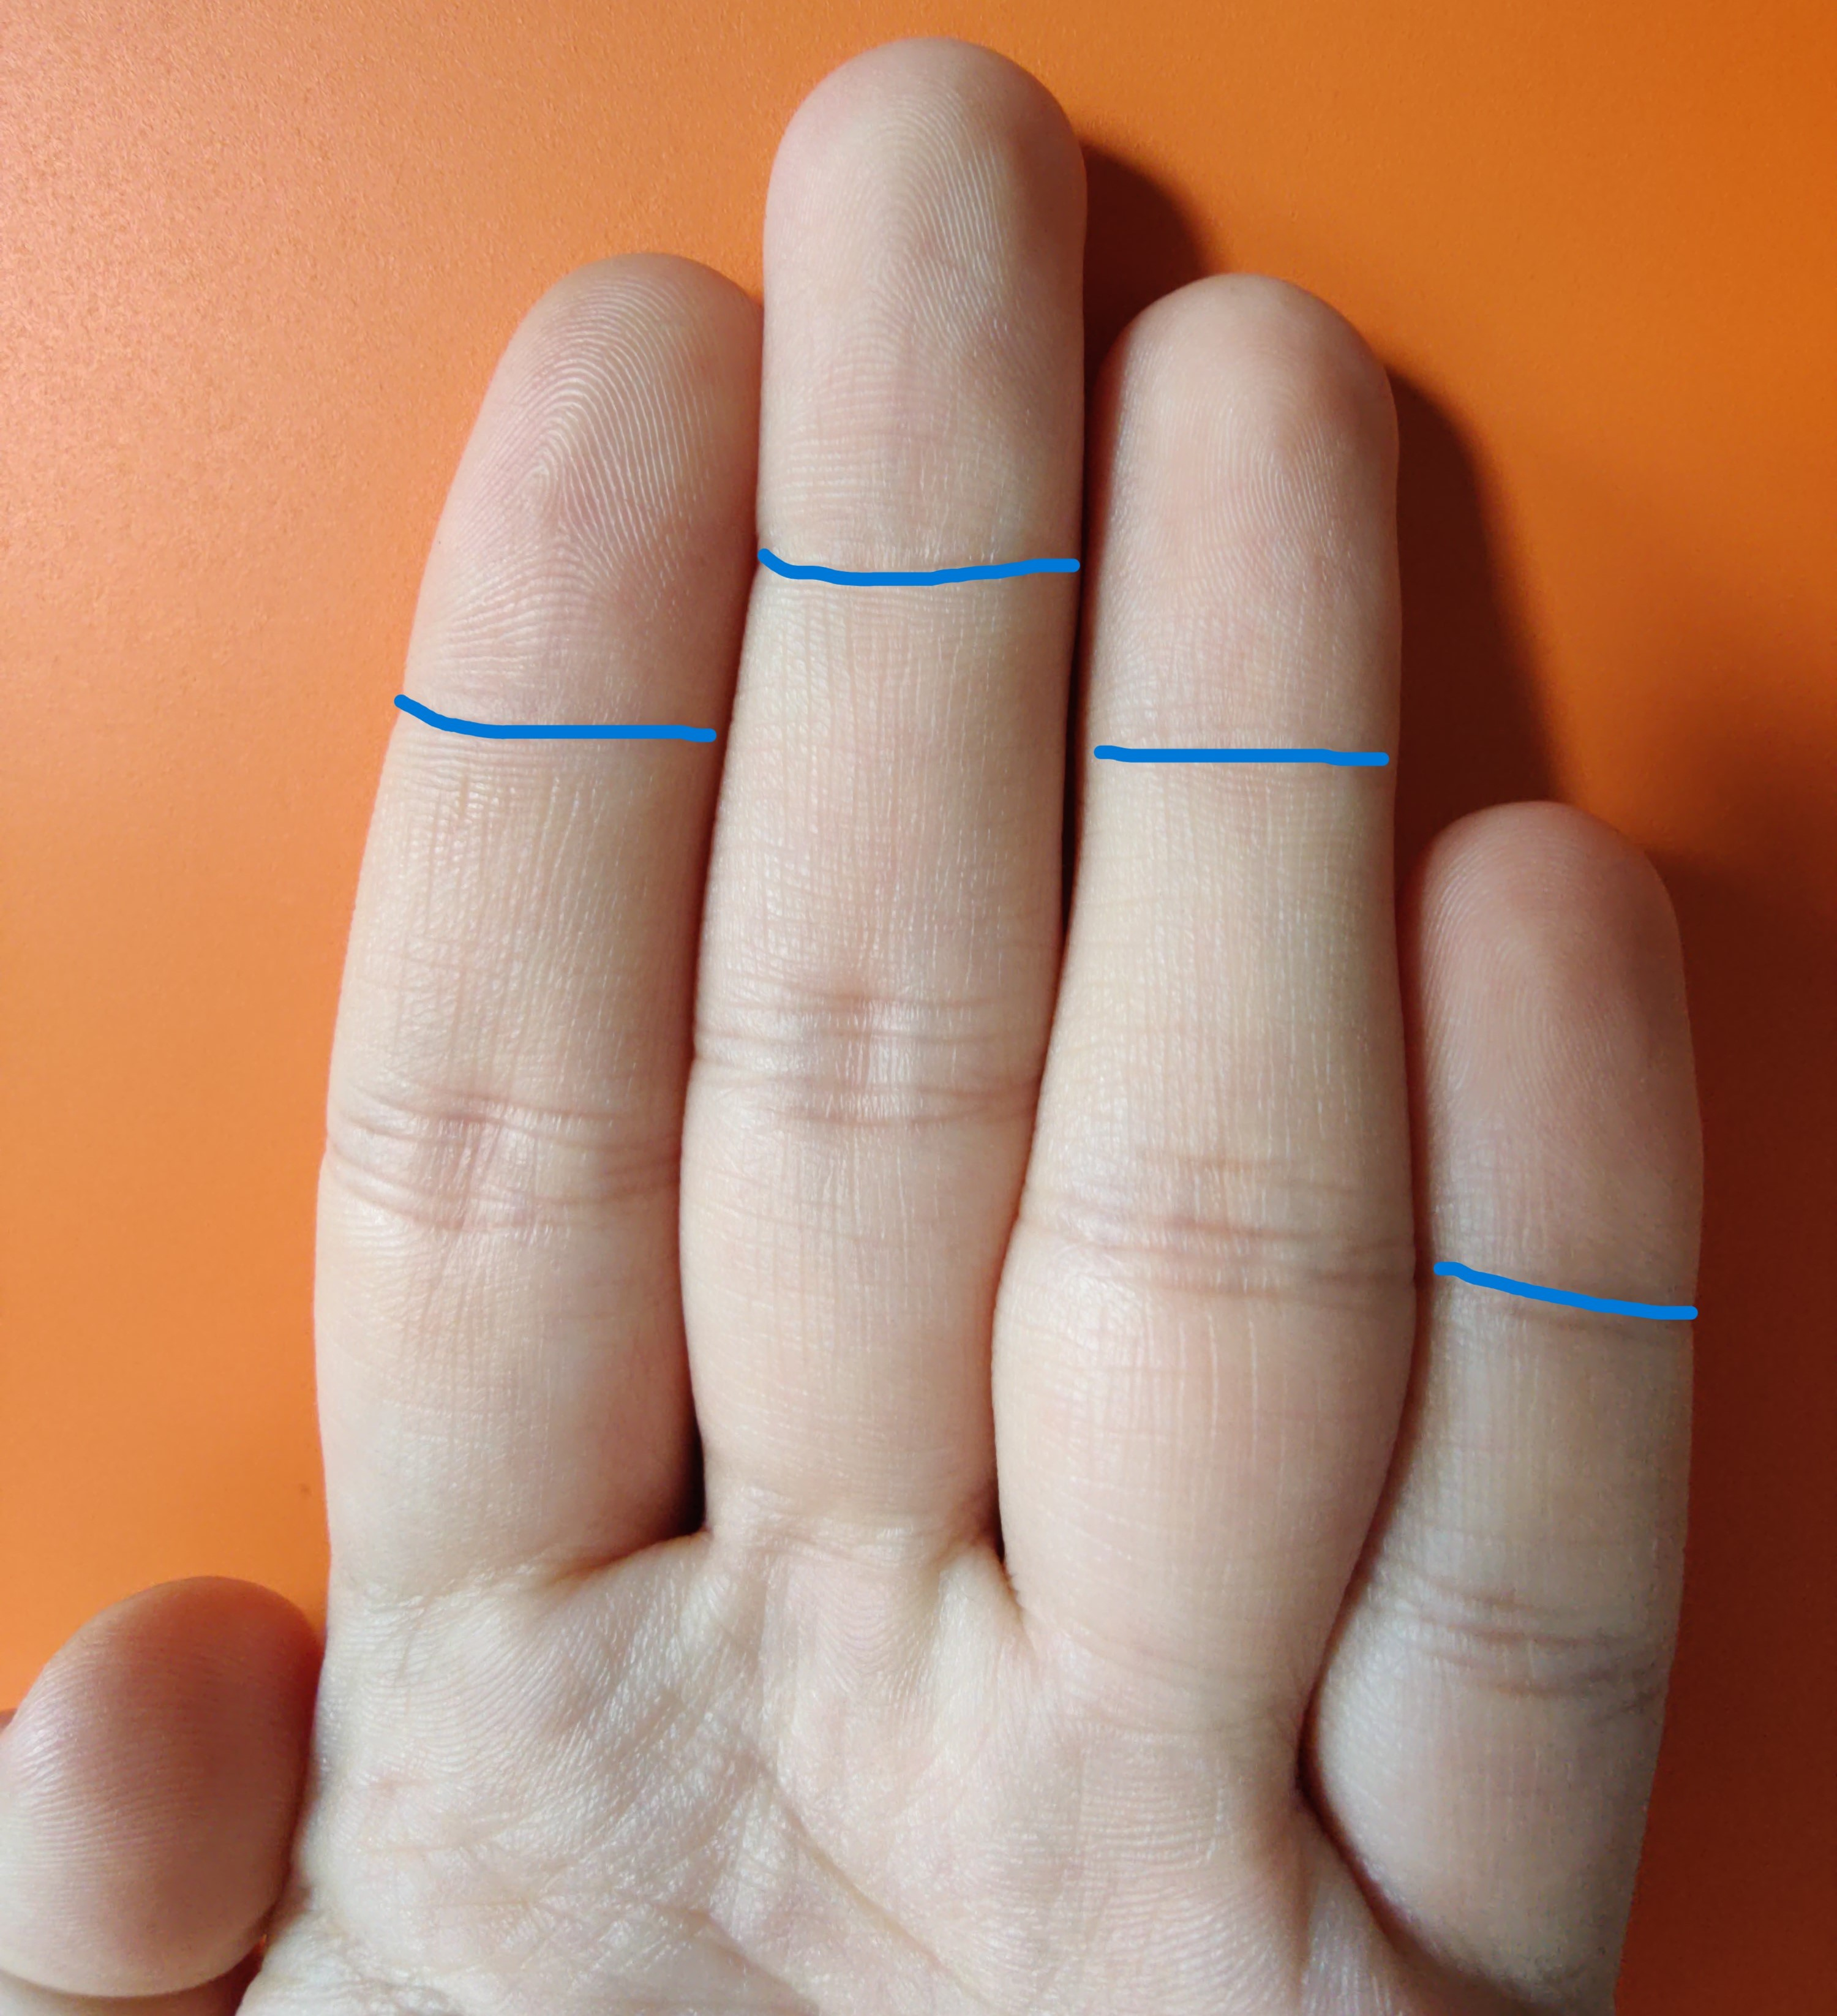
\includegraphics[width=0.4\linewidth]{Chapters/Chapter5/Rigid_Prototypes/Figures/fingers.jpg}
    \caption{In blue we highlighted the first interphalangeal fold for each finger.}
    \label{fig: fingers}
\end{figure}


\subsubsection{Sleeve production}
\label{sec: Sleeve_production}

\begin{samepage}
    The sleeve was produced by \textbf{silicon casting} inside a two-part 3D printed mold:
    \nopagebreak

    \begin{itemize}
        \item \textbf{Mold cavity: } The cavity was designed based on the 3D model of an index finger, with the addition of a small surface to produce an opening at the fingernail (the part in grey in figure \ref{fig: mold_cavity}) and half of the hole necessary to create the magnet cavity.
        \begin{figure}[H]
            \centering
            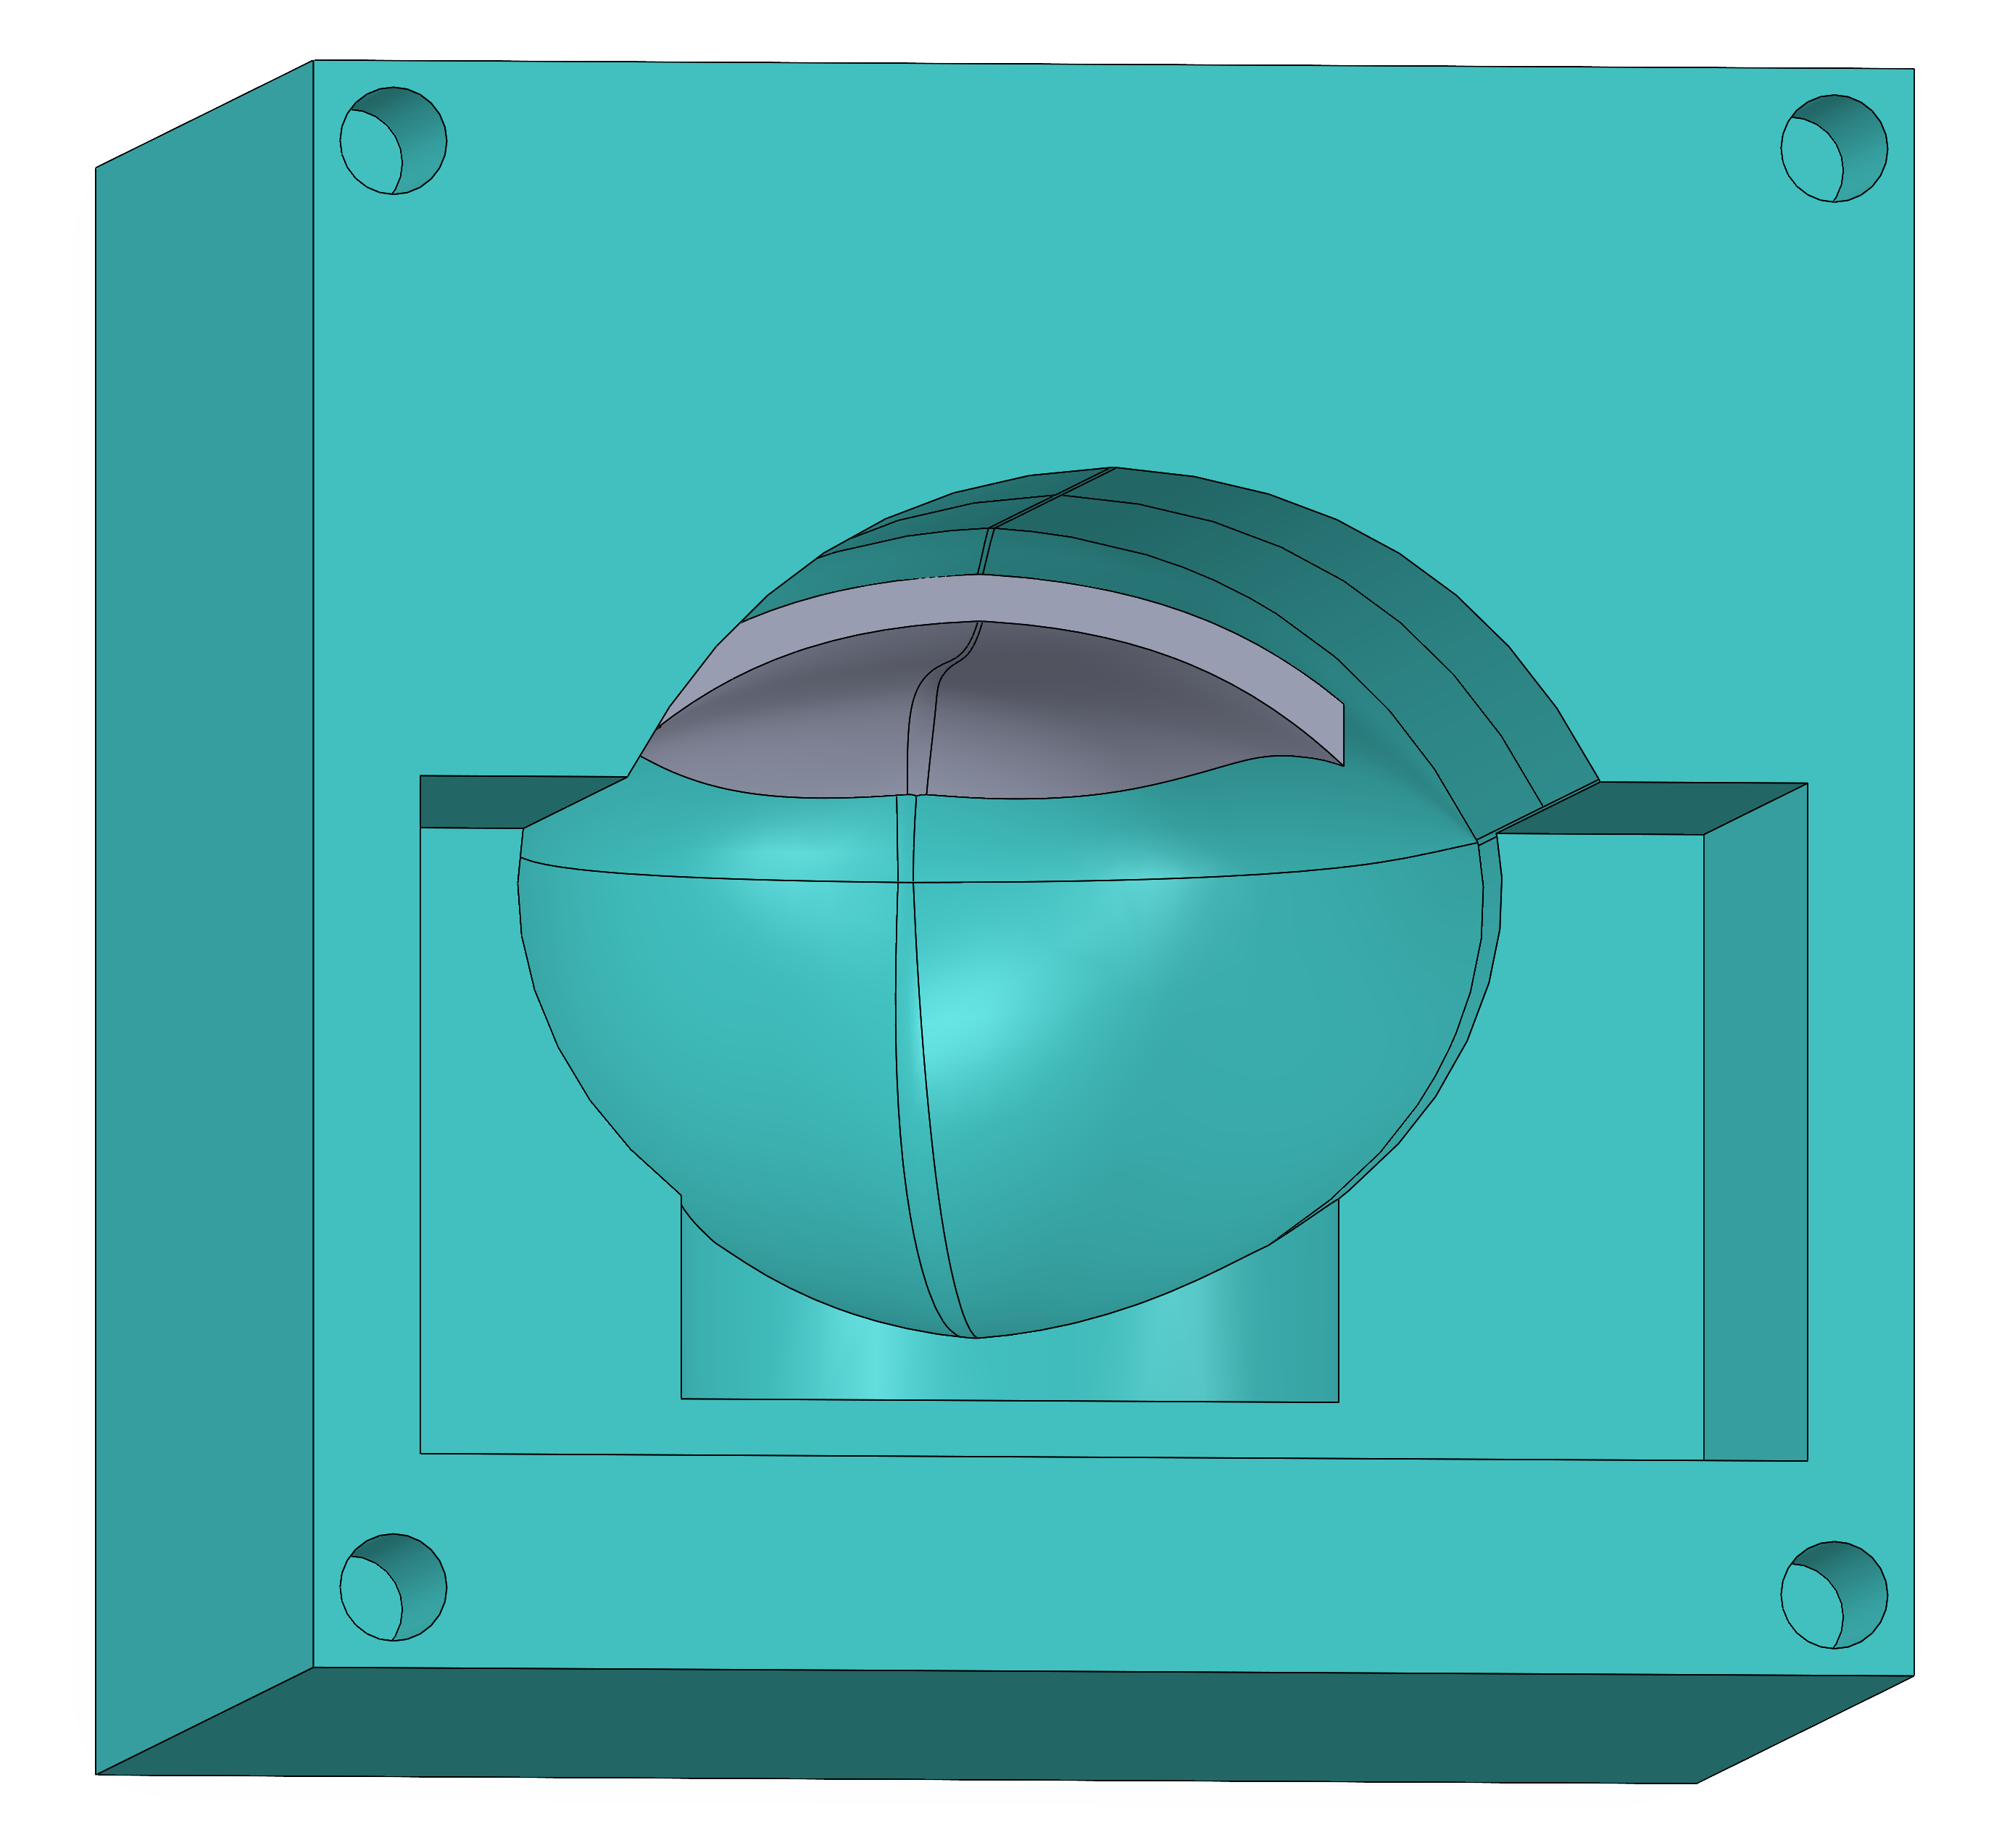
\includegraphics[width=0.4\linewidth]{Chapters/Chapter5/Rigid_Prototypes/Figures/silicon_finger_mold_cavity.PNG}
            \caption{Mold cavity}
            \label{fig: mold_cavity}
        \end{figure}

        \item \textbf{Mold core: } The core was designed to be the negative of the cavity, including a part to create the other half of the magnet cavity and mounting wings (the part in light blue in figure \ref{fig: mold_core}).
        The negative is scaled down a bit to create a \textbf{casting clearance} of about \textbf{0.8mm}.
        This part also includes a cap that is screwed on the cavity to keep the core \textbf{suspended} in the silicon.
        \begin{figure}[H]
            \centering
            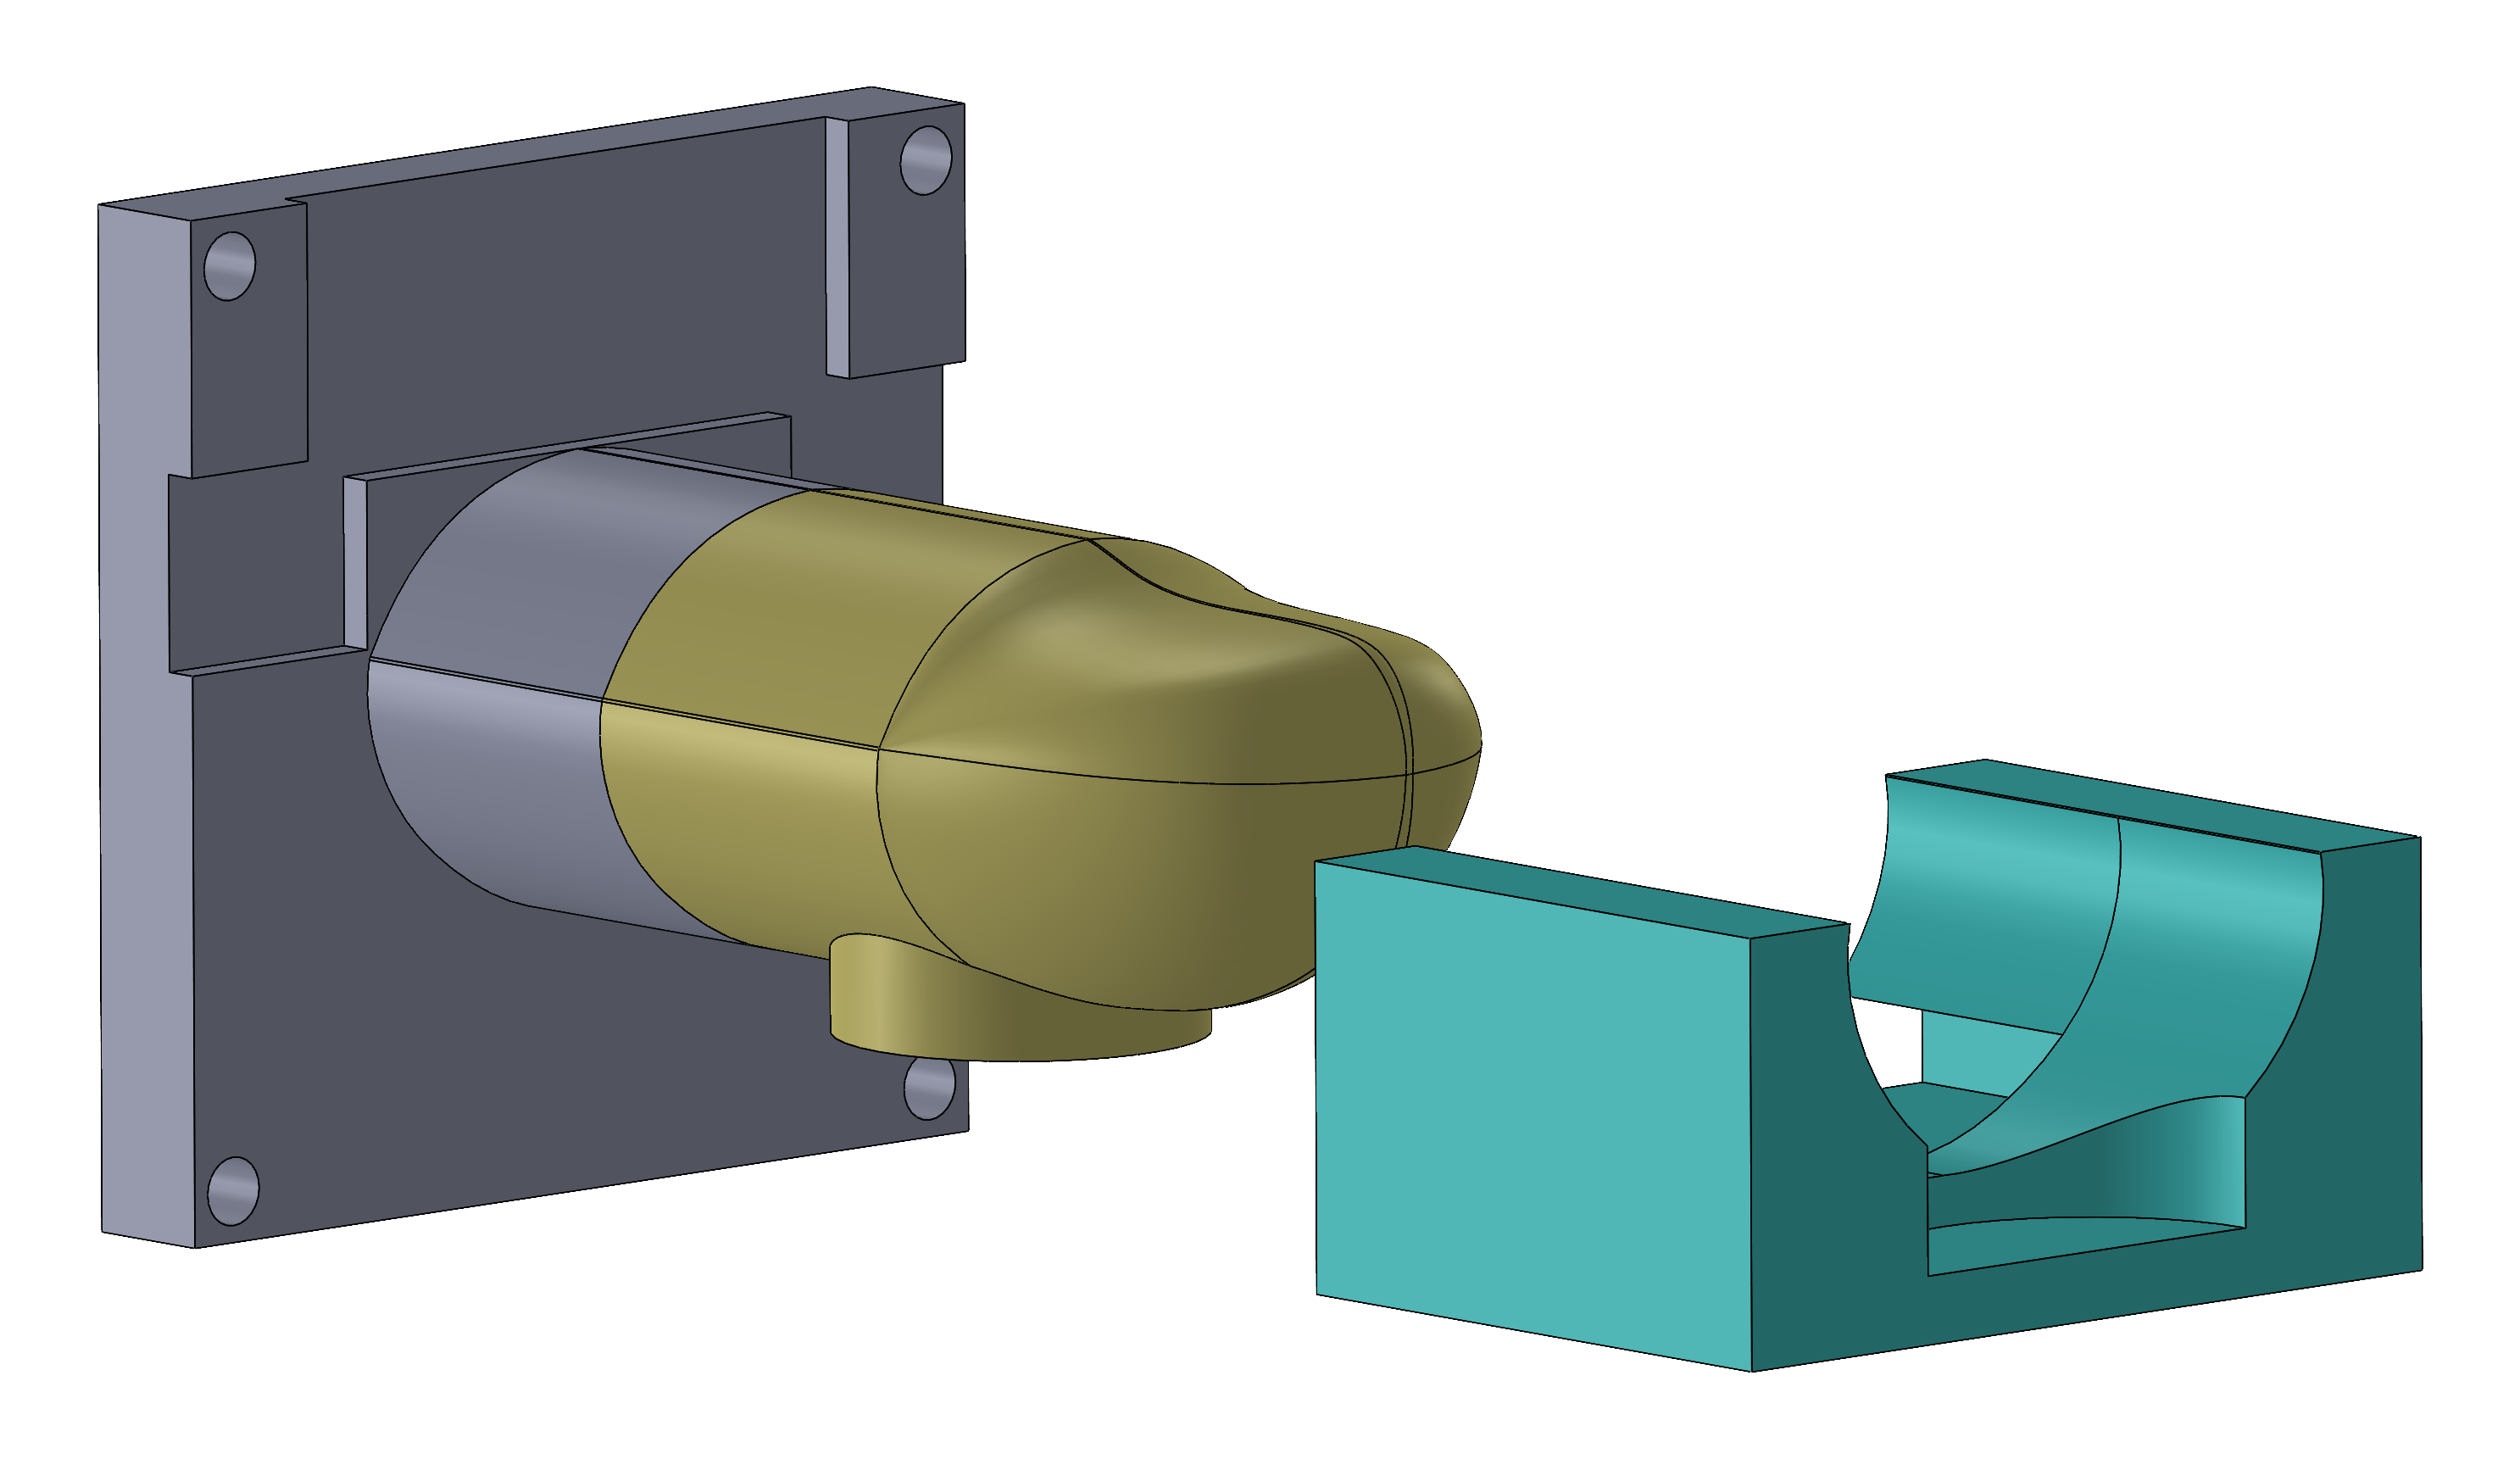
\includegraphics[width=0.5\linewidth]{Chapters/Chapter5/Rigid_Prototypes/Figures/silicon_finger_mold_core.PNG}
            \caption{Exploded view of the mold core}
            \label{fig: mold_core}
        \end{figure}
    \end{itemize}
\end{samepage}


The part went through multiple iterations to land on the \textbf{right thicknesses for the sleeve itself}, it needed to be thin enough to be \textbf{adaptable} to multiple fingers (considering similar widths) but not so thin as to be \textbf{durable} enough.

The material used for the casting was a \textbf{two-component silicon rubber} from ResChimica.
We tested two different types of silicon, one with a \textbf{shore hardness} of \textbf{12} \cite{R_Pro_10_silicon} and one with a shore hardness of \textbf{35} \cite{R_Pro_Fast_silicon}.

From our tests, we found that the silicon with a shore hardness of \textbf{35} was \textbf{too rigid} and \textbf{absorbed too much vibration} so we decided to use the softer one.
The only problem with this softer silicon was its minimum curing time of \textbf{3 hours} at room temperature which always had to be increased as it never cured completely in that time.

\subsubsection{Magnet-coil distancing structure}
We then focused on a structure able to keep the coil at a \textbf{fixed distance} from the silicon sleeve and magnet.
The design goals for this device were that it should be lightweight, easily wearable and adaptable to multiple sleeves' sizes.

% \begin{figure}[H]
%     \centering
%     \begin{subfigure}[b]{0.475\textwidth}
%         \centering
%         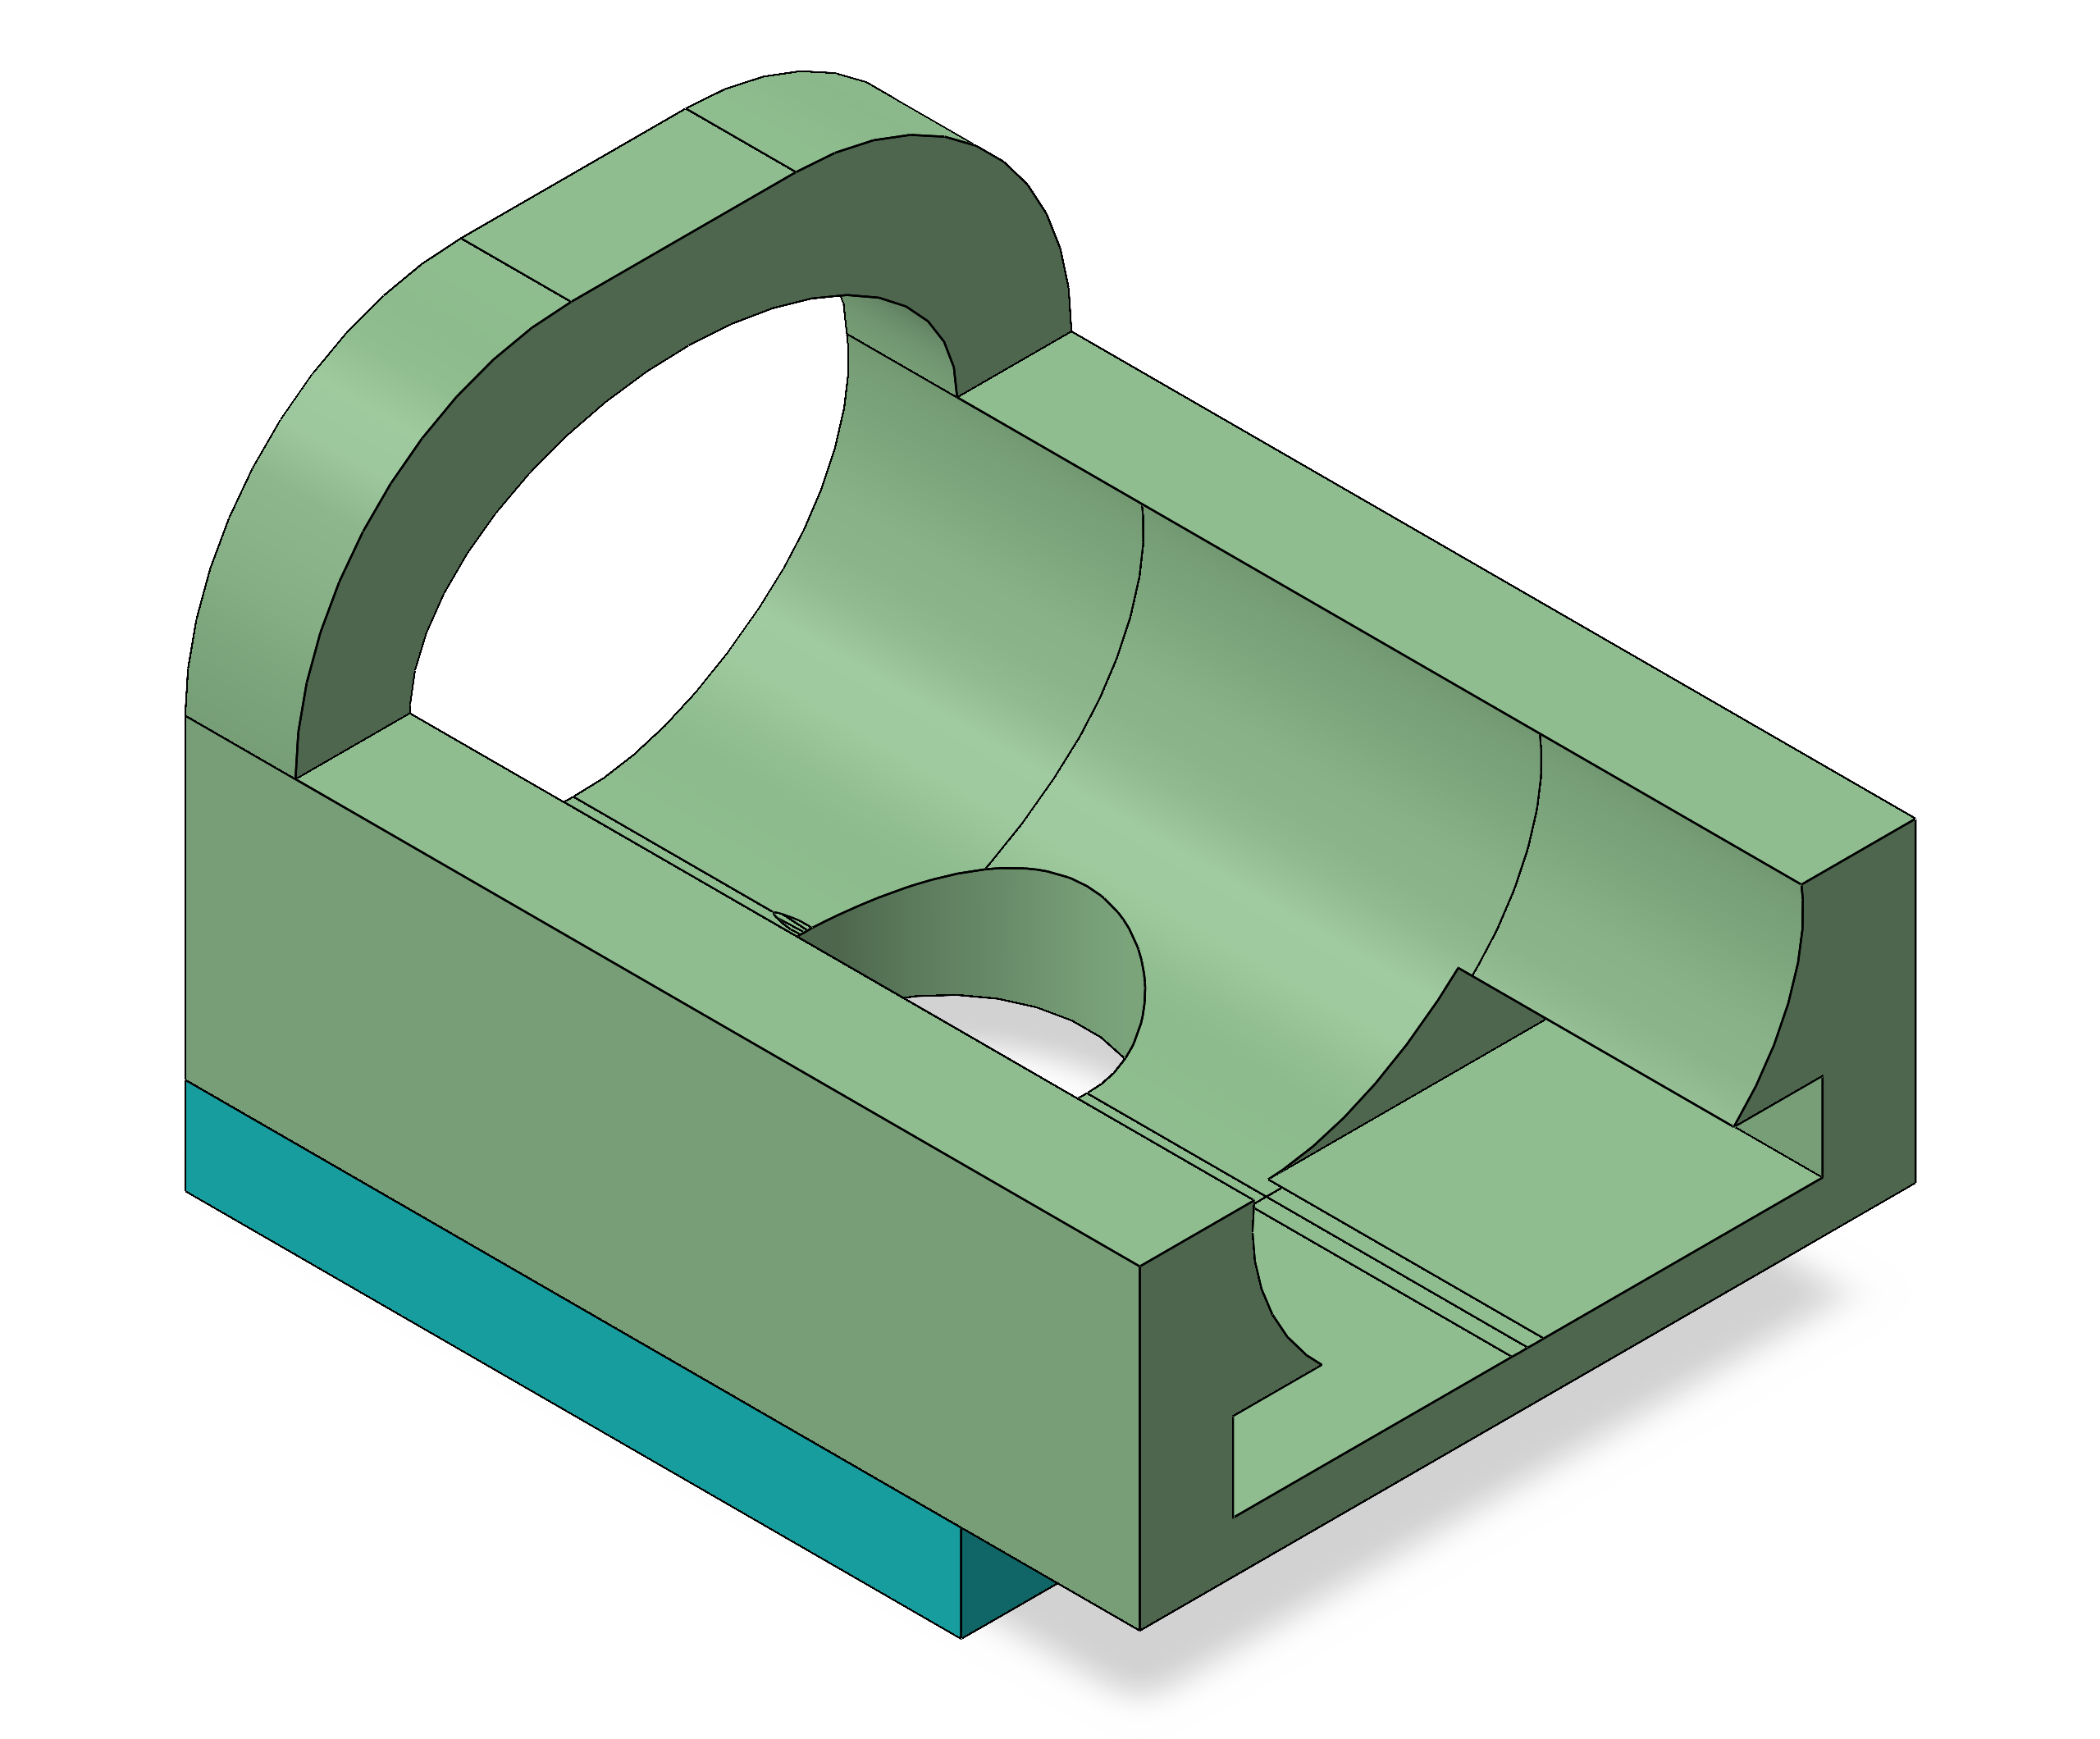
\includegraphics{Chapters/Chapter5/Flexible_Mat_Prototypes/Figures/sleeve_holder_top.PNG}
%         \caption{Sleeve holder top view.}
%         \label{fig: sleeve_holder_top}
%     \end{subfigure}
%     \hfill
%     \begin{subfigure}[b]{0.475\textwidth}
%         \centering
%         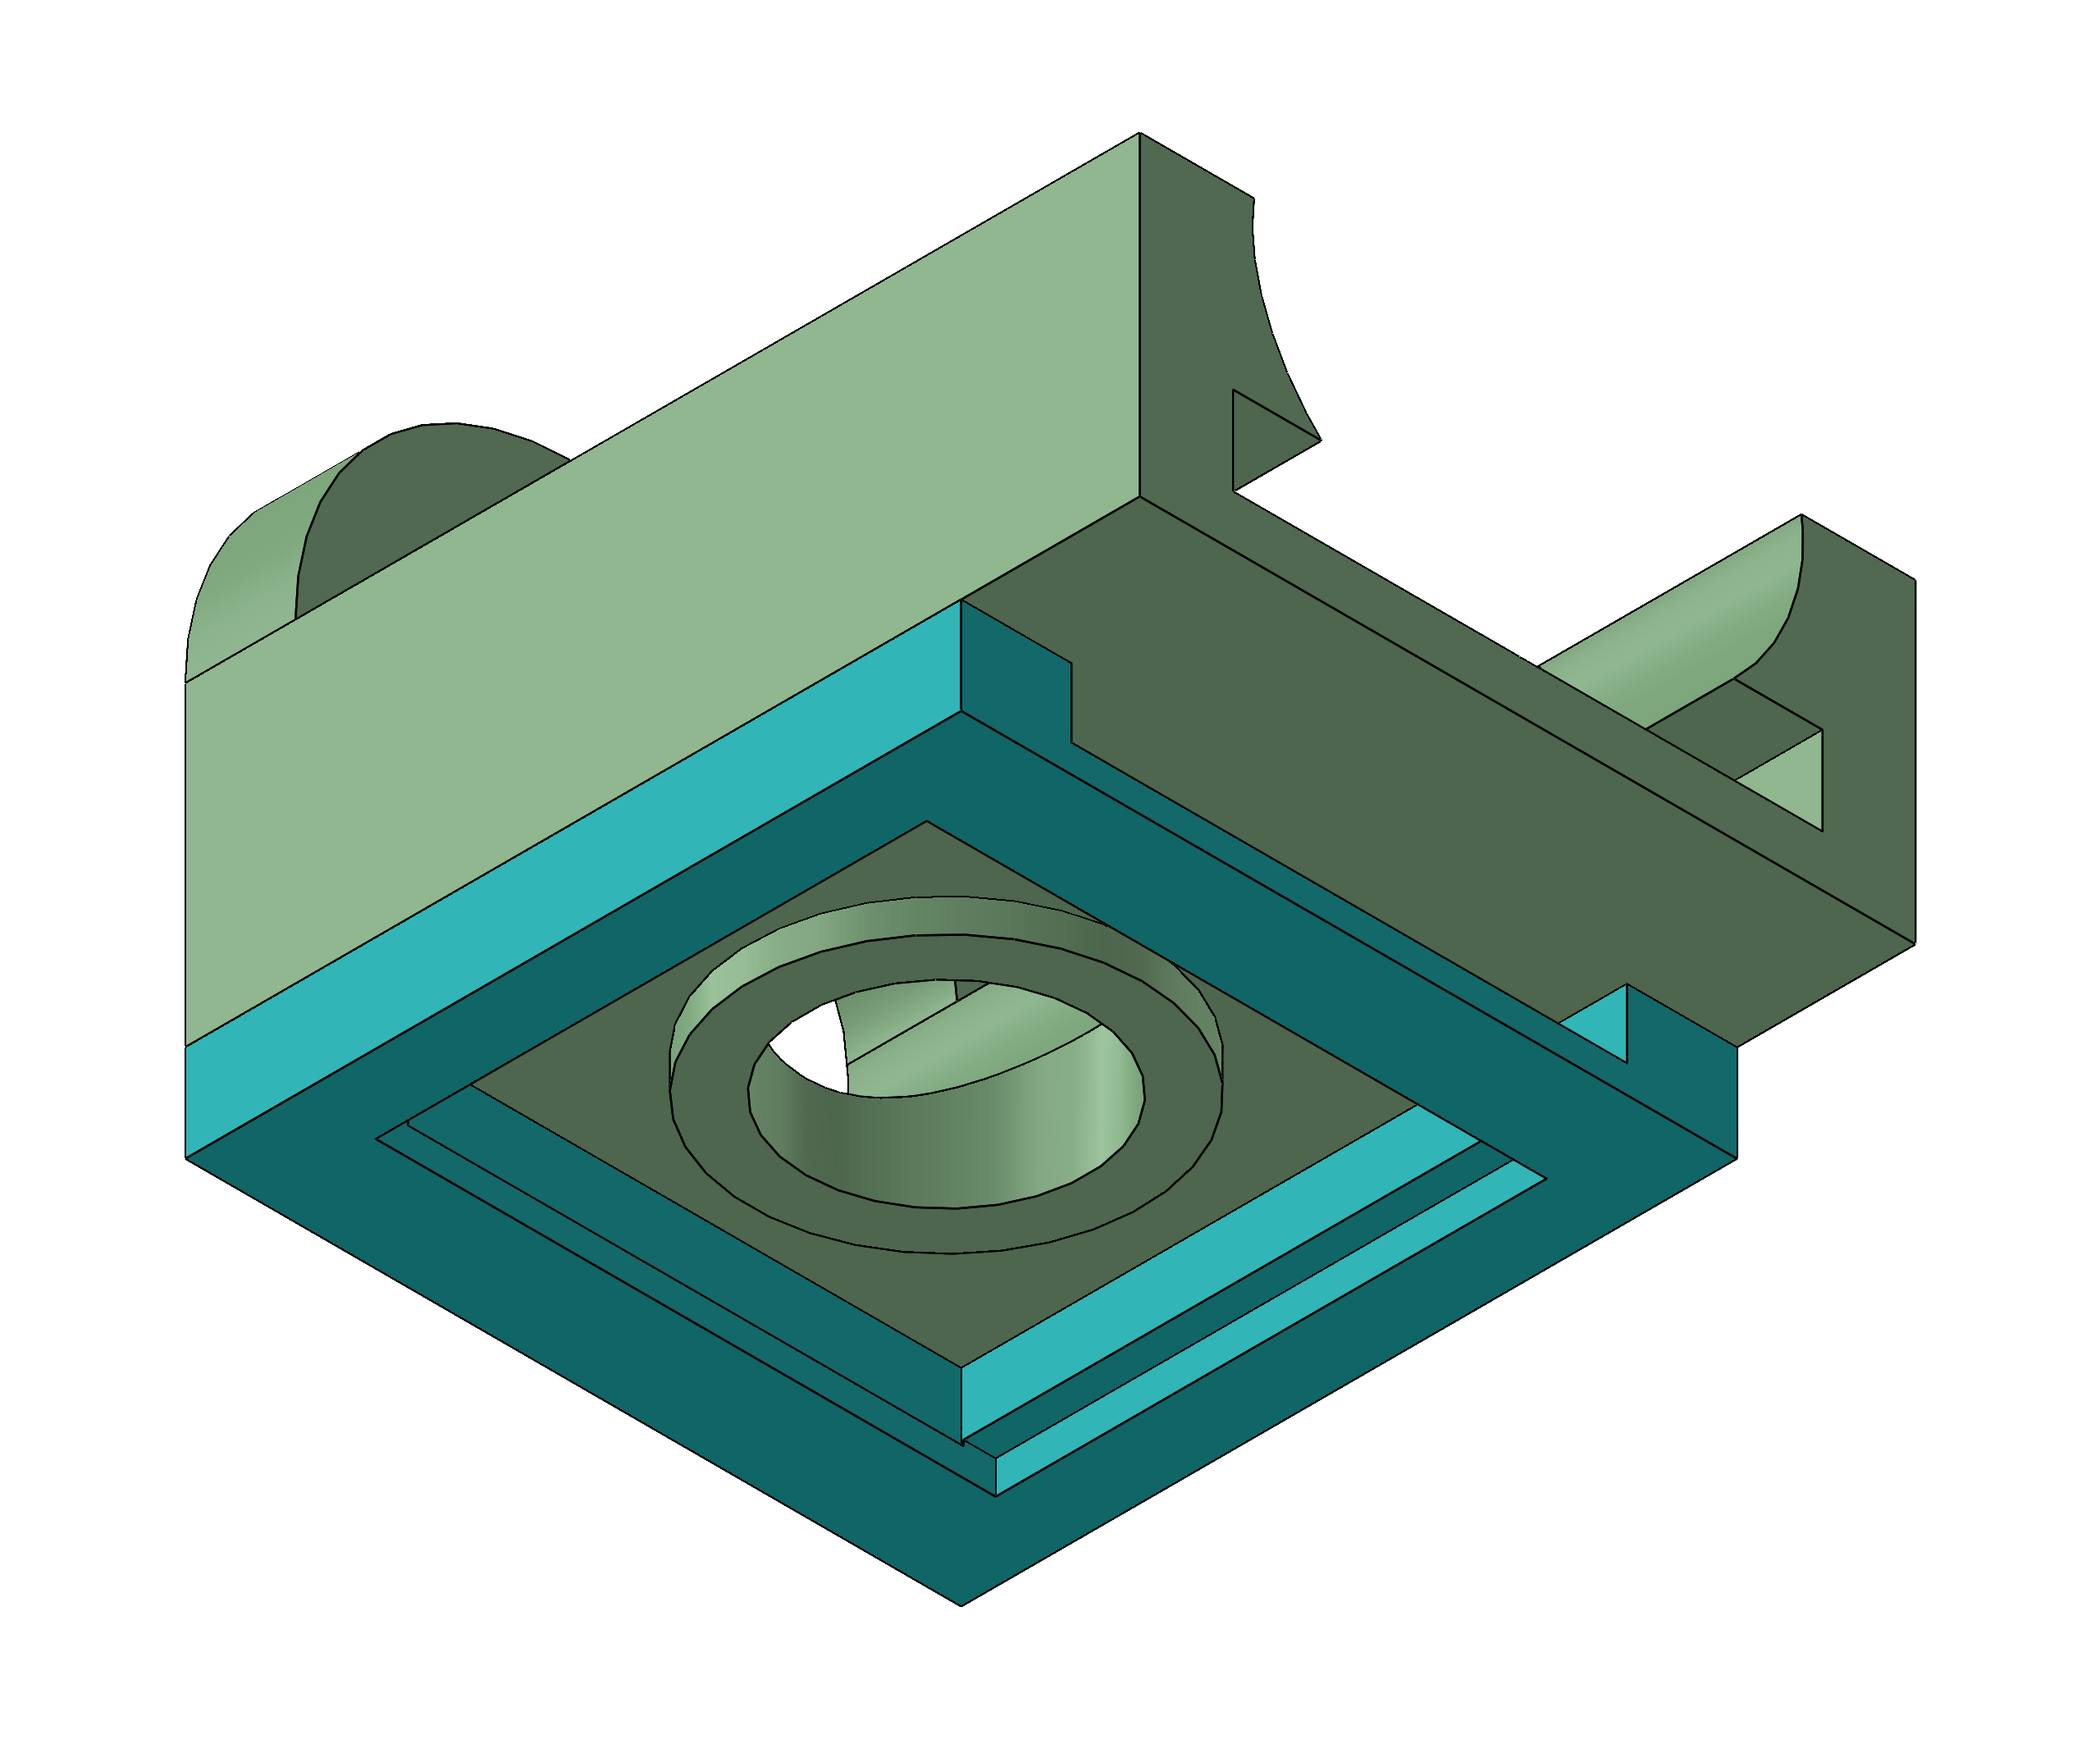
\includegraphics{Chapters/Chapter5/Flexible_Mat_Prototypes/Figures/sleeve_holder_btm.PNG}
%         \caption{Sleeve holder bottom view.}
%         \label{fig: sleeve_holder_btm}
%     \end{subfigure}
%     \caption{Silicon sleeve holder}
%     \label{fig: sleeve_holder}
% \end{figure}

After multiple iterations, we landed on a three-component design.
\begin{itemize}
    \begin{samepage}
        \item \textbf{Sleeve holder: } This component (represented in Fig. \ref{fig: sleeve_holder}) is the structure where the sleeve can be attached, this is done by inserting the mounting wings inside the two squared holes on the bottom of the part.
        The circle hole at the center of the component is where the magnet cavity of the sleeve with the magnet inside will be placed.
        The arch on the component front is present to allow the tip of the finger to support the weight of the structure.
        \nopagebreak

        \begin{figure}[H]
            \centering
            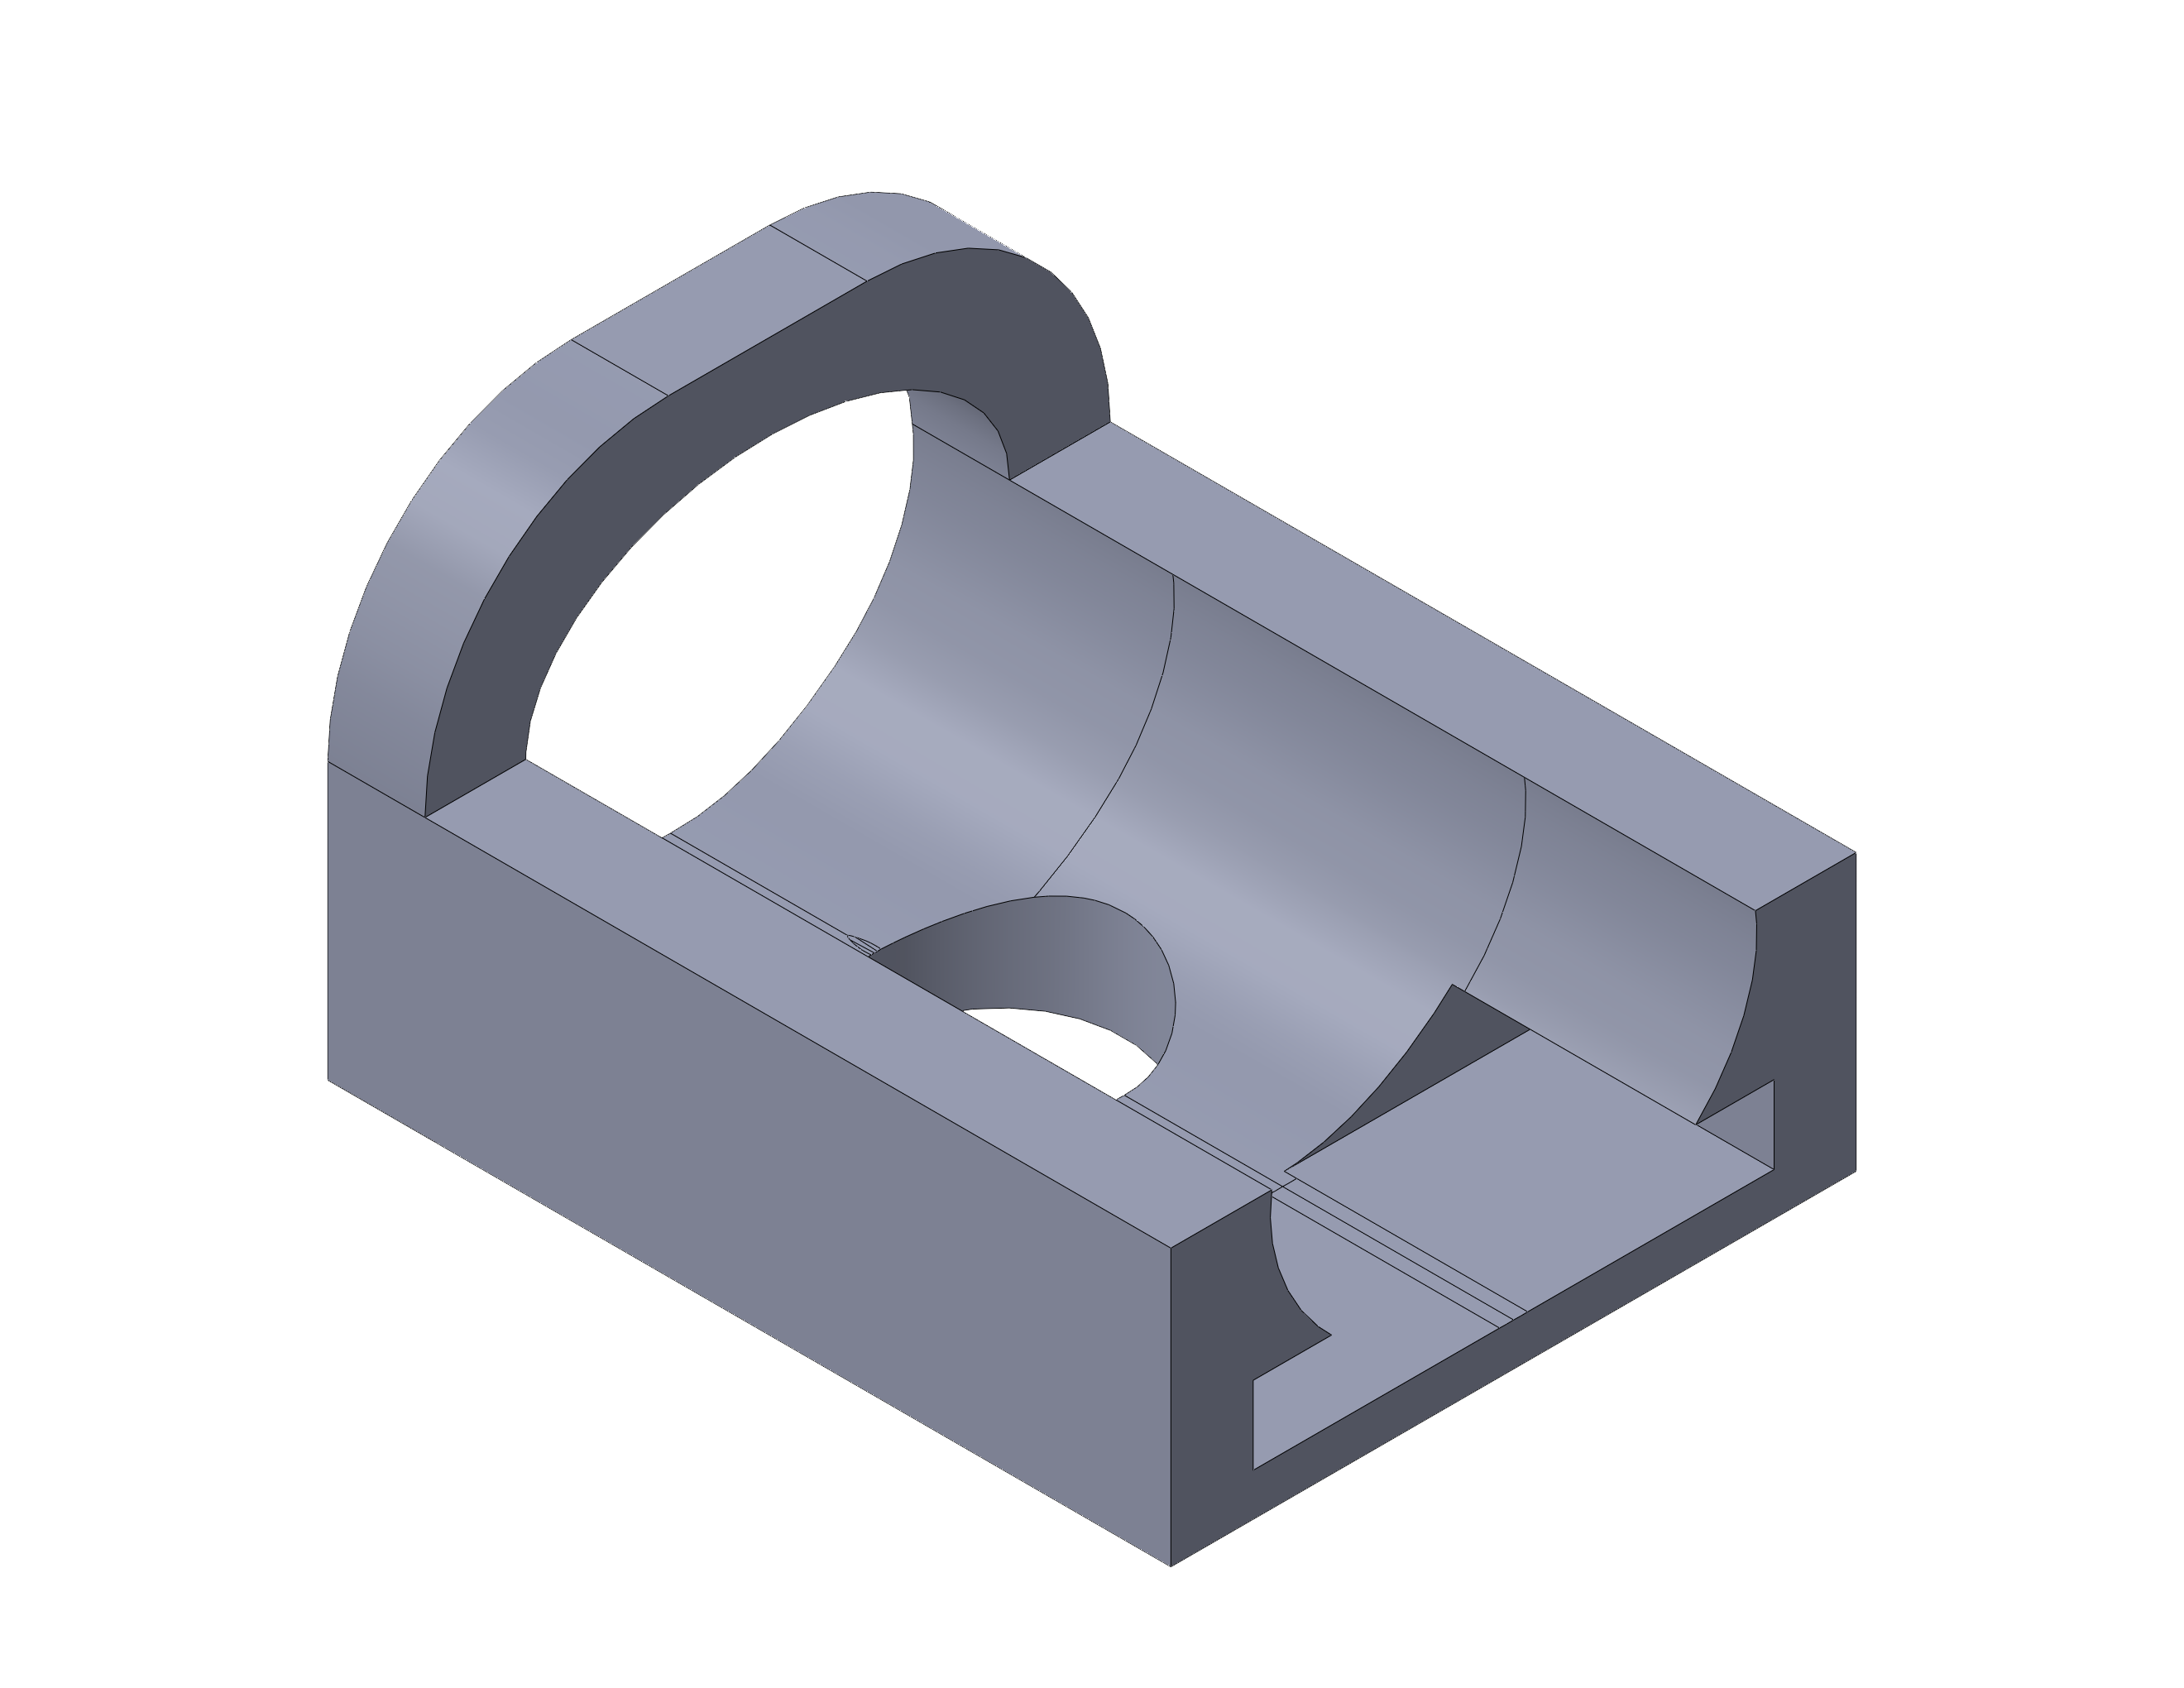
\includegraphics[width=0.5\linewidth]{Chapters/Chapter5/Rigid_Prototypes/Figures/sleeve_holder.png}
            \caption{Silicon finger sleeve holder}
            \label{fig: sleeve_holder}
        \end{figure}
    \end{samepage}
    
    \begin{samepage}
        \item \textbf{Coil trap: } This component is the structure where the coil is inserted. This component is composed of 3 parts, a heatsink, a coil holder and a mask to screw the heatsink to the sleeve holder.
        The coil is sandwiched between the heatsink (the part in bronze in Fig. \ref{fig: coil_trap}) and the coil holder (the part in grey in Fig. \ref{fig: coil_trap}). 
        \nopagebreak

        Then they are screwed together to the sleeve holder.
        \nopagebreak

        \begin{figure}[H]
            \centering
            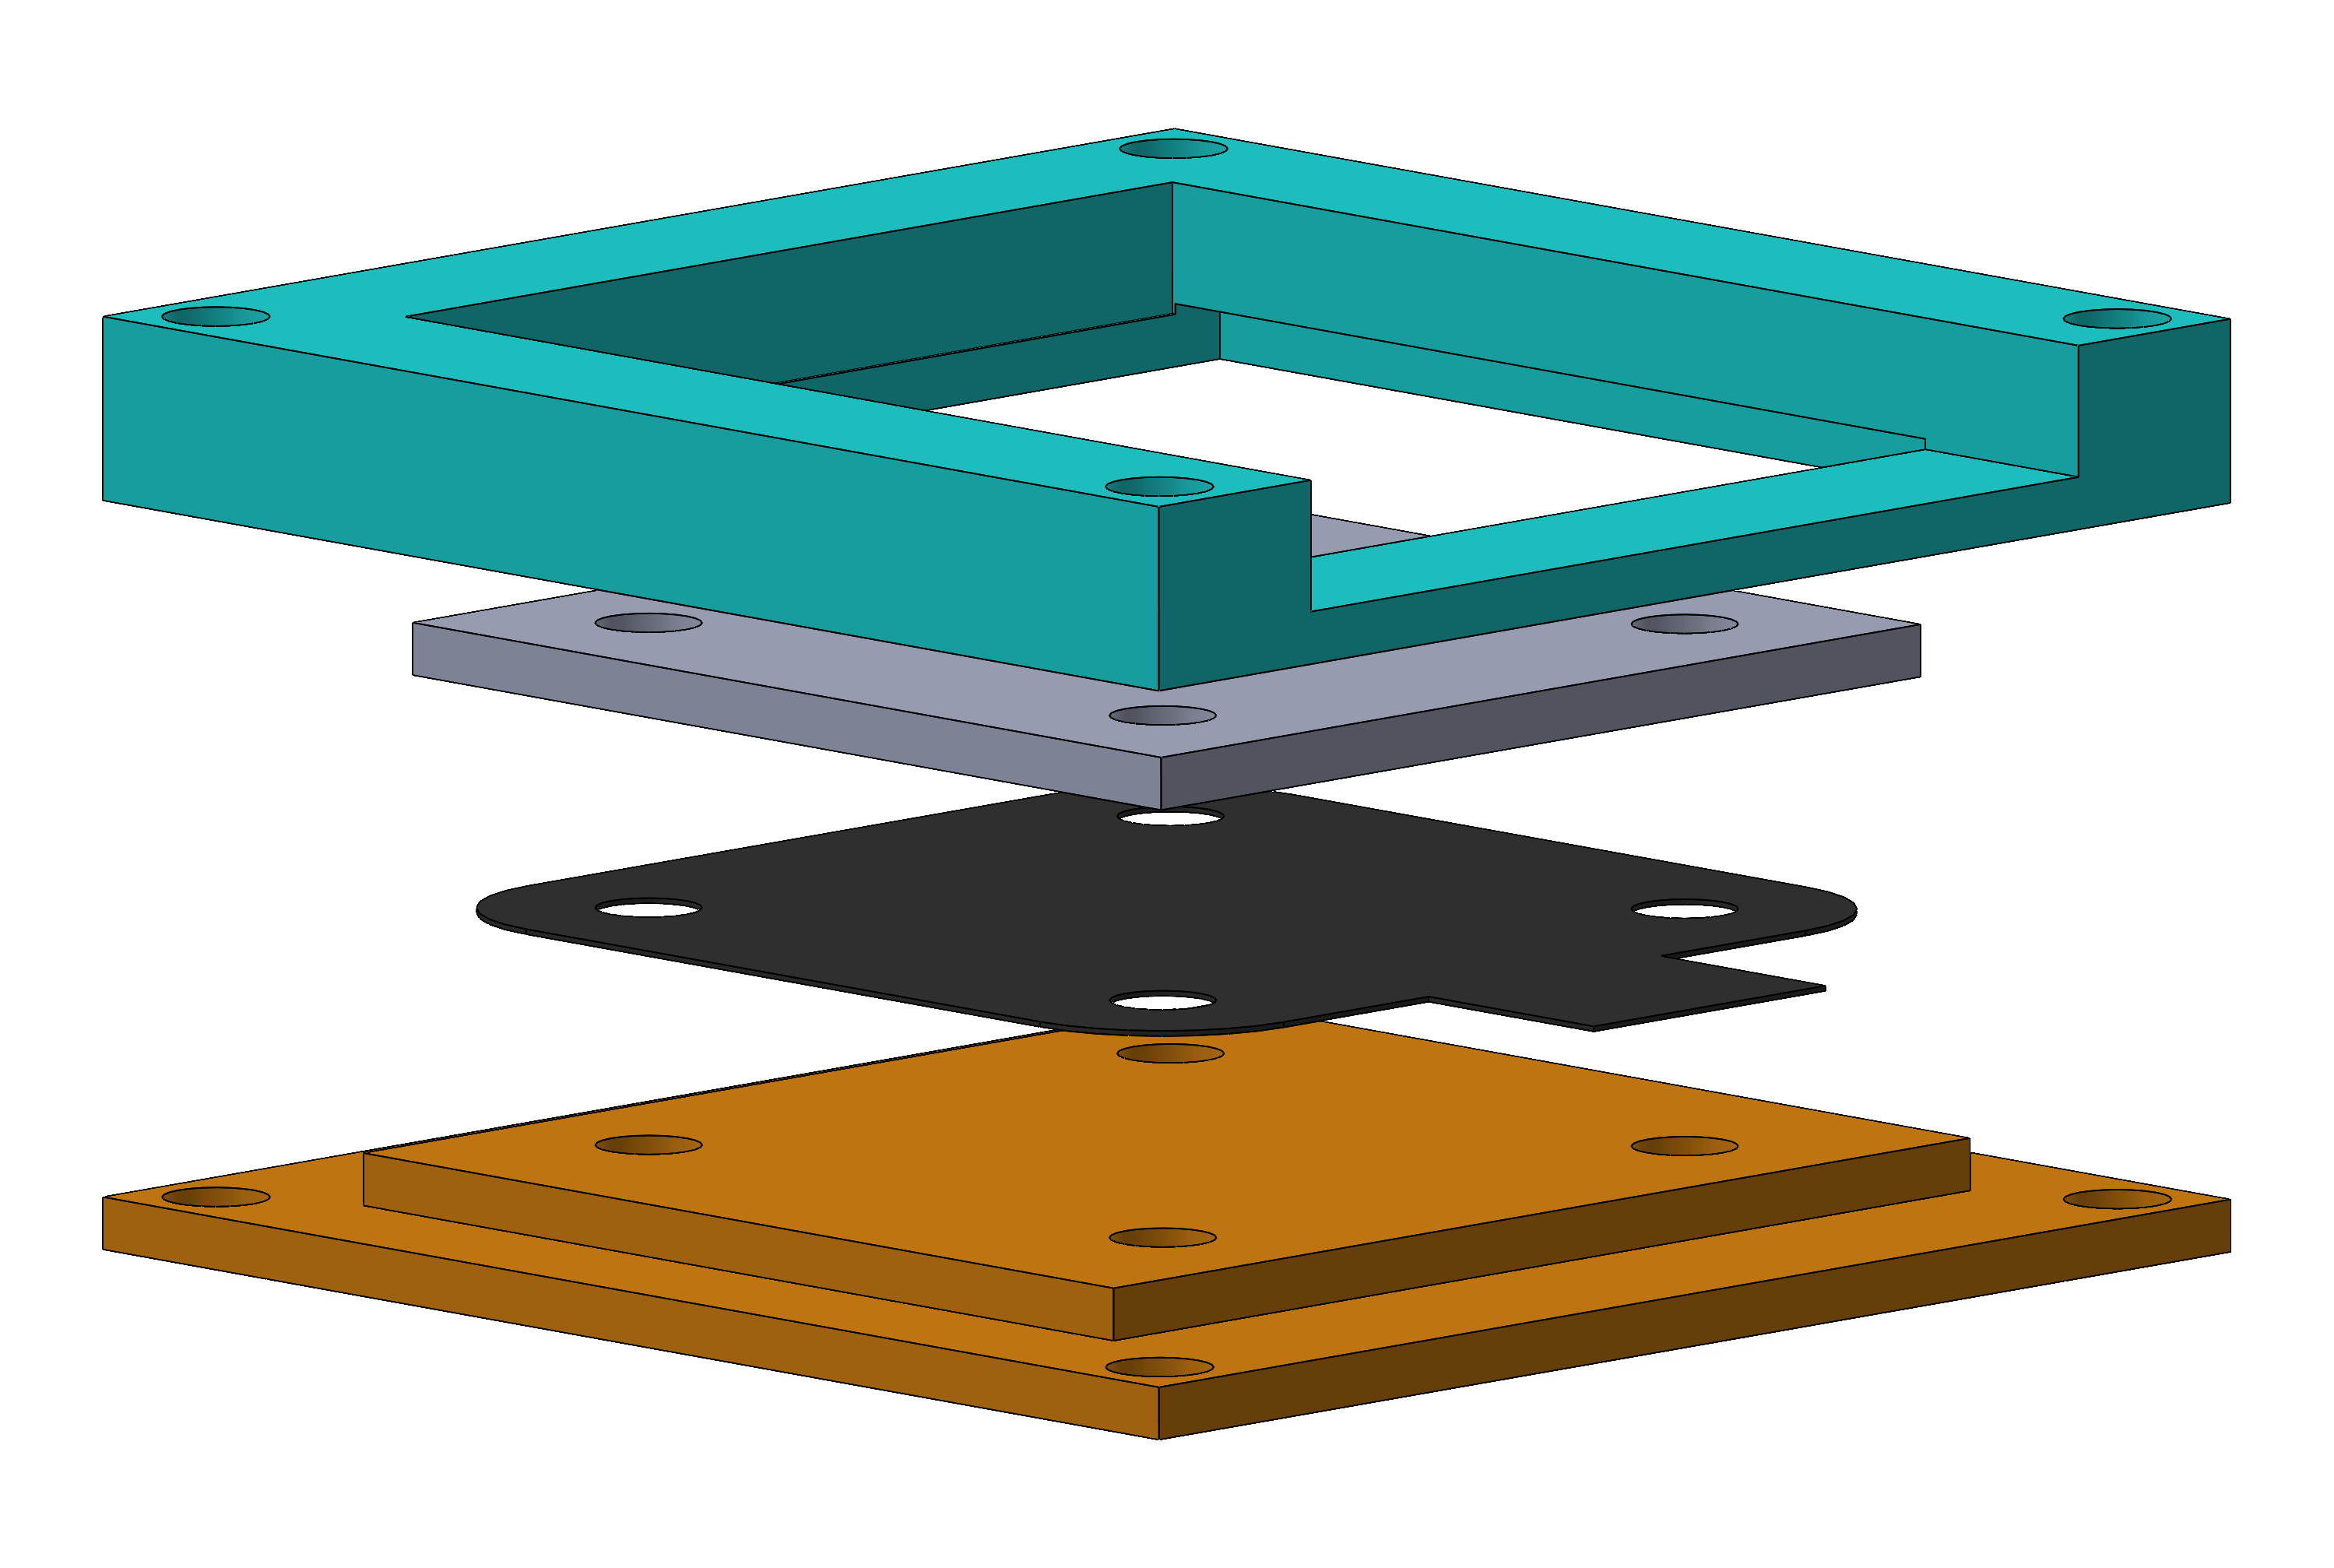
\includegraphics[width=0.5\linewidth]{Chapters/Chapter5/Rigid_Prototypes/Figures/coil_trap.png}
            \caption{Explode of the coil trap}
            \label{fig: coil_trap}
        \end{figure}
    \end{samepage}
    
\end{itemize}

\subsubsection{Heat dissipation}
As the coil while active produces a lot of \textbf{heat}, we decided to introduce a \textbf{heatsink} in the design (the part in bronze in figure \ref{fig: coil_trap}).
The heatsink was made by cutting two small strips from a thin sheet of \textbf{copper} (\textbf{1mm} thick) that are joined together by \textbf{thermal paste} and screws.
The same screws are also used to keep in place the coil and the coil holder.

For the same heat dissipation reason, we printed all components in \textbf{ABS} as it has a higher melting point than PLA.

\subsubsection{Prototype usability}
This prototype was much more usable than the previous one.
The magnet was also kept at the right distance from the coil and the vibrations were \textbf{much more noticeable}, also being \textbf{wearable} made it much easier to use.
The biggest problem of this prototype was the silicon sleeve, as the silicon tends to \textbf{absorb} some of the vibrations produced by the coil and the softness of the material made the \textbf{mounting mechanism} a bit \textbf{unreliable}.
We also had to add a small \textbf{blowing fan} and another part to the heatsink (as we can see in figure \ref{fig: rigid_prot}) to keep the coil cool as it would \textbf{heat a lot} after a few minutes of use.

\begin{figure}[H]
    \centering
    \resizebox{1\textwidth}{!}{
        \begin{subfigure}[b]{0.45\textwidth}
            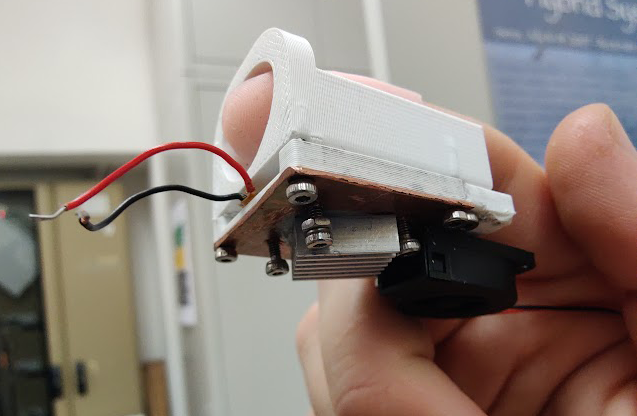
\includegraphics[width=\textwidth]{Chapters/Chapter5/Rigid_Prototypes/Figures/rigid_prot_btm.png}
        \end{subfigure}
        \begin{subfigure}[b]{0.45\textwidth}
            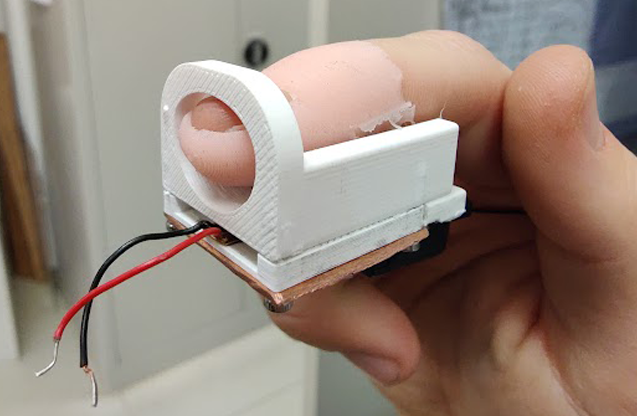
\includegraphics[width=\textwidth]{Chapters/Chapter5/Rigid_Prototypes/Figures/rigid_prot_top.png}        
        \end{subfigure}
    }
    \caption{Bottom and top view of the real prototype}
    \label{fig: rigid_prot}
\end{figure}



%----------------------------------------------------------------------------------------
%	SECTION 2
%----------------------------------------------------------------------------------------
\section{Flexible Mat Prototypes}
%\label{sec:Flexible_Mat_Prototypes}

% -- Subsection 3.1
\subsection{Design of the membrane}

\subsubsection{Material stiffness and thickness}

\subsubsection{Membrane structure vs magnet dimensions}


% -- Subsection 3.2
\subsection{Design of the mat}

\subsubsection{Distance magnet-coil}

\subsubsection{Coil trap}

\subsubsection{Production method and structure}


% -- Subsection 3.3
\subsection{Design faults and problems}

\subsubsection{Membrane fragility}

\subsubsection{Overall system flexibility}

\subsubsection{Keeping the distance coil-magnet under finger pressure}

\subsubsection{Production method}

%----------------------------------------------------------------------------------------
%	SECTION 2
%----------------------------------------------------------------------------------------
\section{Experimentation and Evaluation}
In this section, we will present the results of the experiments we conducted on the coil itself and the flexible mat prototypes.
We will start by presenting the results of the heating tests we conducted on the coil.
Then we will move on to the results of the force response tests we conducted on the flexible mat prototypes.

% -- Subsection 3.1 
\subsection{Heating testing}
As we discussed in previous sections coils have a critical issue with heating.
This is because the coil is a resistive element that generates heat when current flows through it.
This is the main reason why the coil cannot produce very high magnetic fields and in turn high magnetic repulsion forces.
With these tests, we wanted to understand the limits of Flexar coils, in this way, we wanted to reach an optimal working point and configuration for our prototypes.
The configurations we tested were two, one considering only one coil and the other considering two coils connected in parallel.
Both were then tested in DC and AC conditions.

For the DC test, the coils were connected to an RND 320-KA300SP bench power supply with which we did a voltage sweep from 0.5V to 4V, with 0.5V steps.

Meanwhile, for the AC test, we used an Agilent 33220A function generator and a Kepco BOP 20-10M bipolar power amplifier.
The power amplifier was set to amplify the input signal with a voltage gain of 10. 
Two types of AC tests were conducted, both were done with sine waves at 200Hz.
In the first type, the function generator was set to output a bipolar sine wave from -$V_{max}$ to $V_{max}$, with $V_{max}$ being the voltage we wanted to test.
In the second type, the function generator was set to output a unipolar sine wave from 0 to $V_{max}$.
Then we devised a voltage [0.5, 6]V ([0.05, 0.6] on the signal generator), 0.5V steps for the $V_{max}$ sweep.
The voltage limits we chose were based on the maximum voltage the coil could withstand before reaching its thermal runaway point.

To measure the temperature of the coil we used a multimeter connected to a thermocouple.
The coil/s were placed on a piece of wood to avoid heat dissipation through the table, and the thermocouple was placed on top of the coil/s.
To keep both in place they were taped to the wood with electrical tape.
\begin{figure}
    \centering
    \resizebox{0.9\textwidth}{!}{
        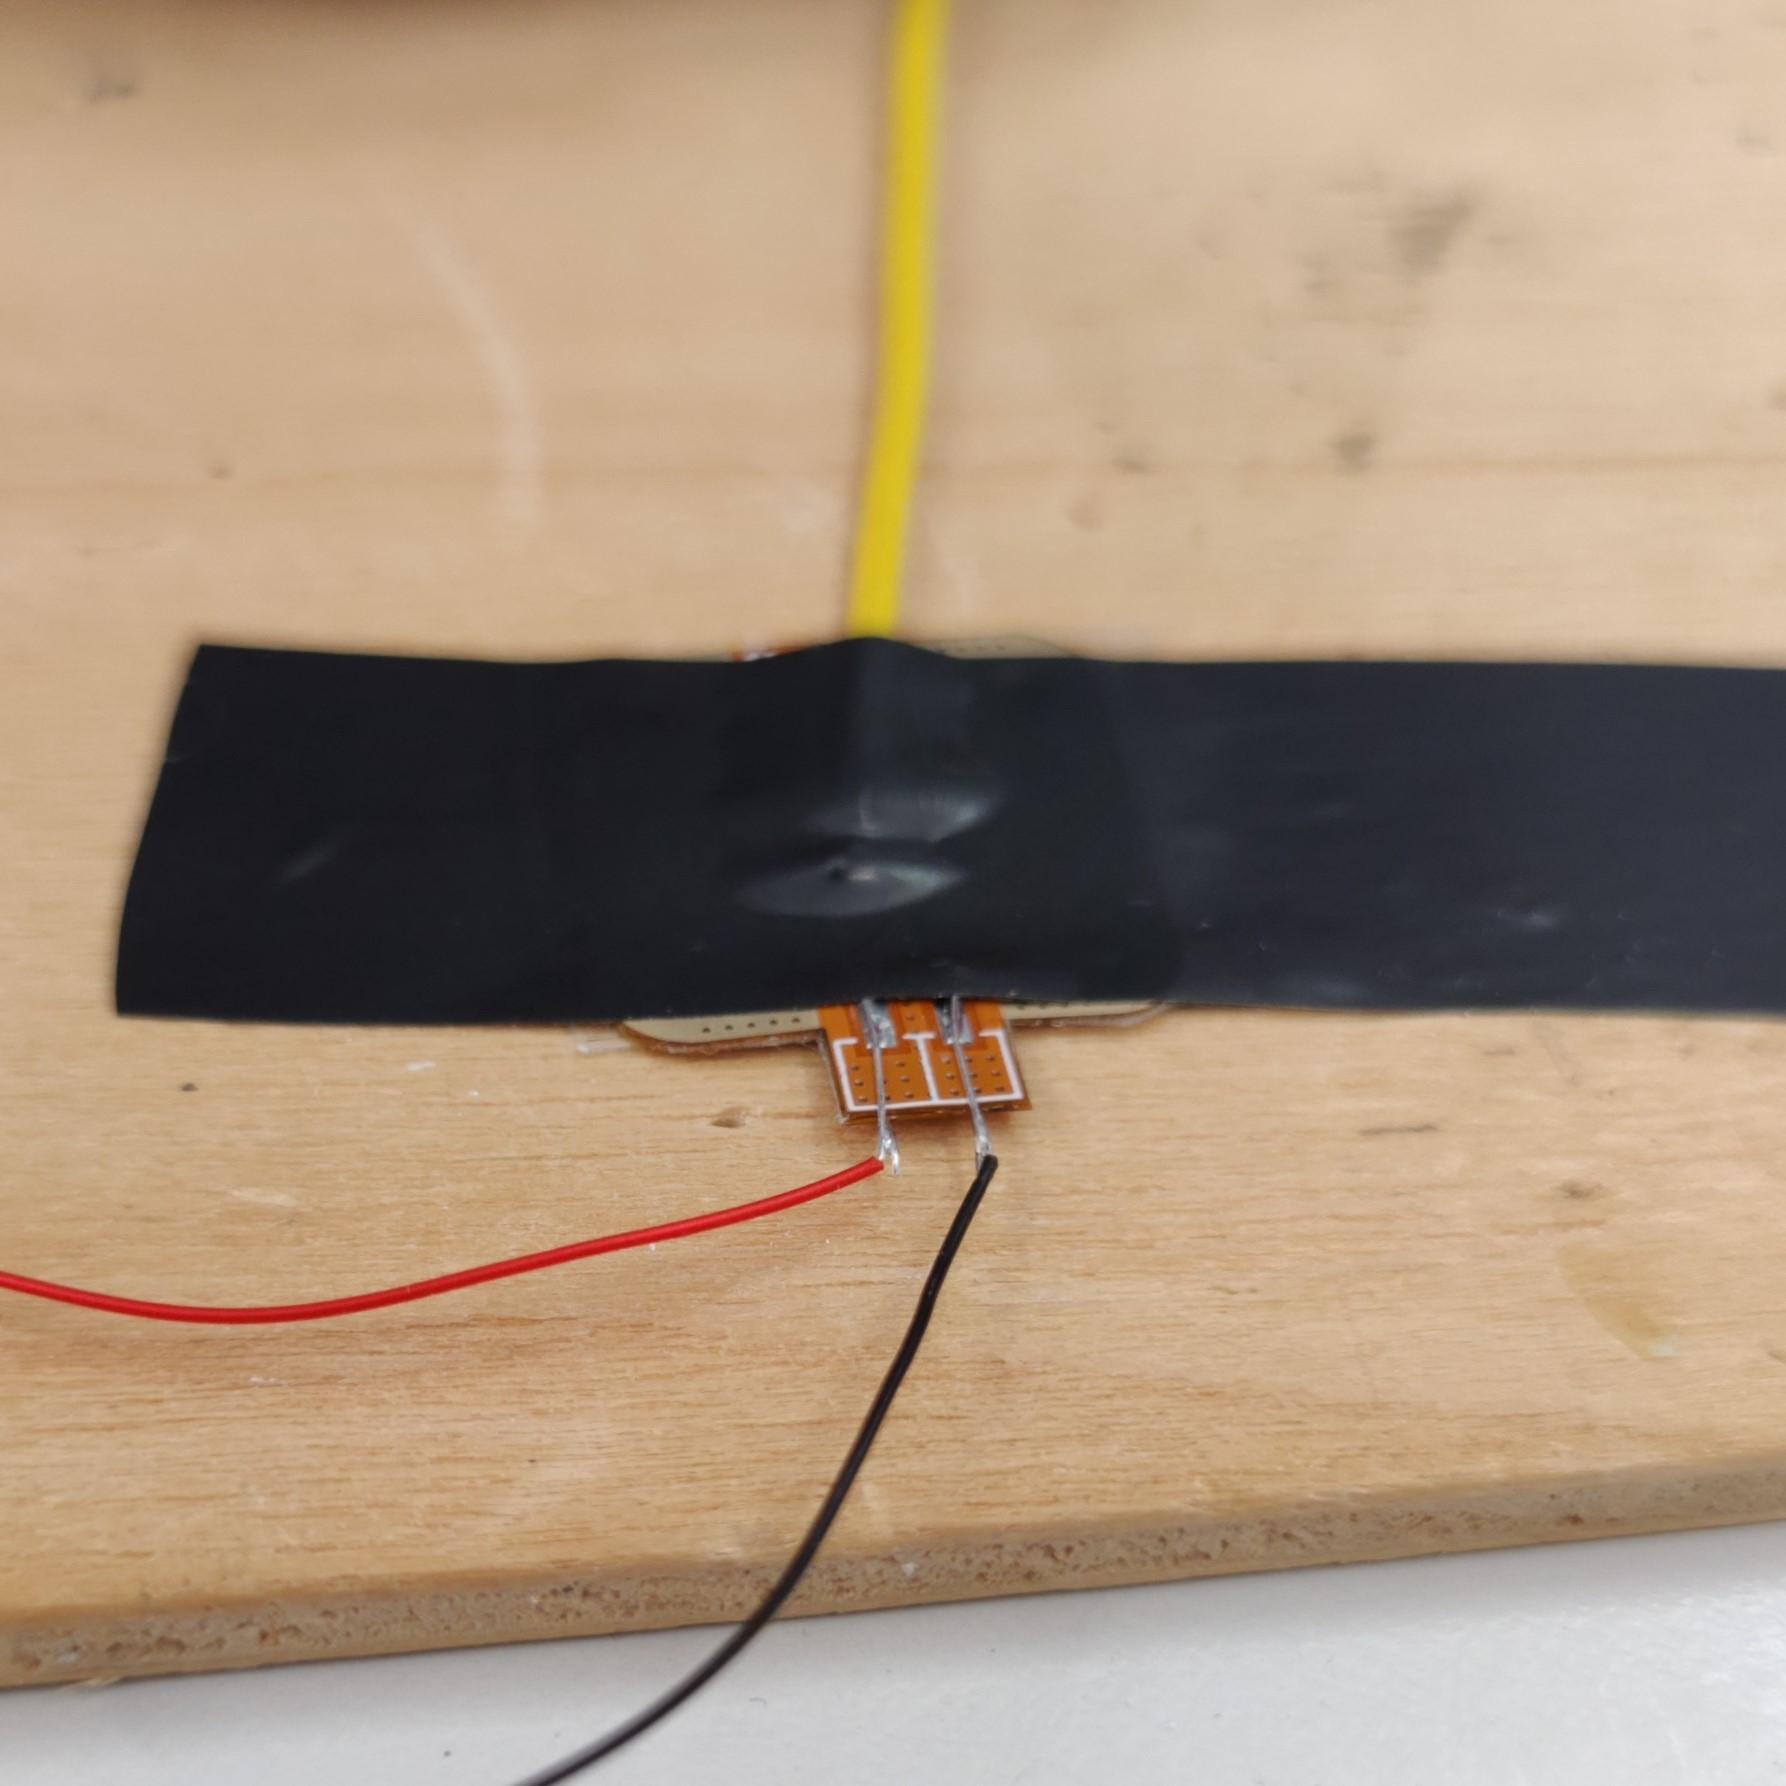
\includegraphics{Chapters/Chapter5/Exp_Evaluation/Figures/Heating_test_setup.jpg}
    }
    \caption{Heating test setup.}
    \label{fig: Heating_test_setup}
\end{figure}

\subsubsection{Single coil tests' results}
The results of the single coil tests are shown in figure \ref{fig: Single_coil_heating_tests}.
\begin{figure}
    \centering
    \resizebox{0.9\textwidth}{!}{
        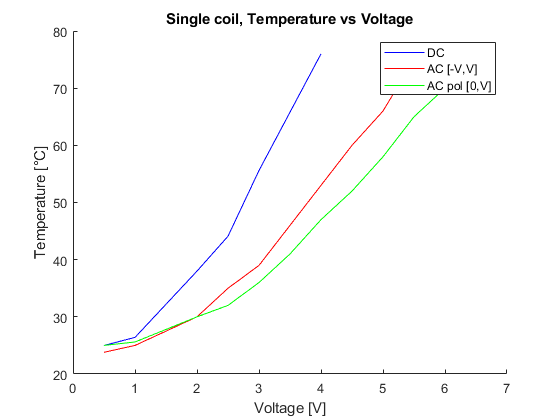
\includegraphics{Chapters/Chapter5/Exp_Evaluation/Figures/Temp_vs_Volt_1_coil.png}
    }
    \caption{Temperature vs Voltage for one coil.}
    \label{fig: Single_coil_heating_tests}
\end{figure}
As we can observe the coil tends to heat up way less in AC conditions, especially in the unipolar case.
This is due to the lower RMS value of the current that flows through the coil in AC conditions.

\subsubsection{Two coils in parallel tests' results}
The results of the two coils in parallel tests are shown in figure \ref{fig: Two_coils_heating_tests}.
\begin{figure}
    \centering
    \resizebox{0.9\textwidth}{!}{
        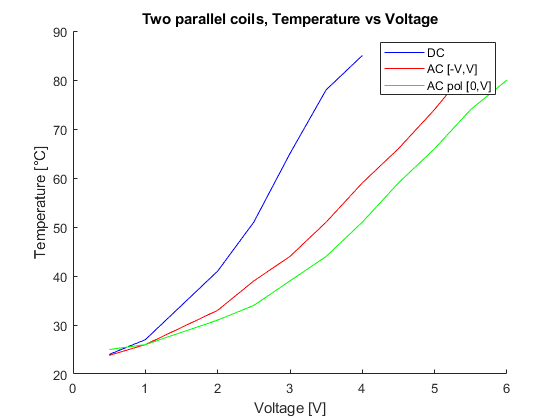
\includegraphics{Chapters/Chapter5/Exp_Evaluation/Figures/Temp_vs_Volt_2_coils.png}
    }
    \caption{Temperature vs Voltage for two coils in parallel.}
    \label{fig: Two_coils_heating_tests}
\end{figure}
This case is comparable to the previous one, but here the two coils in parallel tend to heat up more than the single coil even if the current is divided between the two coils.
This is because the two coils are glued together and the heat generated by one coil is transferred to the other one.

% -- Subsection 4.3
\subsection{Force testing}
The force testing was conducted on the flexible mat prototypes.
The goal of these tests was to understand the relationship between the force generated by the coil and the voltage applied to it.
To measure the force generated by the coil we used an ATI TW-Nano17 force sensor.
As we needed to measure the force in the z direction we had to create a way to suspend the sensor above the mat membrane.
This mount should also allow the sensor's position to be adjusted on the z-axis to be able to position the sensor at the right height to not press the membrane too much.
We modeled the structure based on the 3D model of the ATI sensor and then 3D printed its various components.

\begin{figure}
    \centering
    \resizebox{0.9\textwidth}{!}{
        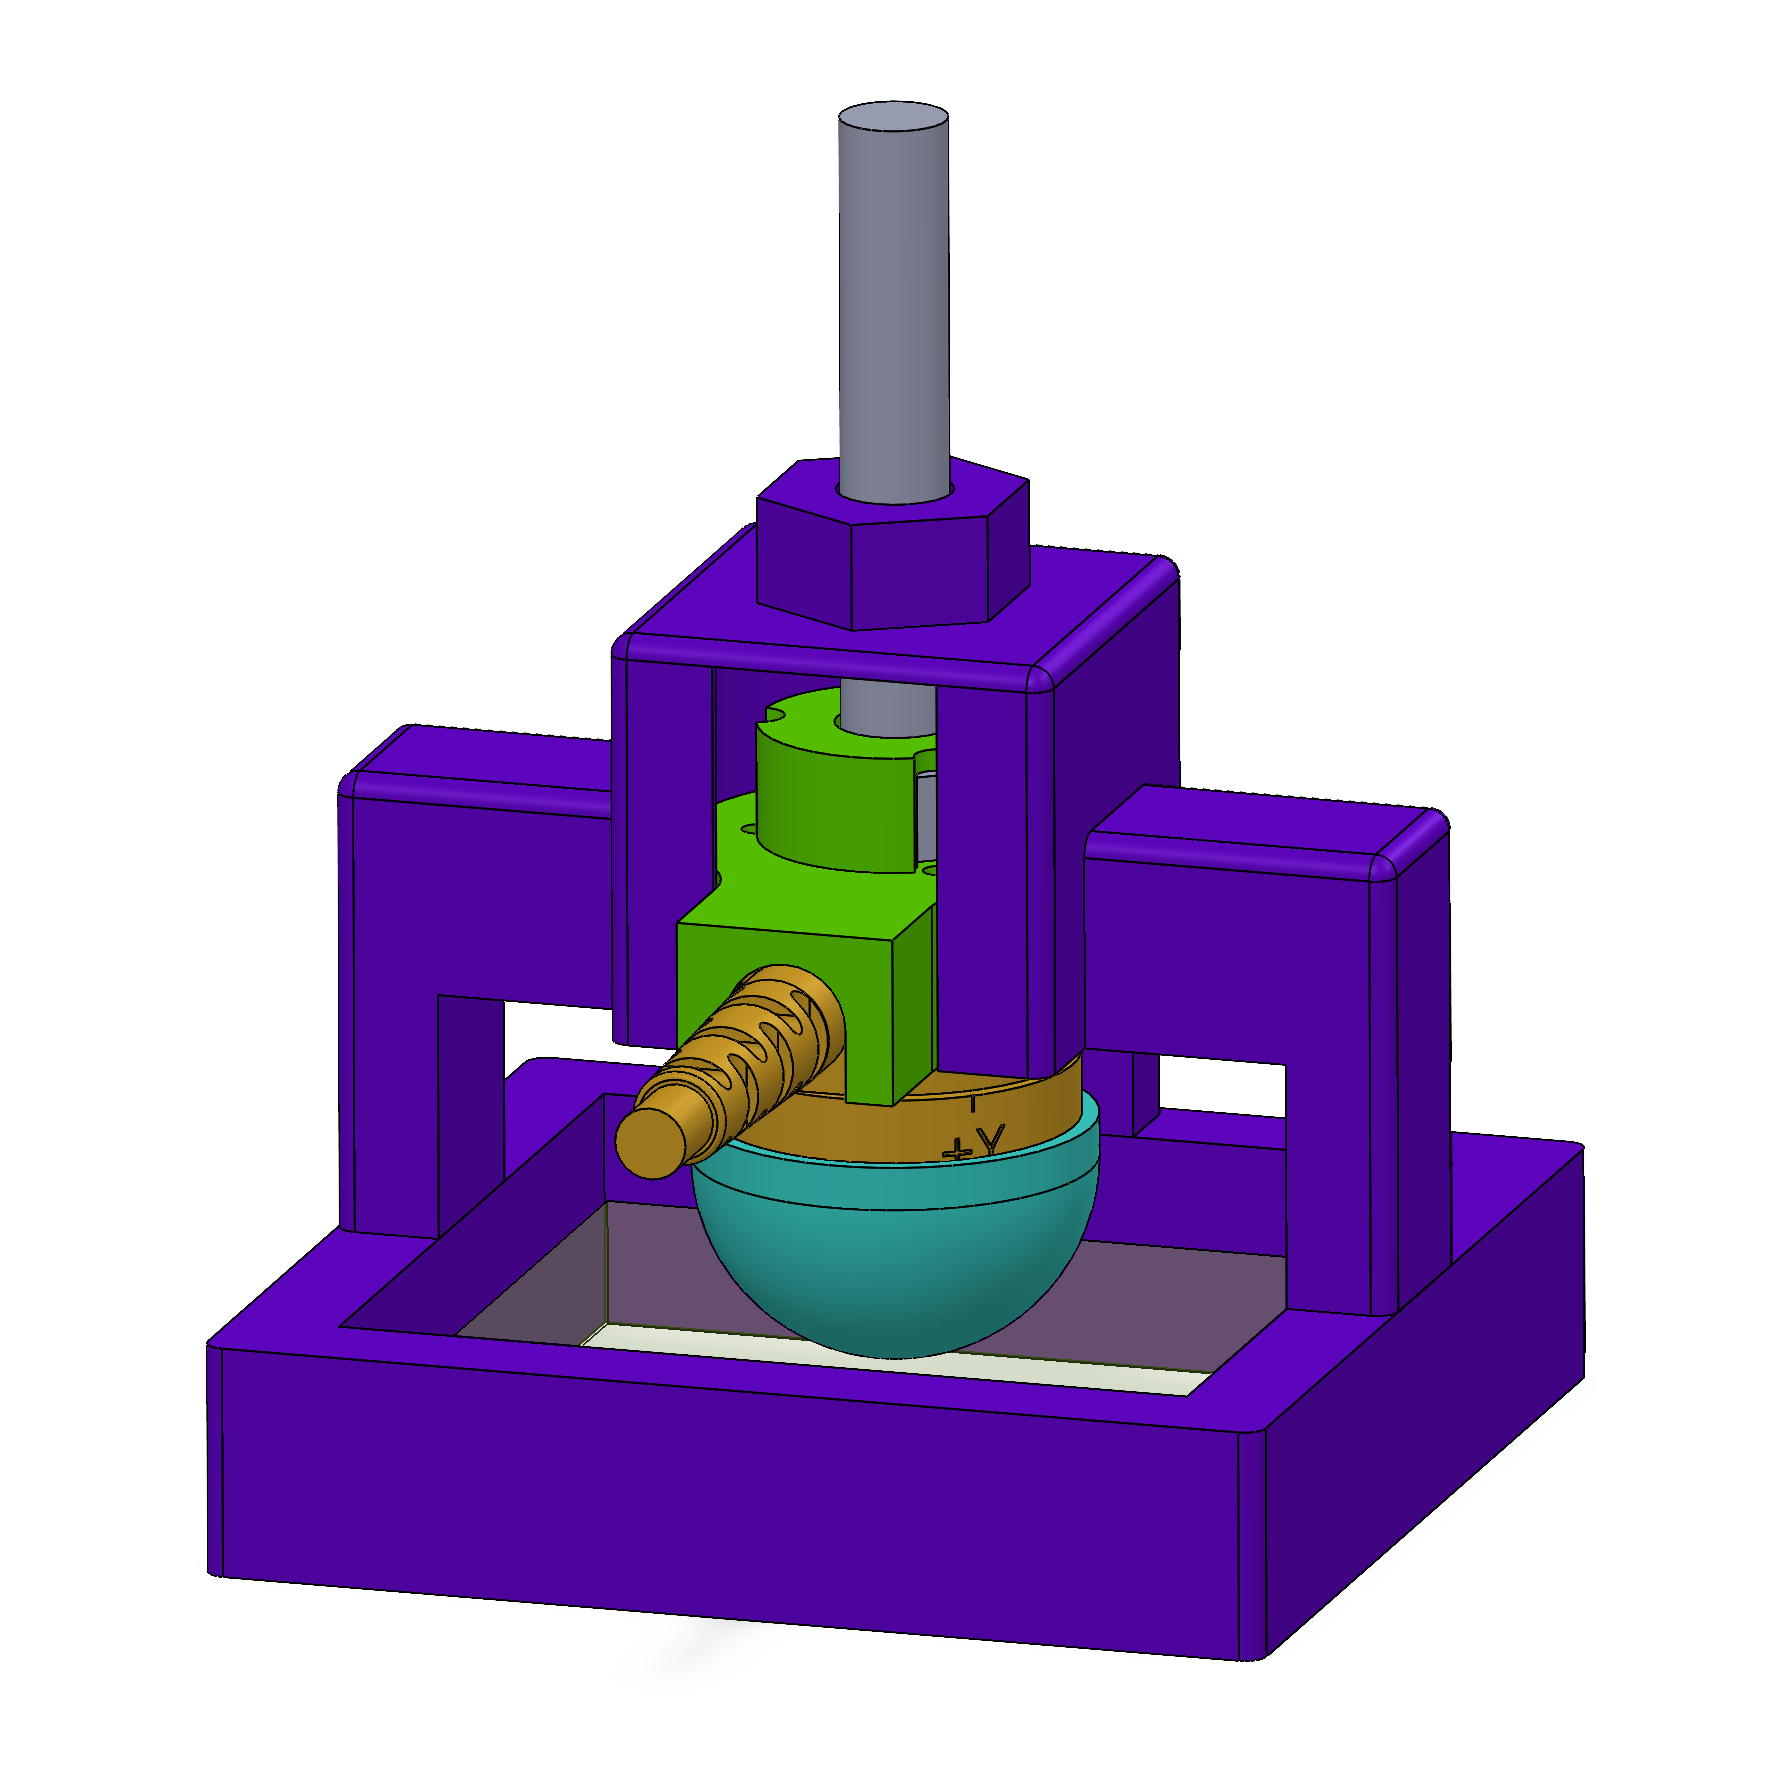
\includegraphics{Chapters/Chapter5/Exp_Evaluation/Figures/ATI_test_platform.png}
    }
    \caption{Sensor mount complete structure.}
    \label{fig: Sensor_mount_complete}
\end{figure}

The structure is composed of 3 3D printed PLA components, one nut and a bolt.
The components are the following:
\begin{itemize}
    \item \textbf{Sensor mount:} this component holds the sensor and houses the bolt head on its top. It was designed to trap the head of the bolt but to leave it able to rotate, this was done by temporarily pausing the printing process and inserting the bolt. Then the printing process was resumed to create the blocking layers on the bottom of the bolt's head. (Green component in figure \ref{fig: Sensor_mount_complete})
    \begin{figure}
        \centering
        \resizebox{0.9\textwidth}{!}{
            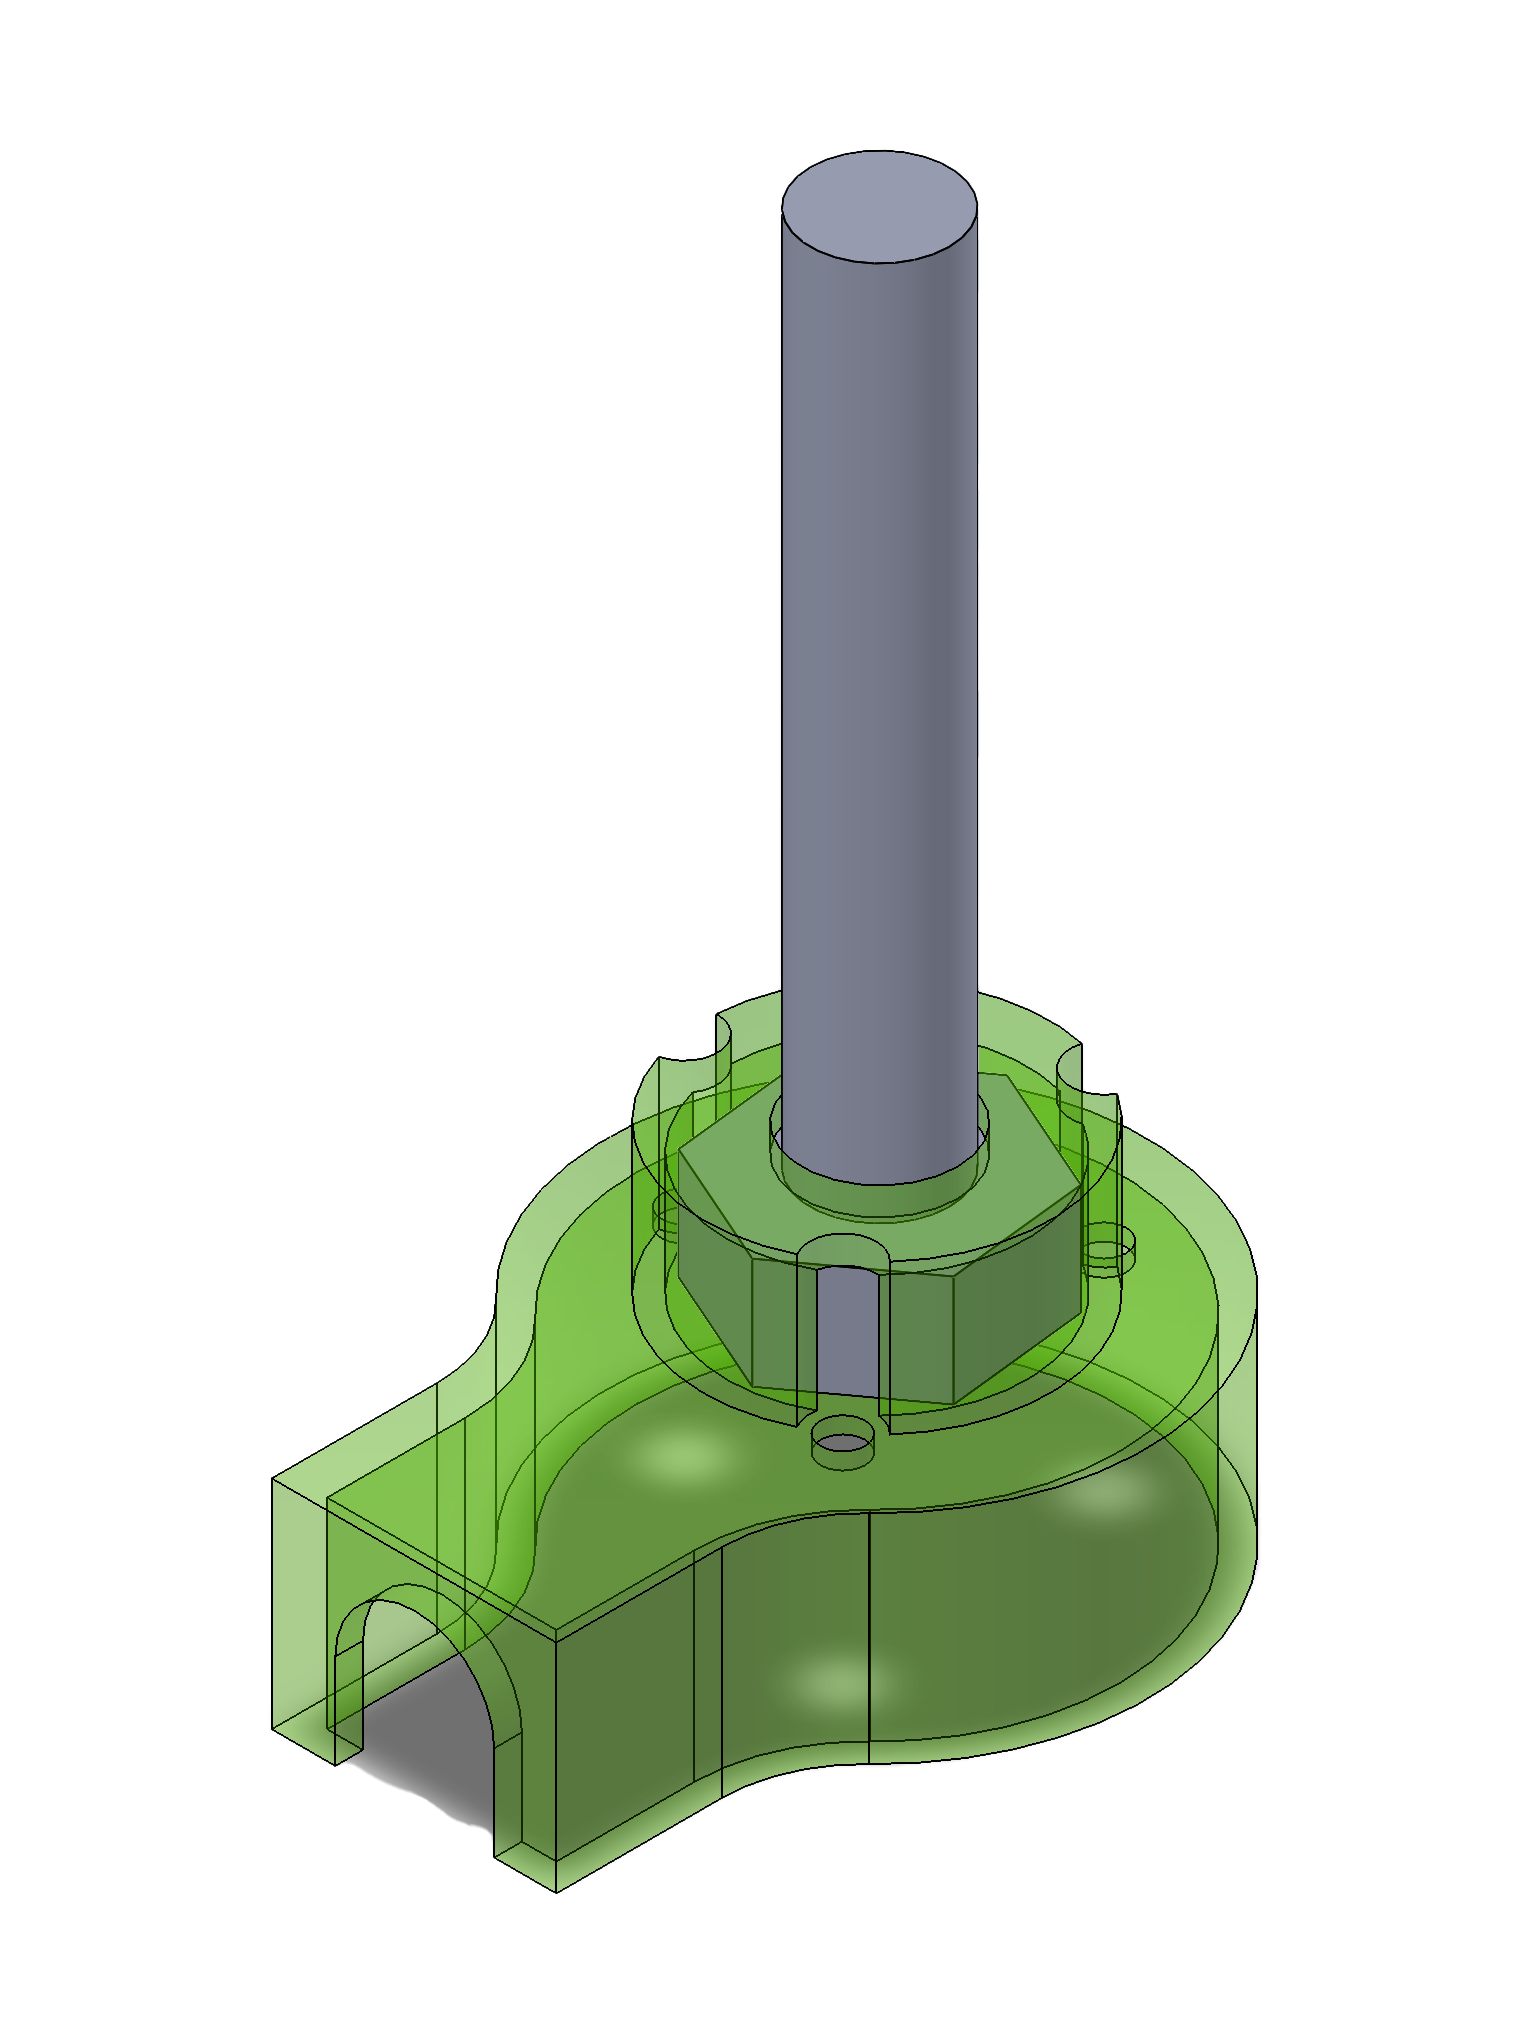
\includegraphics{Chapters/Chapter5/Exp_Evaluation/Figures/ATI_grabber.png}
        }
        \caption{Sensor mount see-through view.}
        \label{fig: Sensor_mount}
    \end{figure}

    \item \textbf{Sensor mount base:} this component is the base of the structure, on the bottom has a squared hole where the flexible mat can be inserted and on the top houses a nut trapped in the print to allow the bolt to be screwed up and down. (Purple component in figure \ref{fig: Sensor_mount_complete})
    \begin{figure}
        \centering
        \resizebox{0.9\textwidth}{!}{
            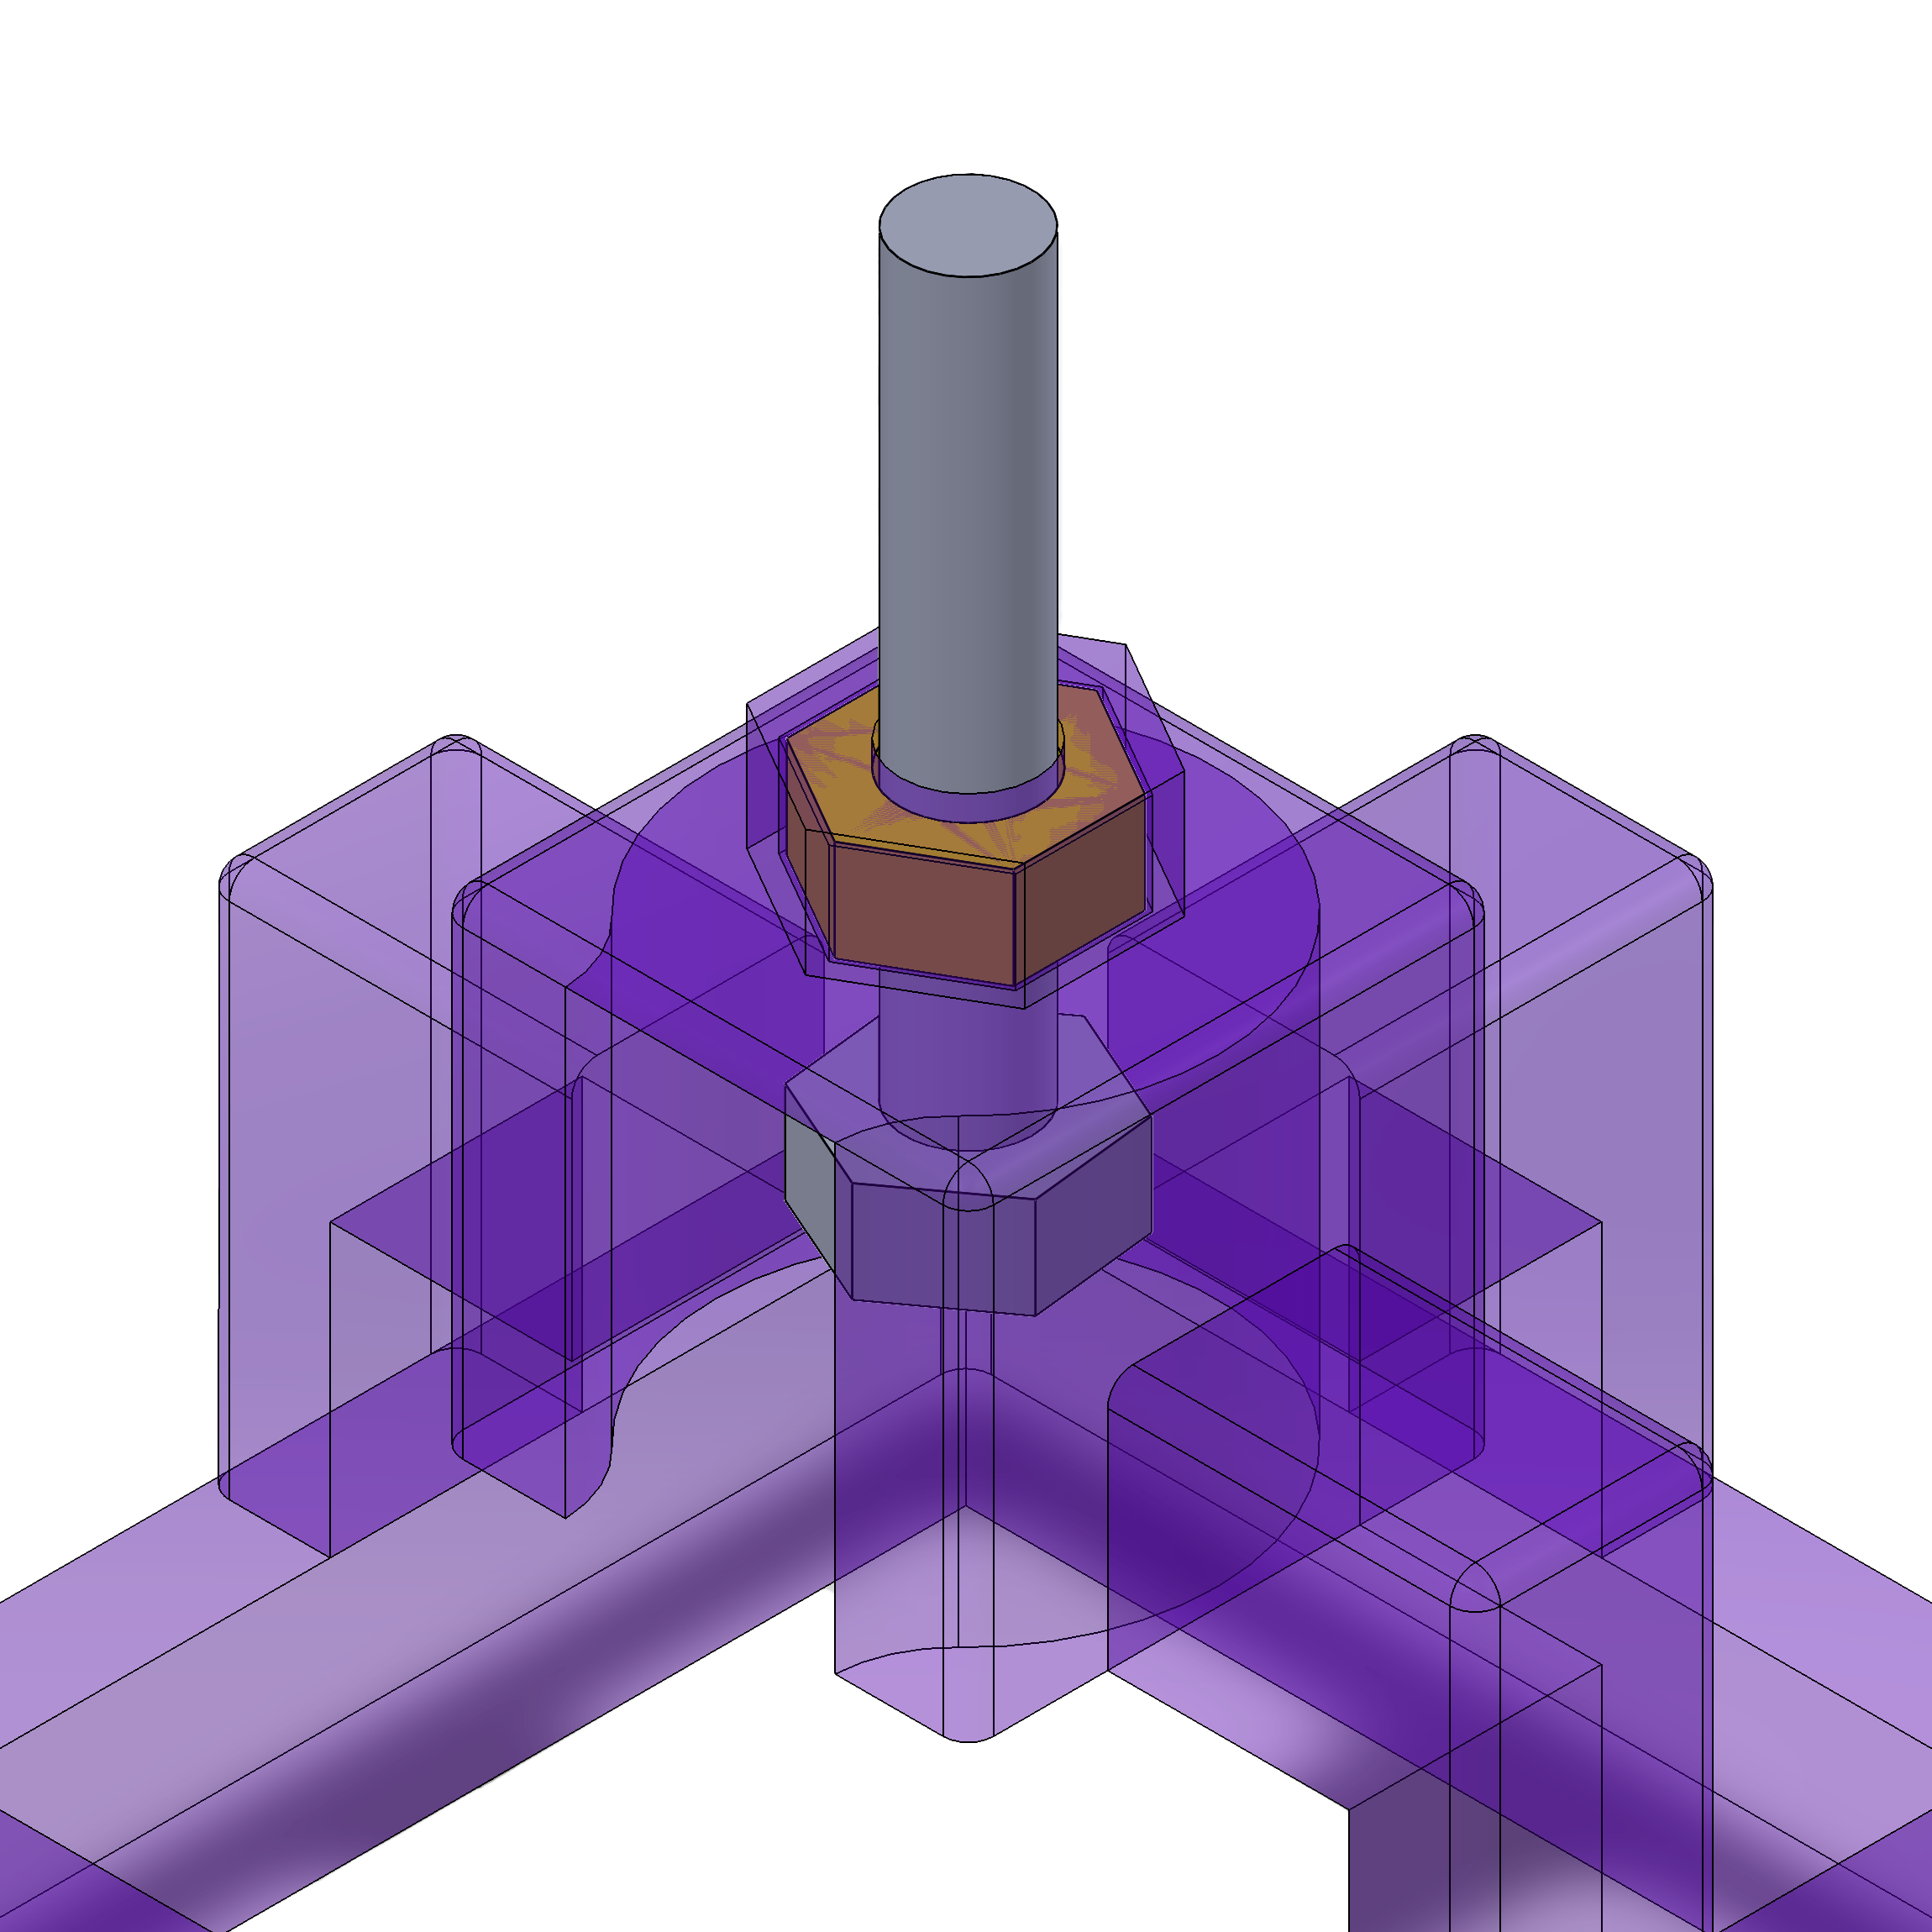
\includegraphics{Chapters/Chapter5/Exp_Evaluation/Figures/ATI_platform_mech.png}
        }
        \caption{Sensor mount base see-through view of the nut and bolt mechanism.}
    \end{figure}

    \item \textbf{Sensor's pulp:} this component is mounted below the sensor and is used to press the membrane of the mat on a small area, to simulate a finger pressing on the mat. (Teal component in figure \ref{fig: Sensor_mount_complete})

\end{itemize}

The complete test setup is shown in figure \ref{fig: Force_test_setup}.
\begin{figure}
    \centering
    \resizebox{0.9\textwidth}{!}{
        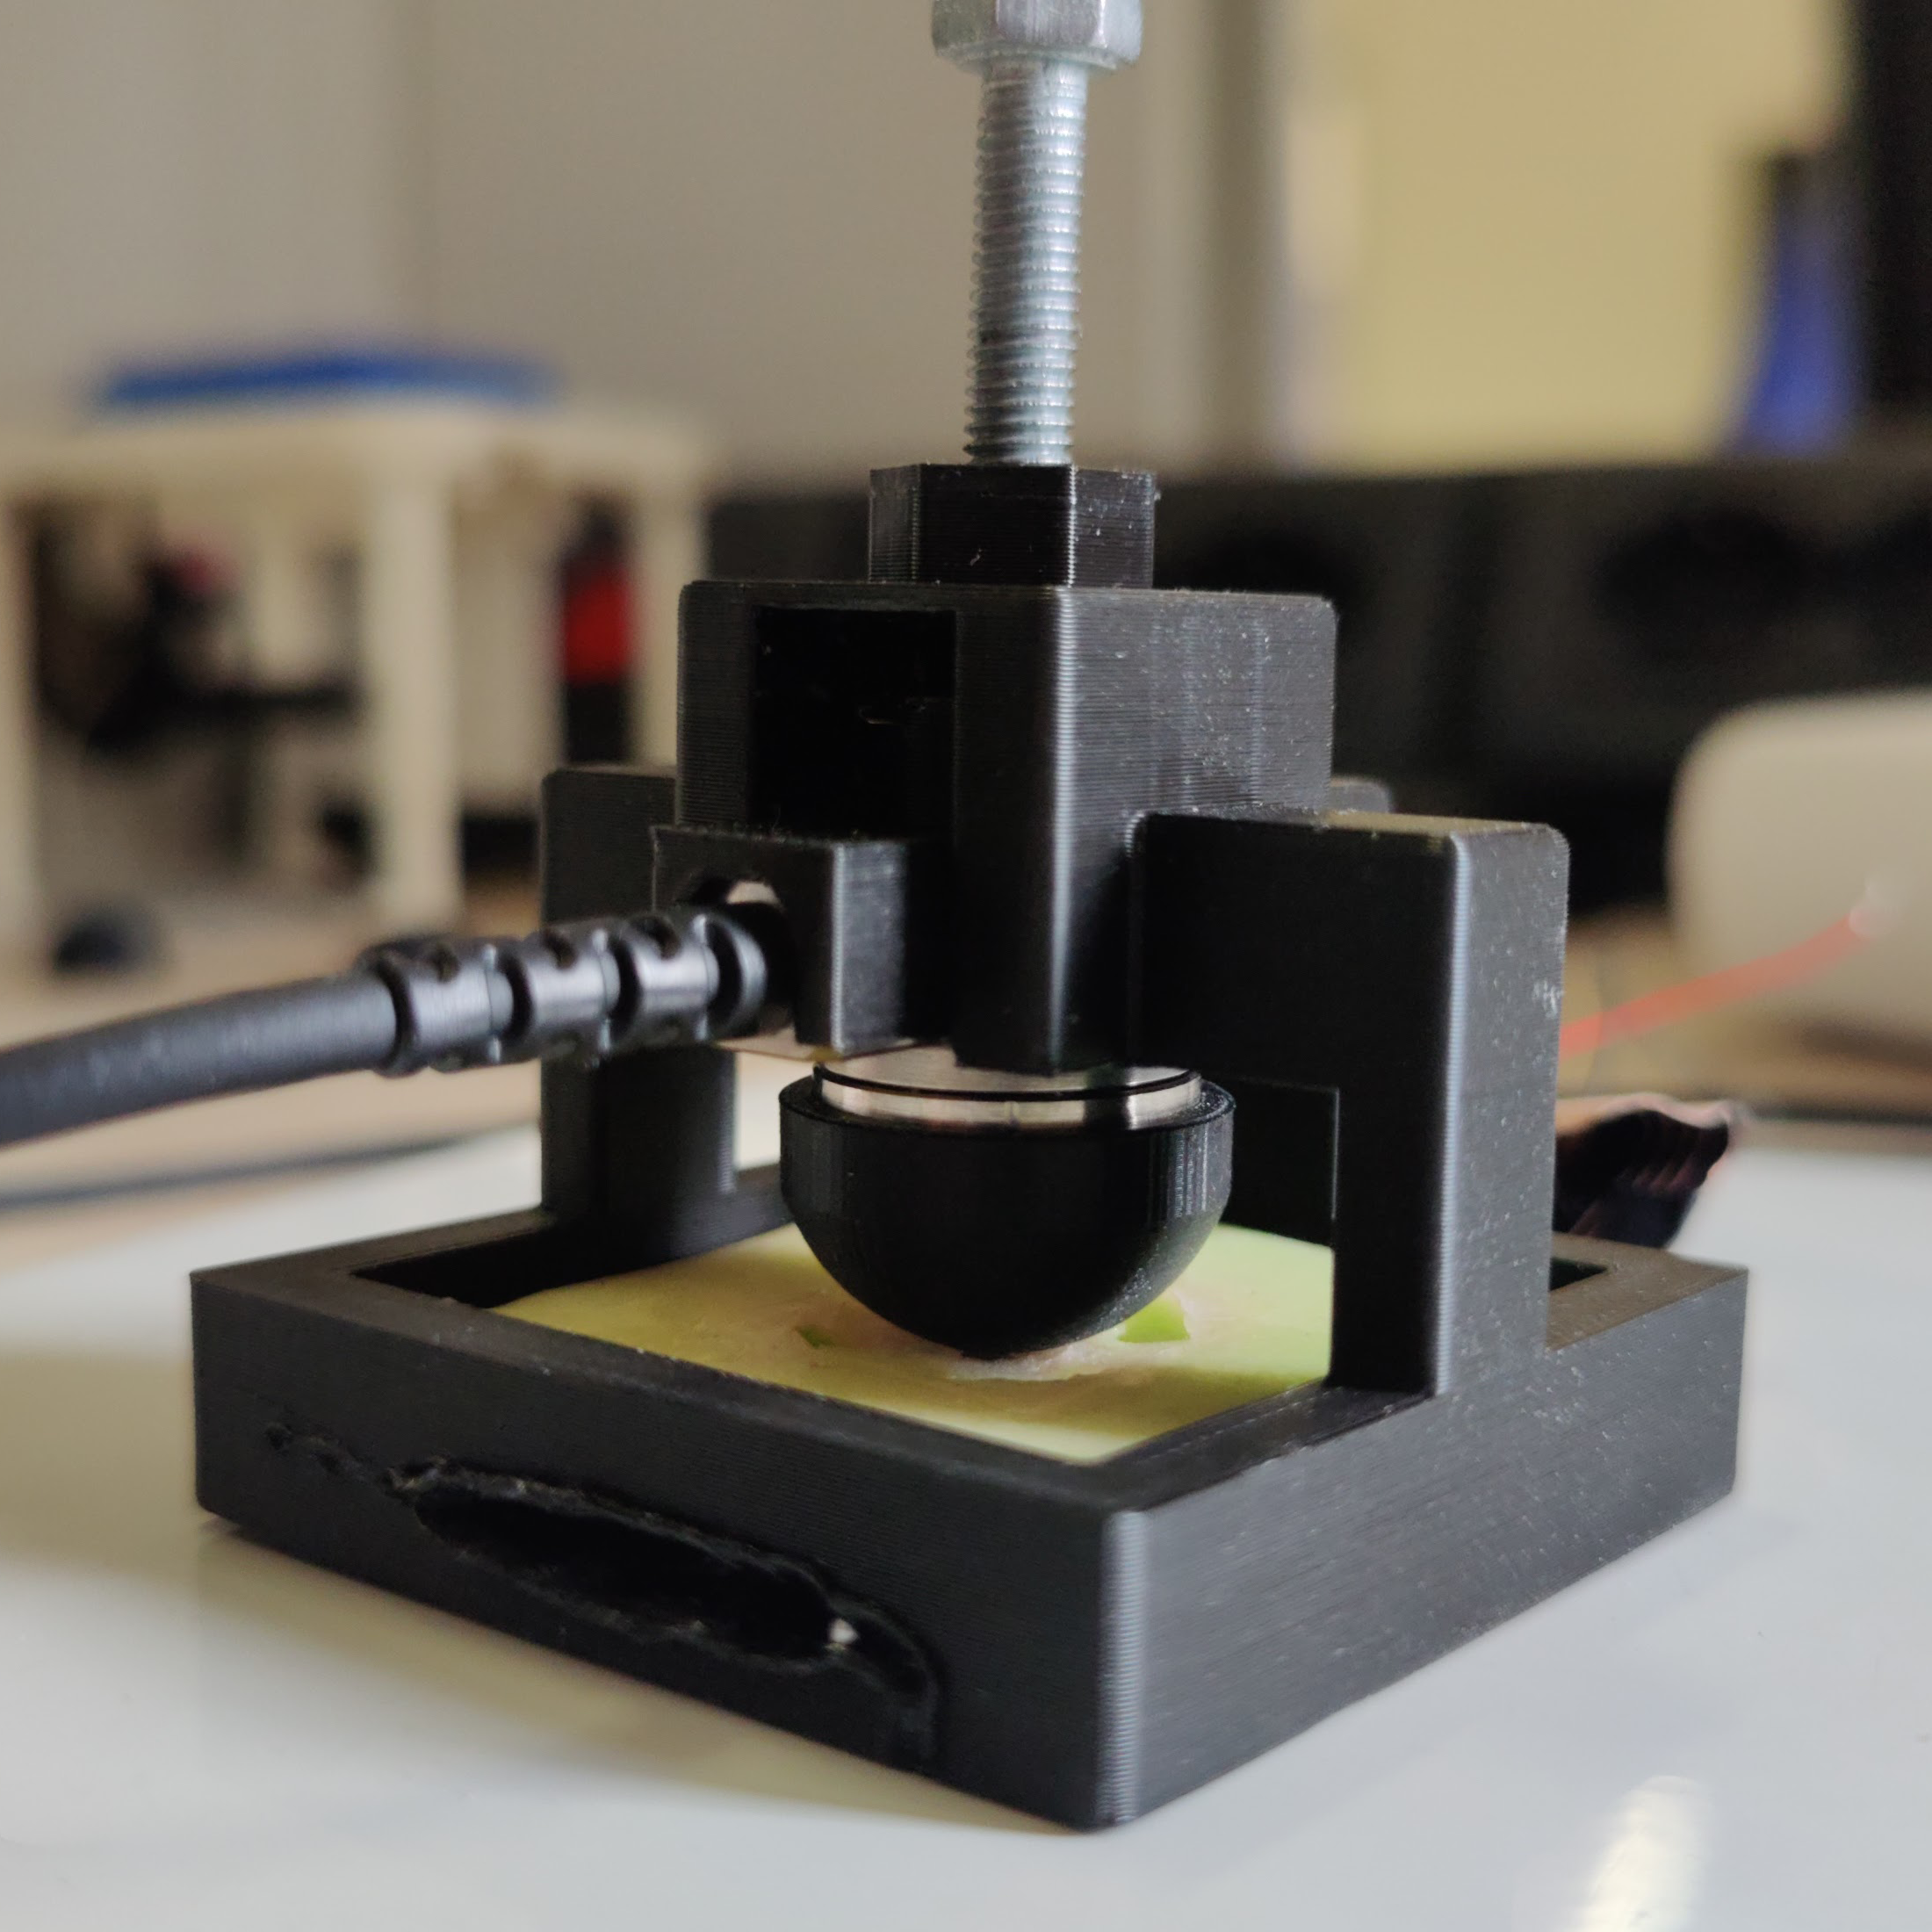
\includegraphics{Chapters/Chapter5/Exp_Evaluation/Figures/ATI_mat_complete.png}
    }
    \caption{Complete force testing setup.}
    \label{fig: Force_test_setup}
\end{figure}

ATI data acquisition was done with a MATLAB script based on the work of \cite{ATI_NetFT_MatlabInterface}.

\subsubsection{ATI sensor low sensitivity}
After some tests, we quickly realized that the ATI sensor was not sensitive enough to measure the forces generated by the mat prototype when driven with sinusoidal signals.
This is because, even at the max rated voltage we can drive the coil with (6V), the magnetic field generated by the coil is not strong enough to generate a magnetic repulsion force with the magnet that can be measured by the sensor.
The only way to measure the force generated by the coil is to make it produce a way higher magnetic field, the solution we found was to use a signal with very high peaks but low RMS voltage.
In this way, the coil can generate high peaks of magnetic field for a short time, enough to generate a force that can be measured by the sensor.
A good candidate for testing with this type of signals is the heartbeat pulse, it presents a very high peak at the ventricles contraction and then a low value during the rest of the heartbeat cycle.
\begin{figure}
    \centering
    \resizebox{0.9\textwidth}{!}{
        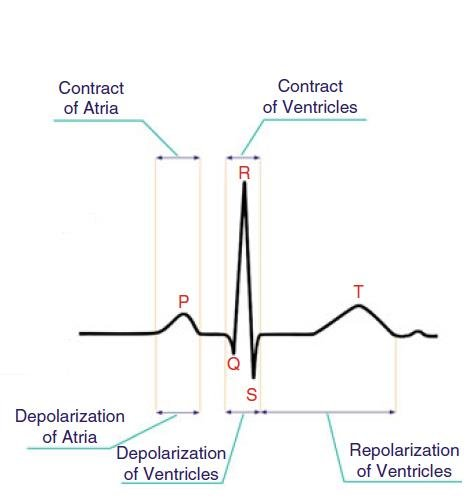
\includegraphics{Chapters/Chapter5/Exp_Evaluation/Figures/heartbeat_pulse.png}
    }
    \caption{Heartbeat pulse.}
    \label{fig: Heartbeat_pulse}
\end{figure}
We chose the heartbeat because it's a good example for our case study as it is a low-frequency signal and because we managed to run the coil with it even at up to 30V peak value without reaching its thermal runaway point.
Also, the simulated heartbeat was easily recognizable by the subjects who tested the flexible mat prototype.

\subsubsection{Testing procedure}
To measure the force generated by the mat prototypes we used an automatic testing procedure controlled by a MATLAB script.
The computer running the script was connected to the function generator and the ATI sensor.
The script was designed to:
\begin{itemize}
    \item Set the function generator to output the desired signal, voltage and frequency.
    \item Measure the force offset on the sensor when the coil was off.
    \item Turn on the signal on the function generator.
    \item Read the sensor data for a given amount of seconds, with a given number of samples.
    \item Turn off the signal.
\end{itemize}
Then the script would plot the force data and save it to a file.

\subsubsection{Magnet size vs Force}
The main reason we decided to carry out this test was to compare the force generated by the two mat prototypes we developed, the one with the small magnet and the one with the big magnet.
We tested them both using two coils in parallel and the heartbeat pulse signal at 30V peak value.

The results of the tests are shown in figure \ref{fig: Force_vs_magnet_size}.
\begin{figure}
    \centering
    \begin{subfigure}[b]{0.475\textwidth}
        \centering
        \resizebox{0.9\textwidth}{!}{
            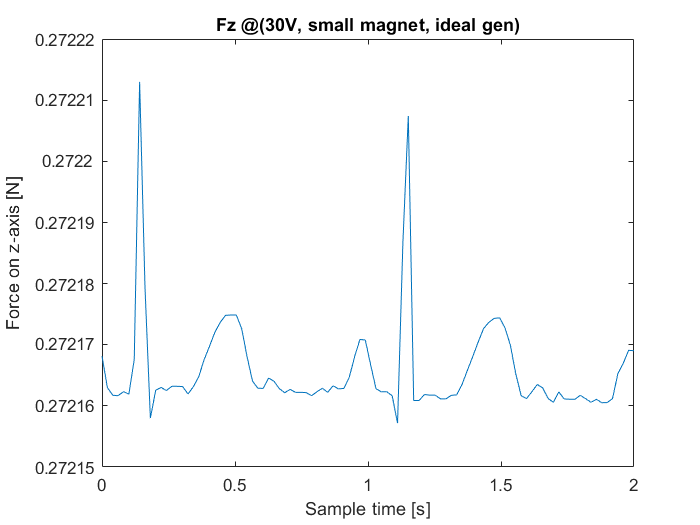
\includegraphics{Chapters/Chapter5/Exp_Evaluation/Figures/Fz_@30V_small_magn_idealgen.png}
        }
        \caption{Force profile of the small magnet prototype.}
    \end{subfigure}
    \begin{subfigure}[b]{0.475\textwidth}
        \centering
        \resizebox{0.9\textwidth}{!}{
            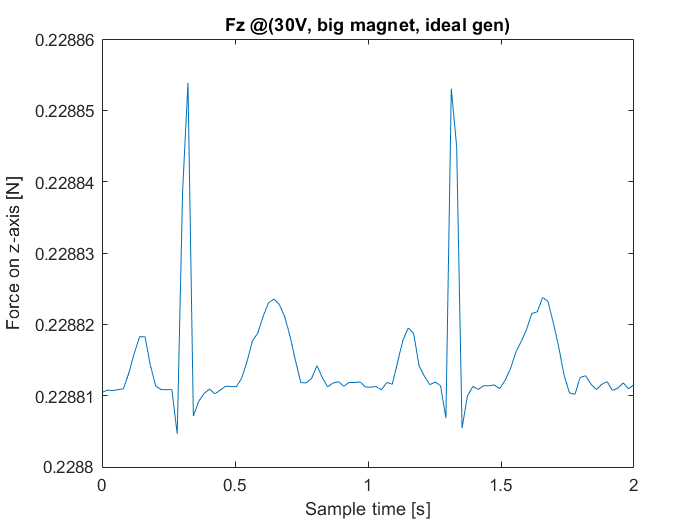
\includegraphics{Chapters/Chapter5/Exp_Evaluation/Figures/Fz_@30V_big_magn_idealgen.png}
        }
        \caption{Force profile of the big magnet prototype.}
    \end{subfigure}
    \caption{Force profile of the two mat prototypes run with the heartbeat pulse signal.}
    \label{fig: Force_vs_magnet_size}
\end{figure}

As we can see the force generated by the two prototypes is comparable, but sadly the force generated by the big magnet prototype is lower than the one generated by the small magnet prototype.

 

\chapter{Discussion and conclusions}
\label{Chapter6}
%----------------------------------------------------------------------------------------
%	SECTION 1
%----------------------------------------------------------------------------------------
    
\section{Challenges in On-Board AI Systems for Space Missions}

AI algorithms in on-board space applications encounter significant challenges related to both verifiability and computational load, crucial factors for the success and safety of space missions.

\subsection{Verifiability Issues}
AI algorithms, particularly those employing deep learning, are characterized by intricate architectures and numerous parameters. The complexity of these models makes it challenging to provide comprehensive assurance of their correctness. In space applications, where system failures are not an option, ensuring the verifiability of AI algorithms becomes predominant.

Many AI models, including deep neural networks, lack inherent explainability. Understanding the decision-making process within these "black box" models is essential to verify their reliability. Achieving transparency in AI decision logic is critical in scenarios where the basis for decision-making must be interpretable, such as during critical space maneuvers.

Space environments are dynamic and may exhibit uncertainties. AI algorithms designed for adaptability and learning might introduce challenges in predicting their behavior accurately. Verifying the robustness of adaptive AI systems in the face of unforeseen conditions is a persistent concern.

\subsection{Computational Issues}
On-board space systems typically operate with limited computational resources due to factors such as size, weight, and power constraints (SWaP). Implementing AI algorithms with demanding computational requirements may strain available resources, affecting the overall efficiency of the system.

Certain space applications, such as autonomous navigation or hazard avoidance, demand real-time decision-making. AI algorithms with high computational loads may struggle to meet these stringent timing constraints. Delays in processing could lead to missed opportunities or, in critical situations, mission failure.

In addition to computational power, energy efficiency is a crucial consideration. Prolonged missions and the reliance on energy-harvesting sources necessitate AI algorithms that balance computational complexity with energy consumption, ensuring sustained and reliable operation.

Addressing these challenges requires a multidisciplinary approach involving AI researchers, space engineers, and mission planners. Techniques such as formal verification, explainable AI, and hardware optimization are essential to enhance the verifiability and efficiency of AI algorithms in on-board space applications.

\section{Results Analysis}
In the broader context, the multi-model configuration emerges as the more robust and adaptable option, showcasing superior performance on the test set and demonstrating effective generalization capabilities to previously unseen data. The overall system score on the test dataset is $S$ = 0.0447, primarily affected by the translation component $S_T$ = 0.0390, as opposed to the relatively lower contribution from the rotation aspect, $S_R$ = 0.0057. The noteworthy aspect is the necessity of prioritize the minimization of translation errors, since, in proximity to the target, precise translation is crucial for accurate maneuvering.
Moreover, rotation pose can be more effectively predicted with the incorporation of a navigation filter. This strategic integration allows for a corrective mechanism, compensating for rotational discrepancies and enhancing the system's overall precision in navigating close quarters.

\section{Possible Improvements}
\label{Chapter6/Improv}


Another option would be using multiple models also for the \textit{Landmark Regression} module, which are able to identify a target set of landmarks in farther positions and a second set in closer distances to the target, in order to keep the number of identified points in the image frame as greater as possible.\\
This implementation would also lead to a more accurate pose estimation in positions closer to the minimum distance analyzed in the experiments (from $40 cm$ to $20cm$). A well-performed pose estimation in positions very close to the target would help to minimize any errors introduced by camera distortions.

\subsection{Landmark Mapping Sensitivity}
The assessment of trajectories such as \textit{Less\_Difficult\_Trajectory} and \textit{Difficult\_Trajectory} is conducted with a noteworthy consideration: the assumption of zero prediction error for the points' location in the image. This assumption is made out of necessity since the \textit{Landmark Regression} module encounters difficulties in identifying all the landmarks expected to be present in the image frames. Consequently, the input data for the \textit{Landmark Mapping} module is marked by a heightened sensitivity, as the accuracy of its predictions is contingent upon the successful identification of landmarks by the preceding module.

A potential avenue for improvement involves an expansion of the training dataset to incorporate instances where certain landmarks remain unidentified due to inherent challenges in their recognition. This strategy aims to enhance the model's resilience to scenarios where specific landmarks pose persistent issues during identification. By exposing the model to a more diverse range of challenges and including cases of landmark ambiguity, it is anticipated that the trained model will develop a more robust understanding, leading to improved performance, particularly in situations mirroring real-world complexities. This adjustment aligns with the overarching goal of fortifying the system's adaptability and generalization capabilities, addressing challenges posed by varying environmental conditions and unforeseen factors during autonomous space applications.

Moreover, to fortify the robustness of the system, there is a prospect to introduce a more sophisticated pre-processing system. This advanced system would be designed to mitigate the impact of varying image light conditions on landmark identification. By incorporating techniques such as adaptive image enhancement, contrast normalization, or even exploring deep learning-based methods for illumination invariance, the model could become less susceptible to fluctuations in lighting. Such enhancements would foster greater reliability in landmark identification by the \textit{Landmark Regression} module, subsequently improving the overall accuracy of the \textit{Landmark Mapping} module. This proactive approach anticipates and addresses challenges associated with real-world scenarios where illumination conditions can be unpredictable, ensuring the model's effectiveness across diverse operational environments in on-board space applications.

\section{Conclusions}
This project presents a dedicated monocular pose estimation framework designed for spaceborne objects, emphasizing its applicability to satellite rendezvous maneuvers. The framework capitalizes on the strengths of deep neural networks, seamlessly integrating feature learning and establishing robust 2D-3D correspondence mapping. Notably, the incorporation of HRNet, known for its high-resolution image representation, significantly contributes to the precision of pose predictions and the subsequent refinement process. The framework further demonstrates its efficiency by employing geometric optimization techniques, ensuring accurate alignment of point sets and enhancing the overall robustness of the pose estimation system.
%% Chapter 1

\chapter{Chapter Title Here} % Main chapter title

\label{Chapter1} % For referencing the chapter elsewhere, use \ref{Chapter1} 

%----------------------------------------------------------------------------------------

% Define some commands to keep the formatting separated from the content 
\newcommand{\keyword}[1]{\textbf{#1}}
\newcommand{\tabhead}[1]{\textbf{#1}}
\newcommand{\code}[1]{\texttt{#1}}
\newcommand{\file}[1]{\texttt{\bfseries#1}}
\newcommand{\option}[1]{\texttt{\itshape#1}}

%----------------------------------------------------------------------------------------

\section{Welcome and Thank You}
Welcome to this \LaTeX{} Thesis Template, a beautiful and easy to use template for writing a thesis using the \LaTeX{} typesetting system.

If you are writing a thesis (or will be in the future) and its subject is technical or mathematical (though it doesn't have to be), then creating it in \LaTeX{} is highly recommended as a way to make sure you can just get down to the essential writing without having to worry over formatting or wasting time arguing with your word processor. 

\LaTeX{} is easily able to professionally typeset documents that run to hundreds or thousands of pages long. With simple mark-up commands, it automatically sets out the table of contents, margins, page headers and footers and keeps the formatting consistent and beautiful. One of its main strengths is the way it can easily typeset mathematics, even \emph{heavy} mathematics. Even if those equations are the most horribly twisted and most difficult mathematical problems that can only be solved on a super-computer, you can at least count on \LaTeX{} to make them look stunning.

%----------------------------------------------------------------------------------------

\section{Learning \LaTeX{}}

\LaTeX{} is not a \textsc{wysiwyg} (What You See is What You Get) program, unlike word processors such as Microsoft Word or Apple's Pages. Instead, a document written for \LaTeX{} is actually a simple, plain text file that contains \emph{no formatting}. You tell \LaTeX{} how you want the formatting in the finished document by writing in simple commands amongst the text, for example, if I want to use \emph{italic text for emphasis}, I write the \verb|\emph{text}| command and put the text I want in italics in between the curly braces. This means that \LaTeX{} is a \enquote{mark-up} language, very much like HTML.

\subsection{A (not so short) Introduction to \LaTeX{}}

If you are new to \LaTeX{}, there is a very good eBook -- freely available online as a PDF file -- called, \enquote{The Not So Short Introduction to \LaTeX{}}. The book's title is typically shortened to just \emph{lshort}. You can download the latest version (as it is occasionally updated) from here:
\url{http://www.ctan.org/tex-archive/info/lshort/english/lshort.pdf}

It is also available in several other languages. Find yours from the list on this page: \url{http://www.ctan.org/tex-archive/info/lshort/}

It is recommended to take a little time out to learn how to use \LaTeX{} by creating several, small `test' documents, or having a close look at several templates on:\\ 
\url{http://www.LaTeXTemplates.com}\\ 
Making the effort now means you're not stuck learning the system when what you \emph{really} need to be doing is writing your thesis.

\subsection{A Short Math Guide for \LaTeX{}}

If you are writing a technical or mathematical thesis, then you may want to read the document by the AMS (American Mathematical Society) called, \enquote{A Short Math Guide for \LaTeX{}}. It can be found online here:
\url{http://www.ams.org/tex/amslatex.html}
under the \enquote{Additional Documentation} section towards the bottom of the page.

\subsection{Common \LaTeX{} Math Symbols}
There are a multitude of mathematical symbols available for \LaTeX{} and it would take a great effort to learn the commands for them all. The most common ones you are likely to use are shown on this page:
\url{http://www.sunilpatel.co.uk/latex-type/latex-math-symbols/}

You can use this page as a reference or crib sheet, the symbols are rendered as large, high quality images so you can quickly find the \LaTeX{} command for the symbol you need.

\subsection{\LaTeX{} on a Mac}
 
The \LaTeX{} distribution is available for many systems including Windows, Linux and Mac OS X. The package for OS X is called MacTeX and it contains all the applications you need -- bundled together and pre-customized -- for a fully working \LaTeX{} environment and work flow.
 
MacTeX includes a custom dedicated \LaTeX{} editor called TeXShop for writing your `\file{.tex}' files and BibDesk: a program to manage your references and create your bibliography section just as easily as managing songs and creating playlists in iTunes.

%----------------------------------------------------------------------------------------

\section{Getting Started with this Template}

If you are familiar with \LaTeX{}, then you should explore the directory structure of the template and then proceed to place your own information into the \emph{THESIS INFORMATION} block of the \file{main.tex} file. You can then modify the rest of this file to your unique specifications based on your degree/university. Section \ref{FillingFile} on page \pageref{FillingFile} will help you do this. Make sure you also read section \ref{ThesisConventions} about thesis conventions to get the most out of this template.

If you are new to \LaTeX{} it is recommended that you carry on reading through the rest of the information in this document.

Before you begin using this template you should ensure that its style complies with the thesis style guidelines imposed by your institution. In most cases this template style and layout will be suitable. If it is not, it may only require a small change to bring the template in line with your institution's recommendations. These modifications will need to be done on the \file{MastersDoctoralThesis.cls} file.

\subsection{About this Template}

This \LaTeX{} Thesis Template is originally based and created around a \LaTeX{} style file created by Steve R.\ Gunn from the University of Southampton (UK), department of Electronics and Computer Science. You can find his original thesis style file at his site, here:
\url{http://www.ecs.soton.ac.uk/~srg/softwaretools/document/templates/}

Steve's \file{ecsthesis.cls} was then taken by Sunil Patel who modified it by creating a skeleton framework and folder structure to place the thesis files in. The resulting template can be found on Sunil's site here:
\url{http://www.sunilpatel.co.uk/thesis-template}

Sunil's template was made available through \url{http://www.LaTeXTemplates.com} where it was modified many times based on user requests and questions. Version 2.0 and onwards of this template represents a major modification to Sunil's template and is, in fact, hardly recognisable. The work to make version 2.0 possible was carried out by \href{mailto:vel@latextemplates.com}{Vel} and Johannes Böttcher.

%----------------------------------------------------------------------------------------

\section{What this Template Includes}

\subsection{Folders}

This template comes as a single zip file that expands out to several files and folders. The folder names are mostly self-explanatory:

\keyword{Appendices} -- this is the folder where you put the appendices. Each appendix should go into its own separate \file{.tex} file. An example and template are included in the directory.

\keyword{Chapters} -- this is the folder where you put the thesis chapters. A thesis usually has about six chapters, though there is no hard rule on this. Each chapter should go in its own separate \file{.tex} file and they can be split as:
\begin{itemize}
\item Chapter 1: Introduction to the thesis topic
\item Chapter 2: Background information and theory
\item Chapter 3: (Laboratory) experimental setup
\item Chapter 4: Details of experiment 1
\item Chapter 5: Details of experiment 2
\item Chapter 6: Discussion of the experimental results
\item Chapter 7: Conclusion and future directions
\end{itemize}
This chapter layout is specialised for the experimental sciences, your discipline may be different.

\keyword{Figures} -- this folder contains all figures for the thesis. These are the final images that will go into the thesis document.

\subsection{Files}

Included are also several files, most of them are plain text and you can see their contents in a text editor. After initial compilation, you will see that more auxiliary files are created by \LaTeX{} or BibTeX and which you don't need to delete or worry about:

\keyword{example.bib} -- this is an important file that contains all the bibliographic information and references that you will be citing in the thesis for use with BibTeX. You can write it manually, but there are reference manager programs available that will create and manage it for you. Bibliographies in \LaTeX{} are a large subject and you may need to read about BibTeX before starting with this. Many modern reference managers will allow you to export your references in BibTeX format which greatly eases the amount of work you have to do.

\keyword{MastersDoctoralThesis.cls} -- this is an important file. It is the class file that tells \LaTeX{} how to format the thesis. 

\keyword{main.pdf} -- this is your beautifully typeset thesis (in the PDF file format) created by \LaTeX{}. It is supplied in the PDF with the template and after you compile the template you should get an identical version.

\keyword{main.tex} -- this is an important file. This is the file that you tell \LaTeX{} to compile to produce your thesis as a PDF file. It contains the framework and constructs that tell \LaTeX{} how to layout the thesis. It is heavily commented so you can read exactly what each line of code does and why it is there. After you put your own information into the \emph{THESIS INFORMATION} block -- you have now started your thesis!

Files that are \emph{not} included, but are created by \LaTeX{} as auxiliary files include:

\keyword{main.aux} -- this is an auxiliary file generated by \LaTeX{}, if it is deleted \LaTeX{} simply regenerates it when you run the main \file{.tex} file.

\keyword{main.bbl} -- this is an auxiliary file generated by BibTeX, if it is deleted, BibTeX simply regenerates it when you run the \file{main.aux} file. Whereas the \file{.bib} file contains all the references you have, this \file{.bbl} file contains the references you have actually cited in the thesis and is used to build the bibliography section of the thesis.

\keyword{main.blg} -- this is an auxiliary file generated by BibTeX, if it is deleted BibTeX simply regenerates it when you run the main \file{.aux} file.

\keyword{main.lof} -- this is an auxiliary file generated by \LaTeX{}, if it is deleted \LaTeX{} simply regenerates it when you run the main \file{.tex} file. It tells \LaTeX{} how to build the \emph{List of Figures} section.

\keyword{main.log} -- this is an auxiliary file generated by \LaTeX{}, if it is deleted \LaTeX{} simply regenerates it when you run the main \file{.tex} file. It contains messages from \LaTeX{}, if you receive errors and warnings from \LaTeX{}, they will be in this \file{.log} file.

\keyword{main.lot} -- this is an auxiliary file generated by \LaTeX{}, if it is deleted \LaTeX{} simply regenerates it when you run the main \file{.tex} file. It tells \LaTeX{} how to build the \emph{List of Tables} section.

\keyword{main.out} -- this is an auxiliary file generated by \LaTeX{}, if it is deleted \LaTeX{} simply regenerates it when you run the main \file{.tex} file.

So from this long list, only the files with the \file{.bib}, \file{.cls} and \file{.tex} extensions are the most important ones. The other auxiliary files can be ignored or deleted as \LaTeX{} and BibTeX will regenerate them.

%----------------------------------------------------------------------------------------

\section{Filling in Your Information in the \file{main.tex} File}\label{FillingFile}

You will need to personalise the thesis template and make it your own by filling in your own information. This is done by editing the \file{main.tex} file in a text editor or your favourite LaTeX environment.

Open the file and scroll down to the third large block titled \emph{THESIS INFORMATION} where you can see the entries for \emph{University Name}, \emph{Department Name}, etc \ldots

Fill out the information about yourself, your group and institution. You can also insert web links, if you do, make sure you use the full URL, including the \code{http://} for this. If you don't want these to be linked, simply remove the \verb|\href{url}{name}| and only leave the name.

When you have done this, save the file and recompile \code{main.tex}. All the information you filled in should now be in the PDF, complete with web links. You can now begin your thesis proper!

%----------------------------------------------------------------------------------------

\section{The \code{main.tex} File Explained}

The \file{main.tex} file contains the structure of the thesis. There are plenty of written comments that explain what pages, sections and formatting the \LaTeX{} code is creating. Each major document element is divided into commented blocks with titles in all capitals to make it obvious what the following bit of code is doing. Initially there seems to be a lot of \LaTeX{} code, but this is all formatting, and it has all been taken care of so you don't have to do it.

Begin by checking that your information on the title page is correct. For the thesis declaration, your institution may insist on something different than the text given. If this is the case, just replace what you see with what is required in the \emph{DECLARATION PAGE} block.

Then comes a page which contains a funny quote. You can put your own, or quote your favourite scientist, author, person, and so on. Make sure to put the name of the person who you took the quote from.

Following this is the abstract page which summarises your work in a condensed way and can almost be used as a standalone document to describe what you have done. The text you write will cause the heading to move up so don't worry about running out of space.

Next come the acknowledgements. On this page, write about all the people who you wish to thank (not forgetting parents, partners and your advisor/supervisor).

The contents pages, list of figures and tables are all taken care of for you and do not need to be manually created or edited. The next set of pages are more likely to be optional and can be deleted since they are for a more technical thesis: insert a list of abbreviations you have used in the thesis, then a list of the physical constants and numbers you refer to and finally, a list of mathematical symbols used in any formulae. Making the effort to fill these tables means the reader has a one-stop place to refer to instead of searching the internet and references to try and find out what you meant by certain abbreviations or symbols.

The list of symbols is split into the Roman and Greek alphabets. Whereas the abbreviations and symbols ought to be listed in alphabetical order (and this is \emph{not} done automatically for you) the list of physical constants should be grouped into similar themes.

The next page contains a one line dedication. Who will you dedicate your thesis to?

Finally, there is the block where the chapters are included. Uncomment the lines (delete the \code{\%} character) as you write the chapters. Each chapter should be written in its own file and put into the \emph{Chapters} folder and named \file{Chapter1}, \file{Chapter2}, etc\ldots Similarly for the appendices, uncomment the lines as you need them. Each appendix should go into its own file and placed in the \emph{Appendices} folder.

After the preamble, chapters and appendices finally comes the bibliography. The bibliography style (called \option{authoryear}) is used for the bibliography and is a fully featured style that will even include links to where the referenced paper can be found online. Do not underestimate how grateful your reader will be to find that a reference to a paper is just a click away. Of course, this relies on you putting the URL information into the BibTeX file in the first place.

%----------------------------------------------------------------------------------------

\section{Thesis Features and Conventions}\label{ThesisConventions}

To get the best out of this template, there are a few conventions that you may want to follow.

One of the most important (and most difficult) things to keep track of in such a long document as a thesis is consistency. Using certain conventions and ways of doing things (such as using a Todo list) makes the job easier. Of course, all of these are optional and you can adopt your own method.

\subsection{Printing Format}

This thesis template is designed for double sided printing (i.e. content on the front and back of pages) as most theses are printed and bound this way. Switching to one sided printing is as simple as uncommenting the \option{oneside} option of the \code{documentclass} command at the top of the \file{main.tex} file. You may then wish to adjust the margins to suit specifications from your institution.

The headers for the pages contain the page number on the outer side (so it is easy to flick through to the page you want) and the chapter name on the inner side.

The text is set to 11 point by default with single line spacing, again, you can tune the text size and spacing should you want or need to using the options at the very start of \file{main.tex}. The spacing can be changed similarly by replacing the \option{singlespacing} with \option{onehalfspacing} or \option{doublespacing}.

\subsection{Using US Letter Paper}

The paper size used in the template is A4, which is the standard size in Europe. If you are using this thesis template elsewhere and particularly in the United States, then you may have to change the A4 paper size to the US Letter size. This can be done in the margins settings section in \file{main.tex}.

Due to the differences in the paper size, the resulting margins may be different to what you like or require (as it is common for institutions to dictate certain margin sizes). If this is the case, then the margin sizes can be tweaked by modifying the values in the same block as where you set the paper size. Now your document should be set up for US Letter paper size with suitable margins.

\subsection{References}

The \code{biblatex} package is used to format the bibliography and inserts references such as this one \parencite{knuthwebsite}. The options used in the \file{main.tex} file mean that the in-text citations of references are formatted with the author(s) listed with the date of the publication. Multiple references are separated by semicolons (e.g. \parencite{dirac, Reference1}) and references with more than three authors only show the first author with \emph{et al.} indicating there are more authors (e.g. \parencite{ctan}). This is done automatically for you. To see how you use references, have a look at the \file{Chapter1.tex} source file. Many reference managers allow you to simply drag the reference into the document as you type.

Scientific references should come \emph{before} the punctuation mark if there is one (such as a comma or period). The same goes for footnotes\footnote{Such as this footnote, here down at the bottom of the page.}. You can change this but the most important thing is to keep the convention consistent throughout the thesis. Footnotes themselves should be full, descriptive sentences (beginning with a capital letter and ending with a full stop). The APA6 states: \enquote{Footnote numbers should be superscripted, [...], following any punctuation mark except a dash.} The Chicago manual of style states: \enquote{A note number should be placed at the end of a sentence or clause. The number follows any punctuation mark except the dash, which it precedes. It follows a closing parenthesis.}

The bibliography is typeset with references listed in alphabetical order by the first author's last name. This is similar to the APA referencing style. To see how \LaTeX{} typesets the bibliography, have a look at the very end of this document (or just click on the reference number links in in-text citations).

\subsubsection{A Note on bibtex}

The bibtex backend used in the template by default does not correctly handle unicode character encoding (i.e. "international" characters). You may see a warning about this in the compilation log and, if your references contain unicode characters, they may not show up correctly or at all. The solution to this is to use the biber backend instead of the outdated bibtex backend. This is done by finding this in \file{main.tex}: \option{backend=bibtex} and changing it to \option{backend=biber}. You will then need to delete all auxiliary BibTeX files and navigate to the template directory in your terminal (command prompt). Once there, simply type \code{biber main} and biber will compile your bibliography. You can then compile \file{main.tex} as normal and your bibliography will be updated. An alternative is to set up your LaTeX editor to compile with biber instead of bibtex, see \href{http://tex.stackexchange.com/questions/154751/biblatex-with-biber-configuring-my-editor-to-avoid-undefined-citations/}{here} for how to do this for various editors.

\subsection{Tables}

Tables are an important way of displaying your results, below is an example table which was generated with this code:

{\small
\begin{verbatim}
\begin{table}
\caption{The effects of treatments X and Y on the four groups studied.}
\label{tab:treatments}
\centering
\begin{tabular}{l l l}
\toprule
\tabhead{Groups} & \tabhead{Treatment X} & \tabhead{Treatment Y} \\
\midrule
1 & 0.2 & 0.8\\
2 & 0.17 & 0.7\\
3 & 0.24 & 0.75\\
4 & 0.68 & 0.3\\
\bottomrule\\
\end{tabular}
\end{table}
\end{verbatim}
}

\begin{table}
\caption{The effects of treatments X and Y on the four groups studied.}
\label{tab:treatments}
\centering
\begin{tabular}{l l l}
\toprule
\tabhead{Groups} & \tabhead{Treatment X} & \tabhead{Treatment Y} \\
\midrule
1 & 0.2 & 0.8\\
2 & 0.17 & 0.7\\
3 & 0.24 & 0.75\\
4 & 0.68 & 0.3\\
\bottomrule\\
\end{tabular}
\end{table}

You can reference tables with \verb|\ref{<label>}| where the label is defined within the table environment. See \file{Chapter1.tex} for an example of the label and citation (e.g. Table~\ref{tab:treatments}).

\subsection{Figures}

There will hopefully be many figures in your thesis (that should be placed in the \emph{Figures} folder). The way to insert figures into your thesis is to use a code template like this:
\begin{verbatim}
\begin{figure}
\centering
\includegraphics{Figures/Electron}
\decoRule
\caption[An Electron]{An electron (artist's impression).}
\label{fig:Electron}
\end{figure}
\end{verbatim}
Also look in the source file. Putting this code into the source file produces the picture of the electron that you can see in the figure below.

\begin{figure}[th]
\centering
\includegraphics{Figures/Electron}
\decoRule
\caption[An Electron]{An electron (artist's impression).}
\label{fig:Electron}
\end{figure}

Sometimes figures don't always appear where you write them in the source. The placement depends on how much space there is on the page for the figure. Sometimes there is not enough room to fit a figure directly where it should go (in relation to the text) and so \LaTeX{} puts it at the top of the next page. Positioning figures is the job of \LaTeX{} and so you should only worry about making them look good!

Figures usually should have captions just in case you need to refer to them (such as in Figure~\ref{fig:Electron}). The \verb|\caption| command contains two parts, the first part, inside the square brackets is the title that will appear in the \emph{List of Figures}, and so should be short. The second part in the curly brackets should contain the longer and more descriptive caption text.

The \verb|\decoRule| command is optional and simply puts an aesthetic horizontal line below the image. If you do this for one image, do it for all of them.

\LaTeX{} is capable of using images in pdf, jpg and png format.

\subsection{Typesetting mathematics}

If your thesis is going to contain heavy mathematical content, be sure that \LaTeX{} will make it look beautiful, even though it won't be able to solve the equations for you.

The \enquote{Not So Short Introduction to \LaTeX} (available on \href{http://www.ctan.org/tex-archive/info/lshort/english/lshort.pdf}{CTAN}) should tell you everything you need to know for most cases of typesetting mathematics. If you need more information, a much more thorough mathematical guide is available from the AMS called, \enquote{A Short Math Guide to \LaTeX} and can be downloaded from:
\url{ftp://ftp.ams.org/pub/tex/doc/amsmath/short-math-guide.pdf}

There are many different \LaTeX{} symbols to remember, luckily you can find the most common symbols in \href{http://ctan.org/pkg/comprehensive}{The Comprehensive \LaTeX~Symbol List}.

You can write an equation, which is automatically given an equation number by \LaTeX{} like this:
\begin{verbatim}
\begin{equation}
E = mc^{2}
\label{eqn:Einstein}
\end{equation}
\end{verbatim}

This will produce Einstein's famous energy-matter equivalence equation:
\begin{equation}
E = mc^{2}
\label{eqn:Einstein}
\end{equation}

All equations you write (which are not in the middle of paragraph text) are automatically given equation numbers by \LaTeX{}. If you don't want a particular equation numbered, use the unnumbered form:
\begin{verbatim}
\[ a^{2}=4 \]
\end{verbatim}

%----------------------------------------------------------------------------------------

\section{Sectioning and Subsectioning}

You should break your thesis up into nice, bite-sized sections and subsections. \LaTeX{} automatically builds a table of Contents by looking at all the \verb|\chapter{}|, \verb|\section{}|  and \verb|\subsection{}| commands you write in the source.

The Table of Contents should only list the sections to three (3) levels. A \verb|chapter{}| is level zero (0). A \verb|\section{}| is level one (1) and so a \verb|\subsection{}| is level two (2). In your thesis it is likely that you will even use a \verb|subsubsection{}|, which is level three (3). The depth to which the Table of Contents is formatted is set within \file{MastersDoctoralThesis.cls}. If you need this changed, you can do it in \file{main.tex}.

%----------------------------------------------------------------------------------------

\section{In Closing}

You have reached the end of this mini-guide. You can now rename or overwrite this pdf file and begin writing your own \file{Chapter1.tex} and the rest of your thesis. The easy work of setting up the structure and framework has been taken care of for you. It's now your job to fill it out!

Good luck and have lots of fun!

\begin{flushright}
Guide written by ---\\
Sunil Patel: \href{http://www.sunilpatel.co.uk}{www.sunilpatel.co.uk}\\
Vel: \href{http://www.LaTeXTemplates.com}{LaTeXTemplates.com}
\end{flushright}


%----------------------------------------------------------------------------------------
%	THESIS CONTENT - APPENDICES
%----------------------------------------------------------------------------------------

\appendix % Cue to tell LaTeX that the following "chapters" are Appendices

% Include the appendices of the thesis as separate files from the Appendices folder
% Uncomment the lines as you write the Appendices



% Appendix Template

\chapter{Support Code} % Main appendix title

\label{AppendixA} % Change X to a consecutive letter; for referencing this appendix elsewhere, use \ref{AppendixX}
\lstset{style=mystyle}
\section{Ground Truth Heatmaps}
\label{AppendixA1}
\begin{lstlisting}[language=Python, caption=Ground Truth Heatmaps]
import numpy as np

def createHeatmap(landmark, vp, hmap_w, hmap_h, sig=1):
    hmap = np.zeros((hmap_height + 3, hmap_width + 3))
    x, y = landmark
    if vp:
        for i in range(y - 3*sig, y + 3*sig):
            for j in range(x - 3*sig, x + 3*sig):
                hmap[i,j]+=np.exp(-((i-y)** 2+(j-x)**2)/(2*sig**2))
                
    hmap = hmap[1:-2, 1:-2]
        
    return hmap

def coord2Heatmap(landmarks, vis, hmap_w=512, hmap_h=512, sig=1):
    hmaps = []

    for landmark, vp in zip(landmarks, vis):
        hmaps.append(createHeatmap(landmark,vp,hmap_w,hmap_h,sig))

    hmaps = np.array(hmaps).squeeze()

    return hmaps
\end{lstlisting}

\newpage

\section{Landmark Location Selection}
\label{AppendixA2}
\begin{lstlisting}[language=Python, caption=Landmark Location Selection]
import numpy as np

def get_landmarks(landmarks_images, threshold1=-0.5, threshold2=-0.6):
    landmarks2D = []
    for img in landmarks_images:
        Lnd_found = False
        lndx = -1
        lndy = -1
        mask1 = img < threshold2
        img[mask1] = -1
        
        if np.max(img) > threshold1:
            Lnd_found = True
        elif np.max(img) > threshold2 and np.var(img) > 2e-6:
            Lnd_found = True
            
        if Lnd_found:
            p_lndy,p_lndx = np.where(img == np.max(img))
            lndx = np.round(np.mean(p_lndx))
            lndy = np.round(np.mean(p_lndy))
            if landmarks2D is not None or len(landmarks2D) > 0:
                for data in landmarks2D:
                    if data[2] == 1 and abs(lndx - data[0]) <= 3 
                        and abs(lndy - data[1]) <= 3:
                        if np.max(img)>data[3] and np.var(img)>data[4]:
                            data[0] = -1
                            data[1] = -1
                            data[2] = 0
                            n_lnd=[lndx,lndy,1,np.max(img),np.var(img)]
                        else:
                            n_lnd = [-1,-1,0,np.max(img),np.var(img)]

            n_lnd = [lndx,lndy,1,np.max(img),np.var(img)]
        else:
            n_lnd = [-1,-1,0,np.max(img),np.var(img)]
        
        landmarks2D.append(n_lnd)

    return np.array(landmarks2D)
\end{lstlisting}
\include{Appendices/AppendixB}
%\include{Appendices/AppendixC}

%----------------------------------------------------------------------------------------
%	BIBLIOGRAPHY
%----------------------------------------------------------------------------------------
\medskip

\printbibliography[
    heading=bibintoc,
    title={Bibliography}
]


%----------------------------------------------------------------------------------------
%	ACKNOWLEDGEMENTS
%----------------------------------------------------------------------------------------

%----------------------------------------------------------------------------------------
%	ACKNOWLEDGEMENTS
%----------------------------------------------------------------------------------------

\begin{acknowledgements}
\addchaptertocentry{\acknowledgementname}
Desidero esprimere i miei più sentiti ringraziamenti a tutte le persone che hanno contribuito al completamento di questa tesi.

Innanzitutto, desidero ringraziare il mio relatore, il prof. Marcello Chiaberge, e co-relatore, l'ing. Andrea Merlo, per avermi dato la possibilità di intraprendere questo progetto. Ringrazio l'ing. Marco Lapolla per la sua guida, disponibilità e dedizione nell'aiutarmi a sviluppare e perfezionare il mio lavoro.

Un ringraziamento speciale va alla mia famiglia che ha sempre sostenuto e incoraggiato il mio percorso accademico. Il loro sostegno e supporto sono stati la spinta necessaria per superare le sfide e raggiungere questo traguardo.

Ringrazio i compagni dell'università: Vale, Ali, Morgan, Matte, Nicoli, Franco, Luca e Nicco, che hanno alleviato le mie giornate e contro cui ho perso innumerevoli partite a bodriga.

Un ringraziamento agli amici di FORO, mia casa nell'ultimo periodo, con cui ho condiviso molte pause caffè.

Agli amici di una vita e compagni di mille avventure: Gian, Pier, Ale, Stol, Lollo e Chiara che, nonostante le nostre strade stiano prendendo direzioni diverse, sono e saranno sempre presenti al mio fianco. 

Infine, il ringraziamento più importante va a Nau, mia compagna di viaggio, che mi ha sostenuto in questo percorso, credendo in me anche quando io non l'ho fatto.

Grazie mille a tutti.

\textit{Fede}

\end{acknowledgements}

%----------------------------------------------------------------------------------------

\end{document}  
